%% =====================================================================
%%  2026-11-10-解析論文：DAI に出す解析論文の発表資料（初めて見る大学生に向けた版）
%%  構成：research_notes/解析論文のストーリー_2026-11-08/論の筋_2026-11-09.md と，2026-11-10 に研究者と決めた 37 枚の構成
%%  日本語版 main_ja.tex と英語版 main_en.tex が同じこのファイルを読む．文は \T{日本語}{English} で書く
%%  数値は figures/numbers.tex から \N{key} で引く（scripts/export_figdata.py が結果ファイルから書く．手で数を書かない）
%%  決まり：1 枚に図 1 つと短い文 2 行まで．タイトルはそのまま主張の文にする．専門家に向けた語で書く（2026-11-10 研究者）
%%  英語版は日本語版が完成してから作る．それまでは日本語版だけを組む（make DECK=2026-11-10-解析論文 LANGS=ja）
%% =====================================================================
\input{preamble}   % common/preamble.tex（日本語・テーマ・パッケージ・マクロ）
\input{merda}      % common/merda.tex（上端の帯，補足のページを指す命令，色，図の部品）
% scripts/export_figdata.py が書いた．手で直さない．
\expandafter\gdef\csname NUM@cangafew\endcsname{197}
\expandafter\gdef\csname NUM@cangcremad\endcsname{1{,}271}
\expandafter\gdef\csname NUM@cangiemoimpro\endcsname{289}
\expandafter\gdef\csname NUM@cangiemoscript\endcsname{814}
\expandafter\gdef\csname NUM@cangmeld\endcsname{1{,}606}
\expandafter\gdef\csname NUM@cangmosei\endcsname{1{,}452}
\expandafter\gdef\csname NUM@cangravdess\endcsname{192}
\expandafter\gdef\csname NUM@centera\endcsname{4.69}
\expandafter\gdef\csname NUM@centerah\endcsname{4.18}
\expandafter\gdef\csname NUM@centerat\endcsname{1.33}
\expandafter\gdef\csname NUM@centerav\endcsname{2.87}
\expandafter\gdef\csname NUM@centeravt\endcsname{0.88}
\expandafter\gdef\csname NUM@centerhia\endcsname{5.57}
\expandafter\gdef\csname NUM@centerhiah\endcsname{4.96}
\expandafter\gdef\csname NUM@centerhiat\endcsname{2.06}
\expandafter\gdef\csname NUM@centerhiav\endcsname{3.70}
\expandafter\gdef\csname NUM@centerhiavt\endcsname{1.47}
\expandafter\gdef\csname NUM@centerhit\endcsname{1.64}
\expandafter\gdef\csname NUM@centerhiv\endcsname{3.29}
\expandafter\gdef\csname NUM@centerhivt\endcsname{1.02}
\expandafter\gdef\csname NUM@centerloa\endcsname{3.81}
\expandafter\gdef\csname NUM@centerloah\endcsname{3.40}
\expandafter\gdef\csname NUM@centerloat\endcsname{0.59}
\expandafter\gdef\csname NUM@centerloav\endcsname{2.20}
\expandafter\gdef\csname NUM@centerloavt\endcsname{0.28}
\expandafter\gdef\csname NUM@centerlot\endcsname{0.58}
\expandafter\gdef\csname NUM@centerlov\endcsname{1.50}
\expandafter\gdef\csname NUM@centerlovt\endcsname{\textminus{}0.26}
\expandafter\gdef\csname NUM@centerpoola\endcsname{4.53}
\expandafter\gdef\csname NUM@centerpoolah\endcsname{3.96}
\expandafter\gdef\csname NUM@centerpoolat\endcsname{1.22}
\expandafter\gdef\csname NUM@centerpoolav\endcsname{2.58}
\expandafter\gdef\csname NUM@centerpoolavt\endcsname{0.71}
\expandafter\gdef\csname NUM@centerpoolt\endcsname{1.06}
\expandafter\gdef\csname NUM@centerpoolv\endcsname{2.22}
\expandafter\gdef\csname NUM@centerpoolvt\endcsname{0.27}
\expandafter\gdef\csname NUM@centert\endcsname{1.09}
\expandafter\gdef\csname NUM@centerv\endcsname{2.40}
\expandafter\gdef\csname NUM@centervt\endcsname{0.38}
\expandafter\gdef\csname NUM@chapafew\endcsname{213}
\expandafter\gdef\csname NUM@chapcremad\endcsname{1{,}271}
\expandafter\gdef\csname NUM@chapiemoimpro\endcsname{947}
\expandafter\gdef\csname NUM@chapiemoscript\endcsname{689}
\expandafter\gdef\csname NUM@chapmeld\endcsname{2{,}305}
\expandafter\gdef\csname NUM@chapmosei\endcsname{6{,}790}
\expandafter\gdef\csname NUM@chapravdess\endcsname{192}
\expandafter\gdef\csname NUM@cmpnmethods\endcsname{13}
\expandafter\gdef\csname NUM@cmpvhalf\endcsname{3}
\expandafter\gdef\csname NUM@cneuafew\endcsname{207}
\expandafter\gdef\csname NUM@cneucremad\endcsname{1{,}087}
\expandafter\gdef\csname NUM@cneuiemoimpro\endcsname{1{,}099}
\expandafter\gdef\csname NUM@cneuiemoscript\endcsname{609}
\expandafter\gdef\csname NUM@cneumeld\endcsname{6{,}430}
\expandafter\gdef\csname NUM@cneumosei\endcsname{8{,}847}
\expandafter\gdef\csname NUM@cneuravdess\endcsname{96}
\expandafter\gdef\csname NUM@crita\endcsname{4.79}
\expandafter\gdef\csname NUM@critah\endcsname{4.26}
\expandafter\gdef\csname NUM@critat\endcsname{1.55}
\expandafter\gdef\csname NUM@critav\endcsname{2.36}
\expandafter\gdef\csname NUM@critavt\endcsname{1.06}
\expandafter\gdef\csname NUM@critca\endcsname{0.38}
\expandafter\gdef\csname NUM@critcah\endcsname{0.18}
\expandafter\gdef\csname NUM@critcat\endcsname{0.36}
\expandafter\gdef\csname NUM@critcav\endcsname{\textminus{}0.50}
\expandafter\gdef\csname NUM@critcavt\endcsname{0.19}
\expandafter\gdef\csname NUM@critchia\endcsname{0.88}
\expandafter\gdef\csname NUM@critchiah\endcsname{0.77}
\expandafter\gdef\csname NUM@critchiat\endcsname{1.00}
\expandafter\gdef\csname NUM@critchiav\endcsname{\textminus{}0.04}
\expandafter\gdef\csname NUM@critchiavt\endcsname{0.89}
\expandafter\gdef\csname NUM@critchit\endcsname{0.22}
\expandafter\gdef\csname NUM@critchiv\endcsname{0.02}
\expandafter\gdef\csname NUM@critchivt\endcsname{0.54}
\expandafter\gdef\csname NUM@critcloa\endcsname{\textminus{}0.12}
\expandafter\gdef\csname NUM@critcloah\endcsname{\textminus{}0.42}
\expandafter\gdef\csname NUM@critcloat\endcsname{\textminus{}0.27}
\expandafter\gdef\csname NUM@critcloav\endcsname{\textminus{}0.91}
\expandafter\gdef\csname NUM@critcloavt\endcsname{\textminus{}0.50}
\expandafter\gdef\csname NUM@critclot\endcsname{\textminus{}1.09}
\expandafter\gdef\csname NUM@critclov\endcsname{\textminus{}0.78}
\expandafter\gdef\csname NUM@critclovt\endcsname{\textminus{}0.62}
\expandafter\gdef\csname NUM@critcpoola\endcsname{0.51}
\expandafter\gdef\csname NUM@critcpoolah\endcsname{0.38}
\expandafter\gdef\csname NUM@critcpoolat\endcsname{0.45}
\expandafter\gdef\csname NUM@critcpoolav\endcsname{\textminus{}0.25}
\expandafter\gdef\csname NUM@critcpoolavt\endcsname{0.35}
\expandafter\gdef\csname NUM@critcpoolhia\endcsname{0.99}
\expandafter\gdef\csname NUM@critcpoolhiah\endcsname{0.91}
\expandafter\gdef\csname NUM@critcpoolhiat\endcsname{1.06}
\expandafter\gdef\csname NUM@critcpoolhiav\endcsname{0.19}
\expandafter\gdef\csname NUM@critcpoolhiavt\endcsname{1.01}
\expandafter\gdef\csname NUM@critcpoolhit\endcsname{0.32}
\expandafter\gdef\csname NUM@critcpoolhiv\endcsname{0.12}
\expandafter\gdef\csname NUM@critcpoolhivt\endcsname{0.67}
\expandafter\gdef\csname NUM@critcpoolloa\endcsname{0.02}
\expandafter\gdef\csname NUM@critcpoolloah\endcsname{\textminus{}0.16}
\expandafter\gdef\csname NUM@critcpoolloat\endcsname{\textminus{}0.16}
\expandafter\gdef\csname NUM@critcpoolloav\endcsname{\textminus{}0.63}
\expandafter\gdef\csname NUM@critcpoolloavt\endcsname{\textminus{}0.32}
\expandafter\gdef\csname NUM@critcpoollot\endcsname{\textminus{}1.10}
\expandafter\gdef\csname NUM@critcpoollov\endcsname{\textminus{}0.61}
\expandafter\gdef\csname NUM@critcpoollovt\endcsname{\textminus{}0.54}
\expandafter\gdef\csname NUM@critcpoolpos\endcsname{A}
\expandafter\gdef\csname NUM@critcpoolt\endcsname{\textminus{}0.39}
\expandafter\gdef\csname NUM@critcpoolv\endcsname{\textminus{}0.24}
\expandafter\gdef\csname NUM@critcpoolvt\endcsname{0.04}
\expandafter\gdef\csname NUM@critcpos\endcsname{0}
\expandafter\gdef\csname NUM@critct\endcsname{\textminus{}0.43}
\expandafter\gdef\csname NUM@critcv\endcsname{\textminus{}0.39}
\expandafter\gdef\csname NUM@critcvt\endcsname{\textminus{}0.07}
\expandafter\gdef\csname NUM@crithia\endcsname{5.48}
\expandafter\gdef\csname NUM@crithiah\endcsname{5.28}
\expandafter\gdef\csname NUM@crithiat\endcsname{2.33}
\expandafter\gdef\csname NUM@crithiav\endcsname{3.16}
\expandafter\gdef\csname NUM@crithiavt\endcsname{2.07}
\expandafter\gdef\csname NUM@crithit\endcsname{1.05}
\expandafter\gdef\csname NUM@crithiv\endcsname{2.87}
\expandafter\gdef\csname NUM@crithivt\endcsname{0.85}
\expandafter\gdef\csname NUM@critloa\endcsname{4.11}
\expandafter\gdef\csname NUM@critloah\endcsname{3.23}
\expandafter\gdef\csname NUM@critloat\endcsname{0.80}
\expandafter\gdef\csname NUM@critloav\endcsname{1.71}
\expandafter\gdef\csname NUM@critloavt\endcsname{0.06}
\expandafter\gdef\csname NUM@critlot\endcsname{0.11}
\expandafter\gdef\csname NUM@critlov\endcsname{1.00}
\expandafter\gdef\csname NUM@critlovt\endcsname{\textminus{}0.33}
\expandafter\gdef\csname NUM@critlta\endcsname{2.64}
\expandafter\gdef\csname NUM@critltah\endcsname{2.34}
\expandafter\gdef\csname NUM@critt\endcsname{0.54}
\expandafter\gdef\csname NUM@critv\endcsname{1.94}
\expandafter\gdef\csname NUM@critvt\endcsname{0.28}
\expandafter\gdef\csname NUM@csadafew\endcsname{178}
\expandafter\gdef\csname NUM@csadcremad\endcsname{1{,}271}
\expandafter\gdef\csname NUM@csadiemoimpro\endcsname{608}
\expandafter\gdef\csname NUM@csadiemoscript\endcsname{476}
\expandafter\gdef\csname NUM@csadmeld\endcsname{1{,}002}
\expandafter\gdef\csname NUM@csadmosei\endcsname{1{,}830}
\expandafter\gdef\csname NUM@csadravdess\endcsname{192}
\expandafter\gdef\csname NUM@cspkafew\endcsname{282}
\expandafter\gdef\csname NUM@cspkcremad\endcsname{91}
\expandafter\gdef\csname NUM@cspkiemoimpro\endcsname{10}
\expandafter\gdef\csname NUM@cspkiemoscript\endcsname{10}
\expandafter\gdef\csname NUM@cspkmeld\endcsname{283}
\expandafter\gdef\csname NUM@cspkmosei\endcsname{2{,}626}
\expandafter\gdef\csname NUM@cspkravdess\endcsname{24}
\expandafter\gdef\csname NUM@ctotafew\endcsname{795}
\expandafter\gdef\csname NUM@ctotcremad\endcsname{4{,}900}
\expandafter\gdef\csname NUM@ctotiemoimpro\endcsname{2{,}943}
\expandafter\gdef\csname NUM@ctotiemoscript\endcsname{2{,}588}
\expandafter\gdef\csname NUM@ctotmeld\endcsname{11{,}343}
\expandafter\gdef\csname NUM@ctotmosei\endcsname{18{,}919}
\expandafter\gdef\csname NUM@ctotravdess\endcsname{672}
\expandafter\gdef\csname NUM@dmeda\endcsname{1.73}
\expandafter\gdef\csname NUM@dmedt\endcsname{1.33}
\expandafter\gdef\csname NUM@dmedv\endcsname{0.91}
\expandafter\gdef\csname NUM@dpda\endcsname{1.20}
\expandafter\gdef\csname NUM@dpdt\endcsname{1.07}
\expandafter\gdef\csname NUM@dpdv\endcsname{1.29}
\expandafter\gdef\csname NUM@dtraall\endcsname{1.20}
\expandafter\gdef\csname NUM@dtrafifty\endcsname{0.86}
\expandafter\gdef\csname NUM@dtrafive\endcsname{0.47}
\expandafter\gdef\csname NUM@dtraone\endcsname{0.23}
\expandafter\gdef\csname NUM@dtraten\endcsname{0.62}
\expandafter\gdef\csname NUM@dtratf\endcsname{0.77}
\expandafter\gdef\csname NUM@dtrpaten\endcsname{0.53}
\expandafter\gdef\csname NUM@dtrptten\endcsname{0.40}
\expandafter\gdef\csname NUM@dtrpvten\endcsname{0.64}
\expandafter\gdef\csname NUM@dtrtall\endcsname{1.07}
\expandafter\gdef\csname NUM@dtrtfifty\endcsname{0.70}
\expandafter\gdef\csname NUM@dtrtfive\endcsname{0.32}
\expandafter\gdef\csname NUM@dtrtone\endcsname{0.11}
\expandafter\gdef\csname NUM@dtrtten\endcsname{0.42}
\expandafter\gdef\csname NUM@dtrttf\endcsname{0.58}
\expandafter\gdef\csname NUM@dtrvall\endcsname{1.30}
\expandafter\gdef\csname NUM@dtrvfifty\endcsname{1.15}
\expandafter\gdef\csname NUM@dtrvfive\endcsname{0.69}
\expandafter\gdef\csname NUM@dtrvone\endcsname{0.46}
\expandafter\gdef\csname NUM@dtrvten\endcsname{1.01}
\expandafter\gdef\csname NUM@dtrvtf\endcsname{1.10}
\expandafter\gdef\csname NUM@dvcandmmax\endcsname{144}
\expandafter\gdef\csname NUM@dvcandmmin\endcsname{4}
\expandafter\gdef\csname NUM@dvcandpmax\endcsname{220}
\expandafter\gdef\csname NUM@dvcandpmed\endcsname{160}
\expandafter\gdef\csname NUM@dvcandpmin\endcsname{20}
\expandafter\gdef\csname NUM@dvmedmA\endcsname{\textminus{}1.3}
\expandafter\gdef\csname NUM@dvmedmAV\endcsname{\textminus{}0.9}
\expandafter\gdef\csname NUM@dvmedmAVT\endcsname{\textminus{}1.6}
\expandafter\gdef\csname NUM@dvmedmT\endcsname{\textminus{}0.6}
\expandafter\gdef\csname NUM@dvmedmV\endcsname{\textminus{}0.4}
\expandafter\gdef\csname NUM@dvmedpropA\endcsname{+2.2}
\expandafter\gdef\csname NUM@dvmedpropAV\endcsname{+0.6}
\expandafter\gdef\csname NUM@dvmedpropAVT\endcsname{+1.7}
\expandafter\gdef\csname NUM@dvmedpropT\endcsname{+0.9}
\expandafter\gdef\csname NUM@dvmedpropV\endcsname{+1.1}
\expandafter\gdef\csname NUM@dvmedproptwentyfive\endcsname{+1.2}
\expandafter\gdef\csname NUM@dvmethmax\endcsname{\textminus{}0.11}
\expandafter\gdef\csname NUM@dvmethmin\endcsname{\textminus{}1.53}
\expandafter\gdef\csname NUM@dvmethpos\endcsname{0}
\expandafter\gdef\csname NUM@dvnegmA\endcsname{105}
\expandafter\gdef\csname NUM@dvnegmAV\endcsname{41}
\expandafter\gdef\csname NUM@dvnegmAVT\endcsname{25}
\expandafter\gdef\csname NUM@dvnegmT\endcsname{32}
\expandafter\gdef\csname NUM@dvnegmV\endcsname{91}
\expandafter\gdef\csname NUM@dvnegmall\endcsname{294}
\expandafter\gdef\csname NUM@dvnmA\endcsname{120}
\expandafter\gdef\csname NUM@dvnmAV\endcsname{55}
\expandafter\gdef\csname NUM@dvnmAVT\endcsname{33}
\expandafter\gdef\csname NUM@dvnmT\endcsname{45}
\expandafter\gdef\csname NUM@dvnmV\endcsname{120}
\expandafter\gdef\csname NUM@dvnmall\endcsname{373}
\expandafter\gdef\csname NUM@dvnpropA\endcsname{16}
\expandafter\gdef\csname NUM@dvnpropAV\endcsname{10}
\expandafter\gdef\csname NUM@dvnpropAVT\endcsname{6}
\expandafter\gdef\csname NUM@dvnpropT\endcsname{6}
\expandafter\gdef\csname NUM@dvnpropV\endcsname{16}
\expandafter\gdef\csname NUM@dvnpropall\endcsname{54}
\expandafter\gdef\csname NUM@dvnproptwentyfive\endcsname{27}
\expandafter\gdef\csname NUM@dvpairn\endcsname{373}
\expandafter\gdef\csname NUM@dvpairnA\endcsname{120}
\expandafter\gdef\csname NUM@dvpairwin\endcsname{341}
\expandafter\gdef\csname NUM@dvpairwinA\endcsname{120}
\expandafter\gdef\csname NUM@dvpospropA\endcsname{16}
\expandafter\gdef\csname NUM@dvpospropAV\endcsname{8}
\expandafter\gdef\csname NUM@dvpospropAVT\endcsname{4}
\expandafter\gdef\csname NUM@dvpospropT\endcsname{4}
\expandafter\gdef\csname NUM@dvpospropV\endcsname{15}
\expandafter\gdef\csname NUM@dvpospropall\endcsname{47}
\expandafter\gdef\csname NUM@dvposproptwentyfive\endcsname{27}
\expandafter\gdef\csname NUM@dvpropav\endcsname{30}
\expandafter\gdef\csname NUM@emda\endcsname{+0.99}
\expandafter\gdef\csname NUM@emdah\endcsname{+1.62}
\expandafter\gdef\csname NUM@emdav\endcsname{+1.21}
\expandafter\gdef\csname NUM@emdmax\endcsname{+1.64}
\expandafter\gdef\csname NUM@emdmin\endcsname{+0.99}
\expandafter\gdef\csname NUM@emdv\endcsname{+1.64}
\expandafter\gdef\csname NUM@emna\endcsname{7}
\expandafter\gdef\csname NUM@emnah\endcsname{7}
\expandafter\gdef\csname NUM@emnav\endcsname{6}
\expandafter\gdef\csname NUM@emnv\endcsname{6}
\expandafter\gdef\csname NUM@emoramax\endcsname{1.3}
\expandafter\gdef\csname NUM@emoramin\endcsname{0.3}
\expandafter\gdef\csname NUM@empa\endcsname{+3.0}
\expandafter\gdef\csname NUM@empah\endcsname{+3.3}
\expandafter\gdef\csname NUM@empav\endcsname{+4.0}
\expandafter\gdef\csname NUM@empv\endcsname{+3.8}
\expandafter\gdef\csname NUM@emupa\endcsname{6}
\expandafter\gdef\csname NUM@emupah\endcsname{5}
\expandafter\gdef\csname NUM@emupav\endcsname{6}
\expandafter\gdef\csname NUM@emupv\endcsname{5}
\expandafter\gdef\csname NUM@eonebelow\endcsname{18}
\expandafter\gdef\csname NUM@eonemed\endcsname{\textminus{}1.6}
\expandafter\gdef\csname NUM@eonen\endcsname{32}
\expandafter\gdef\csname NUM@foneinczero\endcsname{30}
\expandafter\gdef\csname NUM@foneloa\endcsname{10}
\expandafter\gdef\csname NUM@foneloavt\endcsname{4}
\expandafter\gdef\csname NUM@fonelocellsa\endcsname{AFEW（K = 0），AFEW（K = 5），AFEW（K = 25），IEMOCAP（K = 0），MELD（K = 0），MELD（K = 5），MELD（K = 25），MOSEI（K = 0），MOSEI（K = 5），MOSEI（K = 25）}
\expandafter\gdef\csname NUM@fonelocellsavt\endcsname{MELD（K = 0），MELD（K = 5），MELD（K = 25），MOSEI（K = 25）}
\expandafter\gdef\csname NUM@fonelocellst\endcsname{IEMOCAP（K = 0），IEMOCAP（K = 5），IEMOCAP（K = 25）}
\expandafter\gdef\csname NUM@fonelocellsv\endcsname{MOSEI（K = 25）}
\expandafter\gdef\csname NUM@fonelot\endcsname{3}
\expandafter\gdef\csname NUM@fonelov\endcsname{1}
\expandafter\gdef\csname NUM@fonemaxa\endcsname{+4.9}
\expandafter\gdef\csname NUM@fonemaxavt\endcsname{+3.4}
\expandafter\gdef\csname NUM@fonemaxt\endcsname{+7.5}
\expandafter\gdef\csname NUM@fonemaxv\endcsname{+2.6}
\expandafter\gdef\csname NUM@fonemeldpfive\endcsname{0.06}
\expandafter\gdef\csname NUM@fonemeldpzero\endcsname{0.27}
\expandafter\gdef\csname NUM@fonemina\endcsname{+1.4}
\expandafter\gdef\csname NUM@foneminavt\endcsname{\textminus{}0.8}
\expandafter\gdef\csname NUM@fonemint\endcsname{\textminus{}1.2}
\expandafter\gdef\csname NUM@foneminv\endcsname{\textminus{}2.1}
\expandafter\gdef\csname NUM@fonemosein\endcsname{3}
\expandafter\gdef\csname NUM@fonemoseipmax\endcsname{0.0007}
\expandafter\gdef\csname NUM@fonen\endcsname{48}
\expandafter\gdef\csname NUM@foneposa\endcsname{12}
\expandafter\gdef\csname NUM@foneposavt\endcsname{9}
\expandafter\gdef\csname NUM@fonepost\endcsname{8}
\expandafter\gdef\csname NUM@foneposv\endcsname{7}
\expandafter\gdef\csname NUM@fthreehineg\endcsname{7}
\expandafter\gdef\csname NUM@fthreehinegcells\endcsname{IEMOCAP の T（K = 5），MELD の T（K = 25），MOSEI の A（K = 5），MOSEI の A（K = 25），MOSEI の T（K = 0），MOSEI の T（K = 5），MOSEI の T（K = 25）}
\expandafter\gdef\csname NUM@fthreehinegmax\endcsname{1.24}
\expandafter\gdef\csname NUM@fthreeinczero\endcsname{40}
\expandafter\gdef\csname NUM@fthreeloa\endcsname{0}
\expandafter\gdef\csname NUM@fthreeloavt\endcsname{1}
\expandafter\gdef\csname NUM@fthreelocellsa\endcsname{}
\expandafter\gdef\csname NUM@fthreelocellsavt\endcsname{MELD（K = 5）}
\expandafter\gdef\csname NUM@fthreelocellst\endcsname{}
\expandafter\gdef\csname NUM@fthreelocellsv\endcsname{}
\expandafter\gdef\csname NUM@fthreelopos\endcsname{1}
\expandafter\gdef\csname NUM@fthreelot\endcsname{0}
\expandafter\gdef\csname NUM@fthreelov\endcsname{0}
\expandafter\gdef\csname NUM@fthreemaxa\endcsname{+0.9}
\expandafter\gdef\csname NUM@fthreemaxavt\endcsname{+2.2}
\expandafter\gdef\csname NUM@fthreemaxt\endcsname{+0.8}
\expandafter\gdef\csname NUM@fthreemaxv\endcsname{+0.2}
\expandafter\gdef\csname NUM@fthreemina\endcsname{\textminus{}0.8}
\expandafter\gdef\csname NUM@fthreeminavt\endcsname{\textminus{}0.7}
\expandafter\gdef\csname NUM@fthreemint\endcsname{\textminus{}1.2}
\expandafter\gdef\csname NUM@fthreeminv\endcsname{\textminus{}1.2}
\expandafter\gdef\csname NUM@fthreemosein\endcsname{0}
\expandafter\gdef\csname NUM@fthreemoseipmax\endcsname{1.0000}
\expandafter\gdef\csname NUM@fthreen\endcsname{48}
\expandafter\gdef\csname NUM@fthreeposa\endcsname{4}
\expandafter\gdef\csname NUM@fthreeposavt\endcsname{5}
\expandafter\gdef\csname NUM@fthreepost\endcsname{2}
\expandafter\gdef\csname NUM@fthreeposv\endcsname{3}
\expandafter\gdef\csname NUM@galla\endcsname{\textminus{}3.5}
\expandafter\gdef\csname NUM@gallah\endcsname{\textminus{}4.4}
\expandafter\gdef\csname NUM@gallat\endcsname{\textminus{}3.4}
\expandafter\gdef\csname NUM@gallav\endcsname{\textminus{}2.3}
\expandafter\gdef\csname NUM@gallavt\endcsname{\textminus{}2.4}
\expandafter\gdef\csname NUM@gallcia\endcsname{\textminus{}4.5}
\expandafter\gdef\csname NUM@gallciah\endcsname{\textminus{}5.6}
\expandafter\gdef\csname NUM@gallciat\endcsname{\textminus{}4.5}
\expandafter\gdef\csname NUM@gallciav\endcsname{\textminus{}3.1}
\expandafter\gdef\csname NUM@gallciavt\endcsname{\textminus{}3.5}
\expandafter\gdef\csname NUM@gallcihia\endcsname{\textminus{}2.5}
\expandafter\gdef\csname NUM@gallcihiah\endcsname{\textminus{}3.1}
\expandafter\gdef\csname NUM@gallcihiat\endcsname{\textminus{}2.4}
\expandafter\gdef\csname NUM@gallcihiav\endcsname{\textminus{}1.5}
\expandafter\gdef\csname NUM@gallcihiavt\endcsname{\textminus{}1.3}
\expandafter\gdef\csname NUM@gallcihit\endcsname{\textminus{}3.9}
\expandafter\gdef\csname NUM@gallcihiv\endcsname{\textminus{}0.8}
\expandafter\gdef\csname NUM@gallcihivt\endcsname{\textminus{}1.2}
\expandafter\gdef\csname NUM@gallcit\endcsname{\textminus{}5.8}
\expandafter\gdef\csname NUM@gallciv\endcsname{\textminus{}3.3}
\expandafter\gdef\csname NUM@gallcivt\endcsname{\textminus{}3.7}
\expandafter\gdef\csname NUM@galldowna\endcsname{5}
\expandafter\gdef\csname NUM@galldownah\endcsname{11}
\expandafter\gdef\csname NUM@galldownat\endcsname{2}
\expandafter\gdef\csname NUM@galldownav\endcsname{4}
\expandafter\gdef\csname NUM@galldownavt\endcsname{2}
\expandafter\gdef\csname NUM@galldownt\endcsname{4}
\expandafter\gdef\csname NUM@galldownv\endcsname{5}
\expandafter\gdef\csname NUM@galldownvt\endcsname{1}
\expandafter\gdef\csname NUM@gallt\endcsname{\textminus{}4.8}
\expandafter\gdef\csname NUM@gallv\endcsname{\textminus{}2.1}
\expandafter\gdef\csname NUM@gallvt\endcsname{\textminus{}2.5}
\expandafter\gdef\csname NUM@gonea\endcsname{10.4}
\expandafter\gdef\csname NUM@goneah\endcsname{11.0}
\expandafter\gdef\csname NUM@goneat\endcsname{10.5}
\expandafter\gdef\csname NUM@goneav\endcsname{13.4}
\expandafter\gdef\csname NUM@goneavt\endcsname{12.9}
\expandafter\gdef\csname NUM@gonecia\endcsname{8.6}
\expandafter\gdef\csname NUM@goneciah\endcsname{9.2}
\expandafter\gdef\csname NUM@goneciat\endcsname{8.7}
\expandafter\gdef\csname NUM@goneciav\endcsname{11.4}
\expandafter\gdef\csname NUM@goneciavt\endcsname{10.6}
\expandafter\gdef\csname NUM@gonecihia\endcsname{12.1}
\expandafter\gdef\csname NUM@gonecihiah\endcsname{12.7}
\expandafter\gdef\csname NUM@gonecihiat\endcsname{12.4}
\expandafter\gdef\csname NUM@gonecihiav\endcsname{15.4}
\expandafter\gdef\csname NUM@gonecihiavt\endcsname{15.1}
\expandafter\gdef\csname NUM@gonecihit\endcsname{11.4}
\expandafter\gdef\csname NUM@gonecihiv\endcsname{8.7}
\expandafter\gdef\csname NUM@gonecihivt\endcsname{13.6}
\expandafter\gdef\csname NUM@gonecit\endcsname{8.4}
\expandafter\gdef\csname NUM@goneciv\endcsname{4.8}
\expandafter\gdef\csname NUM@gonecivt\endcsname{10.0}
\expandafter\gdef\csname NUM@gonemax\endcsname{13.4}
\expandafter\gdef\csname NUM@gonemaxk\endcsname{AV}
\expandafter\gdef\csname NUM@gonemin\endcsname{6.9}
\expandafter\gdef\csname NUM@gonemink\endcsname{V}
\expandafter\gdef\csname NUM@gonena\endcsname{40}
\expandafter\gdef\csname NUM@gonenah\endcsname{40}
\expandafter\gdef\csname NUM@gonenat\endcsname{10}
\expandafter\gdef\csname NUM@gonenav\endcsname{28}
\expandafter\gdef\csname NUM@gonenavt\endcsname{10}
\expandafter\gdef\csname NUM@gonent\endcsname{10}
\expandafter\gdef\csname NUM@gonenv\endcsname{28}
\expandafter\gdef\csname NUM@gonenvt\endcsname{10}
\expandafter\gdef\csname NUM@gonet\endcsname{9.9}
\expandafter\gdef\csname NUM@goneupa\endcsname{27}
\expandafter\gdef\csname NUM@goneupah\endcsname{25}
\expandafter\gdef\csname NUM@goneupat\endcsname{10}
\expandafter\gdef\csname NUM@goneupav\endcsname{24}
\expandafter\gdef\csname NUM@goneupavt\endcsname{10}
\expandafter\gdef\csname NUM@goneupt\endcsname{10}
\expandafter\gdef\csname NUM@goneupv\endcsname{9}
\expandafter\gdef\csname NUM@goneupvt\endcsname{10}
\expandafter\gdef\csname NUM@gonev\endcsname{6.9}
\expandafter\gdef\csname NUM@gonevt\endcsname{11.9}
\expandafter\gdef\csname NUM@gtdaall\endcsname{40}
\expandafter\gdef\csname NUM@gtdaten\endcsname{4}
\expandafter\gdef\csname NUM@gtdna\endcsname{42}
\expandafter\gdef\csname NUM@gtdnt\endcsname{24}
\expandafter\gdef\csname NUM@gtdnv\endcsname{36}
\expandafter\gdef\csname NUM@gtdtall\endcsname{21}
\expandafter\gdef\csname NUM@gtdtten\endcsname{0}
\expandafter\gdef\csname NUM@gtdvall\endcsname{34}
\expandafter\gdef\csname NUM@gtdvten\endcsname{17}
\expandafter\gdef\csname NUM@igapAFEW\endcsname{15.2}
\expandafter\gdef\csname NUM@igapIEMOCAP\endcsname{14.0}
\expandafter\gdef\csname NUM@igapMELD\endcsname{11.7}
\expandafter\gdef\csname NUM@igapMOSEI\endcsname{12.0}
\expandafter\gdef\csname NUM@igapmax\endcsname{15.2}
\expandafter\gdef\csname NUM@igapmin\endcsname{11.7}
\expandafter\gdef\csname NUM@istartAFEW\endcsname{64.5}
\expandafter\gdef\csname NUM@istartIEMOCAP\endcsname{69.6}
\expandafter\gdef\csname NUM@istartMELD\endcsname{47.2}
\expandafter\gdef\csname NUM@istartMOSEI\endcsname{39.6}
\expandafter\gdef\csname NUM@iupperAFEW\endcsname{79.8}
\expandafter\gdef\csname NUM@iupperIEMOCAP\endcsname{83.6}
\expandafter\gdef\csname NUM@iupperMELD\endcsname{58.9}
\expandafter\gdef\csname NUM@iupperMOSEI\endcsname{51.7}
\expandafter\gdef\csname NUM@kcsrc\endcsname{40.5}
\expandafter\gdef\csname NUM@labmax\endcsname{+0.25}
\expandafter\gdef\csname NUM@labmin\endcsname{\textminus{}0.02}
\expandafter\gdef\csname NUM@locells\endcsname{128}
\expandafter\gdef\csname NUM@locellstest\endcsname{15}
\expandafter\gdef\csname NUM@lsadirmax\endcsname{+3.3}
\expandafter\gdef\csname NUM@lsadirmin\endcsname{+2.3}
\expandafter\gdef\csname NUM@lsan\endcsname{8}
\expandafter\gdef\csname NUM@lsapos\endcsname{7}
\expandafter\gdef\csname NUM@lsdirAFEW\endcsname{+3.0}
\expandafter\gdef\csname NUM@lsdirIEMOCAP\endcsname{+3.0}
\expandafter\gdef\csname NUM@lsdirMELD\endcsname{+2.8}
\expandafter\gdef\csname NUM@lsdirMOSEI\endcsname{+3.1}
\expandafter\gdef\csname NUM@lsdirmaxfive\endcsname{+3.1}
\expandafter\gdef\csname NUM@lsdirminfive\endcsname{+2.8}
\expandafter\gdef\csname NUM@lsdirnoneAFEW\endcsname{5.0}
\expandafter\gdef\csname NUM@lsdirnoneIEMOCAP\endcsname{8.0}
\expandafter\gdef\csname NUM@lsdirnoneMELD\endcsname{5.7}
\expandafter\gdef\csname NUM@lsdirnoneMOSEI\endcsname{11.4}
\expandafter\gdef\csname NUM@lsdirpropAFEW\endcsname{2.0}
\expandafter\gdef\csname NUM@lsdirpropIEMOCAP\endcsname{5.0}
\expandafter\gdef\csname NUM@lsdirpropMELD\endcsname{2.9}
\expandafter\gdef\csname NUM@lsdirpropMOSEI\endcsname{8.4}
\expandafter\gdef\csname NUM@lsfail\endcsname{5}
\expandafter\gdef\csname NUM@lsothern\endcsname{14}
\expandafter\gdef\csname NUM@lsotherneg\endcsname{0}
\expandafter\gdef\csname NUM@lsotherpos\endcsname{5}
\expandafter\gdef\csname NUM@lsposAFEW\endcsname{+1.2}
\expandafter\gdef\csname NUM@lsposIEMOCAP\endcsname{\textminus{}0.5}
\expandafter\gdef\csname NUM@lsposMELD\endcsname{+0.3}
\expandafter\gdef\csname NUM@lsposMOSEI\endcsname{+0.1}
\expandafter\gdef\csname NUM@lsposmax\endcsname{+1.2}
\expandafter\gdef\csname NUM@lsposmin\endcsname{\textminus{}0.5}
\expandafter\gdef\csname NUM@lsshareAFEW\endcsname{72}
\expandafter\gdef\csname NUM@lsshareIEMOCAP\endcsname{122}
\expandafter\gdef\csname NUM@lsshareMELD\endcsname{89}
\expandafter\gdef\csname NUM@lsshareMOSEI\endcsname{96}
\expandafter\gdef\csname NUM@lssharemin\endcsname{72}
\expandafter\gdef\csname NUM@lstotAFEW\endcsname{+4.1}
\expandafter\gdef\csname NUM@lstotIEMOCAP\endcsname{+2.4}
\expandafter\gdef\csname NUM@lstotMELD\endcsname{+3.1}
\expandafter\gdef\csname NUM@lstotMOSEI\endcsname{+3.2}
\expandafter\gdef\csname NUM@mergea\endcsname{5.26}
\expandafter\gdef\csname NUM@mergeah\endcsname{4.73}
\expandafter\gdef\csname NUM@mergeat\endcsname{1.58}
\expandafter\gdef\csname NUM@mergeav\endcsname{3.56}
\expandafter\gdef\csname NUM@mergeavt\endcsname{1.90}
\expandafter\gdef\csname NUM@mergehia\endcsname{5.84}
\expandafter\gdef\csname NUM@mergehiah\endcsname{5.60}
\expandafter\gdef\csname NUM@mergehiat\endcsname{2.10}
\expandafter\gdef\csname NUM@mergehiav\endcsname{4.14}
\expandafter\gdef\csname NUM@mergehiavt\endcsname{3.02}
\expandafter\gdef\csname NUM@mergehit\endcsname{0.84}
\expandafter\gdef\csname NUM@mergehiv\endcsname{3.09}
\expandafter\gdef\csname NUM@mergehivt\endcsname{1.50}
\expandafter\gdef\csname NUM@mergeloa\endcsname{4.67}
\expandafter\gdef\csname NUM@mergeloah\endcsname{3.87}
\expandafter\gdef\csname NUM@mergeloat\endcsname{1.06}
\expandafter\gdef\csname NUM@mergeloav\endcsname{3.05}
\expandafter\gdef\csname NUM@mergeloavt\endcsname{0.78}
\expandafter\gdef\csname NUM@mergelot\endcsname{0.27}
\expandafter\gdef\csname NUM@mergelov\endcsname{1.86}
\expandafter\gdef\csname NUM@mergelovt\endcsname{0.67}
\expandafter\gdef\csname NUM@merget\endcsname{0.56}
\expandafter\gdef\csname NUM@mergev\endcsname{2.47}
\expandafter\gdef\csname NUM@mergevt\endcsname{1.12}
\expandafter\gdef\csname NUM@mldefault\endcsname{44}
\expandafter\gdef\csname NUM@mldefaultof\endcsname{48}
\expandafter\gdef\csname NUM@mlgapAFEW\endcsname{19.6}
\expandafter\gdef\csname NUM@mlgapIEMOCAP\endcsname{4.2}
\expandafter\gdef\csname NUM@mlgapMELD\endcsname{7.0}
\expandafter\gdef\csname NUM@mlgapMOSEI\endcsname{3.2}
\expandafter\gdef\csname NUM@mlgaphiIEMOCAP\endcsname{+22.0}
\expandafter\gdef\csname NUM@mlgaploIEMOCAP\endcsname{\textminus{}13.7}
\expandafter\gdef\csname NUM@mlkd\endcsname{75}
\expandafter\gdef\csname NUM@mlkdof\endcsname{80}
\expandafter\gdef\csname NUM@mlluAFEW\endcsname{+0.65}
\expandafter\gdef\csname NUM@mlluIEMOCAP\endcsname{\textminus{}1.70}
\expandafter\gdef\csname NUM@mlluMELD\endcsname{\textminus{}0.06}
\expandafter\gdef\csname NUM@mlluMOSEI\endcsname{\textminus{}0.01}
\expandafter\gdef\csname NUM@mlluhiAFEW\endcsname{+1.82}
\expandafter\gdef\csname NUM@mlluhiIEMOCAP\endcsname{\textminus{}0.16}
\expandafter\gdef\csname NUM@mlluhiMELD\endcsname{+0.60}
\expandafter\gdef\csname NUM@mlluhiMOSEI\endcsname{+0.29}
\expandafter\gdef\csname NUM@mlluloAFEW\endcsname{\textminus{}0.52}
\expandafter\gdef\csname NUM@mlluloIEMOCAP\endcsname{\textminus{}3.24}
\expandafter\gdef\csname NUM@mlluloMELD\endcsname{\textminus{}0.73}
\expandafter\gdef\csname NUM@mlluloMOSEI\endcsname{\textminus{}0.31}
\expandafter\gdef\csname NUM@mllwAFEW\endcsname{+3.91}
\expandafter\gdef\csname NUM@mllwIEMOCAP\endcsname{+0.03}
\expandafter\gdef\csname NUM@mllwMELD\endcsname{+2.32}
\expandafter\gdef\csname NUM@mllwMOSEI\endcsname{+1.05}
\expandafter\gdef\csname NUM@mllwhiAFEW\endcsname{+5.54}
\expandafter\gdef\csname NUM@mllwhiIEMOCAP\endcsname{+1.86}
\expandafter\gdef\csname NUM@mllwhiMELD\endcsname{+3.49}
\expandafter\gdef\csname NUM@mllwhiMOSEI\endcsname{+1.51}
\expandafter\gdef\csname NUM@mllwloAFEW\endcsname{+2.28}
\expandafter\gdef\csname NUM@mllwloIEMOCAP\endcsname{\textminus{}1.81}
\expandafter\gdef\csname NUM@mllwloMELD\endcsname{+1.15}
\expandafter\gdef\csname NUM@mllwloMOSEI\endcsname{+0.58}
\expandafter\gdef\csname NUM@mlmainof\endcsname{20}
\expandafter\gdef\csname NUM@mlmainone\endcsname{20}
\expandafter\gdef\csname NUM@mlselfAFEW\endcsname{+0.40}
\expandafter\gdef\csname NUM@mlselfmaxAFEW\endcsname{+0.68}
\expandafter\gdef\csname NUM@mlselfminAFEW\endcsname{+0.22}
\expandafter\gdef\csname NUM@mlshareAFEW\endcsname{20}
\expandafter\gdef\csname NUM@mlshareIEMOCAP\endcsname{1}
\expandafter\gdef\csname NUM@mlshareMELD\endcsname{33}
\expandafter\gdef\csname NUM@mlshareMOSEI\endcsname{33}
\expandafter\gdef\csname NUM@mlshareavgAFEW\endcsname{20}
\expandafter\gdef\csname NUM@mlshareavgIEMOCAP\endcsname{11}
\expandafter\gdef\csname NUM@mlshareavgMELD\endcsname{33}
\expandafter\gdef\csname NUM@mlshareavgMOSEI\endcsname{36}
\expandafter\gdef\csname NUM@mlsharediscAFEW\endcsname{18}
\expandafter\gdef\csname NUM@mlsharediscmaxAFEW\endcsname{16}
\expandafter\gdef\csname NUM@mlsharemax\endcsname{33}
\expandafter\gdef\csname NUM@mlsharemin\endcsname{20}
\expandafter\gdef\csname NUM@mlunifAFEW\endcsname{+3.26}
\expandafter\gdef\csname NUM@mlunifIEMOCAP\endcsname{+1.73}
\expandafter\gdef\csname NUM@mlunifMELD\endcsname{+2.39}
\expandafter\gdef\csname NUM@mlunifMOSEI\endcsname{+1.06}
\expandafter\gdef\csname NUM@nlcells\endcsname{240}
\expandafter\gdef\csname NUM@nlgroups\endcsname{60}
\expandafter\gdef\csname NUM@nlmax\endcsname{+1.34}
\expandafter\gdef\csname NUM@nlmin\endcsname{\textminus{}0.39}
\expandafter\gdef\csname NUM@nlnotsay\endcsname{60}
\expandafter\gdef\csname NUM@nullda\endcsname{0.54}
\expandafter\gdef\csname NUM@nulldall\endcsname{0.32}
\expandafter\gdef\csname NUM@nulldt\endcsname{0.62}
\expandafter\gdef\csname NUM@nulldv\endcsname{0.34}
\expandafter\gdef\csname NUM@nullpa\endcsname{0.55}
\expandafter\gdef\csname NUM@nullpall\endcsname{0.32}
\expandafter\gdef\csname NUM@nullpt\endcsname{0.48}
\expandafter\gdef\csname NUM@nullpv\endcsname{0.37}
\expandafter\gdef\csname NUM@oxagree\endcsname{3}
\expandafter\gdef\csname NUM@oxbal\endcsname{31}
\expandafter\gdef\csname NUM@oxhard\endcsname{51}
\expandafter\gdef\csname NUM@oxn\endcsname{102}
\expandafter\gdef\csname NUM@oxpfk\endcsname{4}
\expandafter\gdef\csname NUM@oxprod\endcsname{95}
\expandafter\gdef\csname NUM@oxraw\endcsname{20}
\expandafter\gdef\csname NUM@qa\endcsname{16.1}
\expandafter\gdef\csname NUM@qah\endcsname{22.2}
\expandafter\gdef\csname NUM@qat\endcsname{32.9}
\expandafter\gdef\csname NUM@qav\endcsname{6.8}
\expandafter\gdef\csname NUM@qavt\endcsname{19.0}
\expandafter\gdef\csname NUM@qdpa\endcsname{23.2}
\expandafter\gdef\csname NUM@qdpt\endcsname{61.9}
\expandafter\gdef\csname NUM@qdpv\endcsname{14.1}
\expandafter\gdef\csname NUM@qfafifty\endcsname{0.87}
\expandafter\gdef\csname NUM@qfafive\endcsname{0.49}
\expandafter\gdef\csname NUM@qfaone\endcsname{0.24}
\expandafter\gdef\csname NUM@qfitexc\endcsname{0}
\expandafter\gdef\csname NUM@qfitn\endcsname{17}
\expandafter\gdef\csname NUM@qftfifty\endcsname{0.70}
\expandafter\gdef\csname NUM@qftfive\endcsname{0.30}
\expandafter\gdef\csname NUM@qftone\endcsname{0.14}
\expandafter\gdef\csname NUM@qfvfifty\endcsname{0.98}
\expandafter\gdef\csname NUM@qfvfive\endcsname{0.85}
\expandafter\gdef\csname NUM@qfvone\endcsname{0.59}
\expandafter\gdef\csname NUM@qlooa\endcsname{6}
\expandafter\gdef\csname NUM@qloodpa\endcsname{5}
\expandafter\gdef\csname NUM@qloodpt\endcsname{1}
\expandafter\gdef\csname NUM@qloodpv\endcsname{5}
\expandafter\gdef\csname NUM@qloot\endcsname{3}
\expandafter\gdef\csname NUM@qloov\endcsname{6}
\expandafter\gdef\csname NUM@qmaxa\endcsname{90.7}
\expandafter\gdef\csname NUM@qmaxt\endcsname{99.4}
\expandafter\gdef\csname NUM@qmaxv\endcsname{26.7}
\expandafter\gdef\csname NUM@qmeldad\endcsname{90.7}
\expandafter\gdef\csname NUM@qmeldadp\endcsname{131.2}
\expandafter\gdef\csname NUM@qmeldtd\endcsname{29.3}
\expandafter\gdef\csname NUM@qmeldtdp\endcsname{32.1}
\expandafter\gdef\csname NUM@qmina\endcsname{4.6}
\expandafter\gdef\csname NUM@qmint\endcsname{19.8}
\expandafter\gdef\csname NUM@qminv\endcsname{0.2}
\expandafter\gdef\csname NUM@qna\endcsname{7}
\expandafter\gdef\csname NUM@qndpa\endcsname{7}
\expandafter\gdef\csname NUM@qndpt\endcsname{4}
\expandafter\gdef\csname NUM@qndpv\endcsname{6}
\expandafter\gdef\csname NUM@qnt\endcsname{4}
\expandafter\gdef\csname NUM@qnv\endcsname{6}
\expandafter\gdef\csname NUM@qpairratioa\endcsname{8.2}
\expandafter\gdef\csname NUM@qpairratiot\endcsname{6.4}
\expandafter\gdef\csname NUM@qpairratiov\endcsname{14.8}
\expandafter\gdef\csname NUM@qratioa\endcsname{20}
\expandafter\gdef\csname NUM@qratiot\endcsname{5}
\expandafter\gdef\csname NUM@qratiov\endcsname{143}
\expandafter\gdef\csname NUM@qt\endcsname{51.5}
\expandafter\gdef\csname NUM@qtena\endcsname{62}
\expandafter\gdef\csname NUM@qtent\endcsname{40}
\expandafter\gdef\csname NUM@qtenv\endcsname{92}
\expandafter\gdef\csname NUM@qtwoinfo\endcsname{23}
\expandafter\gdef\csname NUM@qtwoundet\endcsname{7}
\expandafter\gdef\csname NUM@qv\endcsname{1.9}
\expandafter\gdef\csname NUM@qvt\endcsname{24.4}
\expandafter\gdef\csname NUM@ratioa\endcsname{0.91}
\expandafter\gdef\csname NUM@ratioah\endcsname{0.90}
\expandafter\gdef\csname NUM@ratioat\endcsname{0.99}
\expandafter\gdef\csname NUM@ratioav\endcsname{0.66}
\expandafter\gdef\csname NUM@ratioavt\endcsname{0.56}
\expandafter\gdef\csname NUM@ratiot\endcsname{0.97}
\expandafter\gdef\csname NUM@ratiov\endcsname{0.78}
\expandafter\gdef\csname NUM@ratiovt\endcsname{0.25}
\expandafter\gdef\csname NUM@rhoda\endcsname{0.83}
\expandafter\gdef\csname NUM@rhodall\endcsname{0.68}
\expandafter\gdef\csname NUM@rhodt\endcsname{0.64}
\expandafter\gdef\csname NUM@rhodv\endcsname{0.31}
\expandafter\gdef\csname NUM@rhopa\endcsname{0.86}
\expandafter\gdef\csname NUM@rhopall\endcsname{0.71}
\expandafter\gdef\csname NUM@rhopt\endcsname{0.52}
\expandafter\gdef\csname NUM@rhopv\endcsname{0.47}
\expandafter\gdef\csname NUM@shareAAFEW\endcsname{67}
\expandafter\gdef\csname NUM@shareAIEMOCAP\endcsname{24}
\expandafter\gdef\csname NUM@shareAMELD\endcsname{48}
\expandafter\gdef\csname NUM@shareAMOSEI\endcsname{28}
\expandafter\gdef\csname NUM@tcommond\endcsname{4}
\expandafter\gdef\csname NUM@tcommondp\endcsname{4}
\expandafter\gdef\csname NUM@tslowerd\endcsname{3}
\expandafter\gdef\csname NUM@tslowerdp\endcsname{3}
\expandafter\gdef\csname NUM@wddirA\endcsname{+3.04}
\expandafter\gdef\csname NUM@wddirAV\endcsname{+0.85}
\expandafter\gdef\csname NUM@wddirAVT\endcsname{+1.44}
\expandafter\gdef\csname NUM@wddirT\endcsname{+2.54}
\expandafter\gdef\csname NUM@wddirV\endcsname{+1.38}
\expandafter\gdef\csname NUM@wddirall\endcsname{+1.91}
\expandafter\gdef\csname NUM@wddirposn\endcsname{68}
\expandafter\gdef\csname NUM@wdeltage\endcsname{135}
\expandafter\gdef\csname NUM@wdeltageok\endcsname{105}
\expandafter\gdef\csname NUM@wdn\endcsname{81}
\expandafter\gdef\csname NUM@wdnA\endcsname{24}
\expandafter\gdef\csname NUM@wdnAV\endcsname{15}
\expandafter\gdef\csname NUM@wdnAVT\endcsname{9}
\expandafter\gdef\csname NUM@wdnT\endcsname{9}
\expandafter\gdef\csname NUM@wdnV\endcsname{24}
\expandafter\gdef\csname NUM@wdposA\endcsname{+0.47}
\expandafter\gdef\csname NUM@wdposAV\endcsname{+0.01}
\expandafter\gdef\csname NUM@wdposAVT\endcsname{+0.68}
\expandafter\gdef\csname NUM@wdposT\endcsname{+0.07}
\expandafter\gdef\csname NUM@wdposV\endcsname{+0.24}
\expandafter\gdef\csname NUM@wdposall\endcsname{+0.30}
\expandafter\gdef\csname NUM@wdposshare\endcsname{13}
\expandafter\gdef\csname NUM@wdshareA\endcsname{87}
\expandafter\gdef\csname NUM@wdshareAV\endcsname{99}
\expandafter\gdef\csname NUM@wdshareAVT\endcsname{68}
\expandafter\gdef\csname NUM@wdshareT\endcsname{97}
\expandafter\gdef\csname NUM@wdshareV\endcsname{85}
\expandafter\gdef\csname NUM@wdshareall\endcsname{87}
\expandafter\gdef\csname NUM@wdsharemax\endcsname{99}
\expandafter\gdef\csname NUM@wdsharemin\endcsname{68}
\expandafter\gdef\csname NUM@wdtotA\endcsname{+3.51}
\expandafter\gdef\csname NUM@wdtotAV\endcsname{+0.87}
\expandafter\gdef\csname NUM@wdtotAVT\endcsname{+2.12}
\expandafter\gdef\csname NUM@wdtotT\endcsname{+2.61}
\expandafter\gdef\csname NUM@wdtotV\endcsname{+1.62}
\expandafter\gdef\csname NUM@wdtotall\endcsname{+2.21}
\expandafter\gdef\csname NUM@wflagfracbelow\endcsname{30}
\expandafter\gdef\csname NUM@wflagfracmax\endcsname{0.20}
\expandafter\gdef\csname NUM@wflagn\endcsname{30}
\expandafter\gdef\csname NUM@wfvdmax\endcsname{20.0}
\expandafter\gdef\csname NUM@wfvdmin\endcsname{13.3}
\expandafter\gdef\csname NUM@wfvfmax\endcsname{+0.20}
\expandafter\gdef\csname NUM@wfvfmin\endcsname{\textminus{}0.35}
\expandafter\gdef\csname NUM@wfvgmax\endcsname{+0.36}
\expandafter\gdef\csname NUM@wfvgmin\endcsname{\textminus{}1.26}
\expandafter\gdef\csname NUM@wfvn\endcsname{14}
\expandafter\gdef\csname NUM@wfvnonemax\endcsname{53.3}
\expandafter\gdef\csname NUM@wfvnonemin\endcsname{51.9}
\expandafter\gdef\csname NUM@wfvoracle\endcsname{53.8}
\expandafter\gdef\csname NUM@wpfchance\endcsname{5.25}
\expandafter\gdef\csname NUM@wpfdblneg\endcsname{44}
\expandafter\gdef\csname NUM@wpfdblpos\endcsname{1}
\expandafter\gdef\csname NUM@wpfhalfneg\endcsname{104}
\expandafter\gdef\csname NUM@wpfhalfpos\endcsname{12}
\expandafter\gdef\csname NUM@wpfinactive\endcsname{16}
\expandafter\gdef\csname NUM@wpfn\endcsname{210}
\expandafter\gdef\csname NUM@wpfneg\endcsname{79}
\expandafter\gdef\csname NUM@wpfoneinactive\endcsname{0}
\expandafter\gdef\csname NUM@wpfonen\endcsname{81}
\expandafter\gdef\csname NUM@wpfoneneg\endcsname{1}
\expandafter\gdef\csname NUM@wpfonepos\endcsname{5}
\expandafter\gdef\csname NUM@wpfonesame\endcsname{40}
\expandafter\gdef\csname NUM@wpfoneundet\endcsname{35}
\expandafter\gdef\csname NUM@wpfpos\endcsname{7}
\expandafter\gdef\csname NUM@wpfsame\endcsname{60}
\expandafter\gdef\csname NUM@wpftchance\endcsname{2.02}
\expandafter\gdef\csname NUM@wpftdblneg\endcsname{0}
\expandafter\gdef\csname NUM@wpftdblpos\endcsname{20}
\expandafter\gdef\csname NUM@wpfthalfneg\endcsname{3}
\expandafter\gdef\csname NUM@wpfthalfpos\endcsname{49}
\expandafter\gdef\csname NUM@wpftinactive\endcsname{0}
\expandafter\gdef\csname NUM@wpftn\endcsname{81}
\expandafter\gdef\csname NUM@wpftneg\endcsname{1}
\expandafter\gdef\csname NUM@wpftpos\endcsname{38}
\expandafter\gdef\csname NUM@wpftsame\endcsname{7}
\expandafter\gdef\csname NUM@wpftuinactive\endcsname{0}
\expandafter\gdef\csname NUM@wpftun\endcsname{81}
\expandafter\gdef\csname NUM@wpftundet\endcsname{35}
\expandafter\gdef\csname NUM@wpftuneg\endcsname{0}
\expandafter\gdef\csname NUM@wpftupos\endcsname{32}
\expandafter\gdef\csname NUM@wpftusame\endcsname{5}
\expandafter\gdef\csname NUM@wpftuundet\endcsname{44}
\expandafter\gdef\csname NUM@wpftwoinactive\endcsname{0}
\expandafter\gdef\csname NUM@wpftwon\endcsname{81}
\expandafter\gdef\csname NUM@wpftwoneg\endcsname{2}
\expandafter\gdef\csname NUM@wpftwopos\endcsname{32}
\expandafter\gdef\csname NUM@wpftwosame\endcsname{5}
\expandafter\gdef\csname NUM@wpftwoundet\endcsname{42}
\expandafter\gdef\csname NUM@wpfundet\endcsname{48}


% ---------- 言語 ----------
\newcommand{\T}[2]{\iflangja #1\else #2\fi}
\newcommand{\N}[1]{\ifcsname NUM@#1\endcsname\csname NUM@#1\endcsname\else\PackageError{numbers}{no number #1}{}\fi}
\renewcommand{\hosoku}[2]{\gdef\hosokutext{\textcolor{mDarkTeal}{\T{補足}{Appendix} p.~\pageref{#1}\T{：}{: }#2}}}
\newcommand{\notreal}{\par{\tiny\color{mMuted}\T{模式図．実験の値ではない}{Schematic; not experimental values}}\par}
\newcommand{\pt}{\T{ポイント}{pt}}
% 表の中で台本が書いた行を読む（LaTeX の \input は表の中で使えないので，元の \@@input を使う）
\makeatletter\newcommand{\tabrows}[1]{\@@input #1 }\makeatother
% 英語版は日本語版が完成してから作る（2026-11-10 研究者）．それまで英語の文は \EN の印だけを置く
\newcommand{\EN}{\textcolor{red}{[EN]}}
% 1 枚の主な文（大きめ，中央）と，小さな注
\newcommand{\msg}[1]{\par\vspace{0.3em}{\centering\large #1\par}}
\newcommand{\fnote}[1]{\par\vfill{\tiny\color{mMuted}#1\par}}
% 先行研究の札：\refcard{著者 年（会議）}{何を示したか}
\newcommand{\refcard}[2]{\par\noindent\fcolorbox{mDarkTeal!35}{white}{\parbox{\dimexpr\linewidth-2\fboxsep-2\fboxrule}{\raggedright{\scriptsize\bfseries\color{mDarkTeal}#1}\par\vspace{1pt}{\footnotesize #2}}}\par\vspace{0.35em}}
% まだ分かっていないこと（各スライドの下）
\newcommand{\gap}[1]{\par\vspace{0.2em}{\centering\fcolorbox{cAsk}{cAsk!7}{\parbox{0.92\linewidth}{\centering\small\color{cAsk}\textbf{\T{未解明}{Open}}\enspace #1}}\par}}

% ---------- 色 ----------
\definecolor{eNeu}{HTML}{8A8985}   % 平静
\definecolor{eHap}{HTML}{E0A100}   % 喜び
\definecolor{eSad}{HTML}{2A6FA8}   % 悲しみ
\definecolor{eAng}{HTML}{B3312B}   % 怒り
\definecolor{kA}{HTML}{2A78D6}\definecolor{kV}{HTML}{EB6834}\definecolor{kT}{HTML}{1BAF7A}
\definecolor{cK0}{HTML}{B0B0B0}\definecolor{cK5}{HTML}{2A78D6}\definecolor{cK25}{HTML}{0B3D6E}
\definecolor{jPos}{HTML}{1B7F5C}\definecolor{jSame}{HTML}{B9C2C4}\definecolor{jUndet}{HTML}{E3E7E8}\definecolor{jInact}{HTML}{F2F2F2}\definecolor{jNeg}{HTML}{B3312B}
\pgfplotsset{
  sK0/.style={cK0, mark=*, mark size=1.7pt, only marks, error bars/.cd, y dir=both, y explicit, error bar style={cK0, line width=0.8pt}},
  sK5/.style={cK5, mark=square*, mark size=1.7pt, only marks, error bars/.cd, y dir=both, y explicit, error bar style={cK5, line width=0.8pt}},
  sK25/.style={cK25, mark=triangle*, mark size=2.1pt, only marks, error bars/.cd, y dir=both, y explicit, error bar style={cK25, line width=0.8pt}},
}
\definecolor{kAH}{HTML}{86B6EE}\definecolor{kAV}{HTML}{9B4FB0}\definecolor{kVT}{HTML}{A8A23A}\definecolor{kAT}{HTML}{1E8C8C}\definecolor{kAVT}{HTML}{3D3D3D}
\definecolor{cOther}{HTML}{8A8985}  % ほかのコーパスで学んだ分類器
\definecolor{cSame}{HTML}{1B7F5C}   % 同じコーパスの全ラベル
\definecolor{cFixed}{HTML}{B9C2C4}  % 固定した部分
\definecolor{cLearn}{HTML}{2A78D6}  % 学ぶ部分
\tikzset{
  emo/.style={rounded corners=2pt, text=white, font=\small\bfseries, minimum width=1.5cm, minimum height=0.6cm, inner sep=2pt},
  utt/.style={draw=mMuted, fill=white, minimum size=3.2mm, inner sep=0pt},
  big/.style={draw=mDarkTeal!70, rounded corners=3pt, align=center, font=\small, inner sep=5pt},
  tagw/.style={rounded corners=1.5pt, inner sep=2pt, font=\scriptsize\bfseries, text=white},
}
% 声・顔・言葉の小さな絵（\icvoice，\icface，\ictext．引数は位置の名前）
\newcommand{\icvoice}[1]{%
  \begin{scope}[shift={(#1)}]
    \draw[kA, line width=1pt] plot[domain=-0.6:0.6, samples=80, smooth] (\x,{0.28*sin(1500*\x)*exp(-6*\x*\x)});
  \end{scope}}
\newcommand{\icface}[1]{%
  \begin{scope}[shift={(#1)}]
    \draw[kV, line width=1pt] (0,0) circle (0.36);
    \fill[kV] (-0.12,0.09) circle (0.04); \fill[kV] (0.12,0.09) circle (0.04);
    \draw[kV, line width=1pt] (-0.15,-0.1) arc[start angle=200, end angle=340, radius=0.16];
  \end{scope}}
\newcommand{\ictext}[1]{%
  \begin{scope}[shift={(#1)}]
    \draw[kT, line width=1pt, rounded corners=3pt] (-0.68,-0.25) rectangle (0.68,0.25);
    \draw[kT, line width=1pt] (-0.25,-0.25) -- (-0.32,-0.42) -- (-0.08,-0.25);
    \node[kT, font=\tiny] at (0,0) {\T{「やった！」}{``I did it!''}};
  \end{scope}}

% ---------- 発表情報 ----------
\title{\T{新しいコーパスで，感情認識の間違いを何が直すか}{What repairs emotion-recognition errors on a new corpus?}}
\subtitle{\T{少数のラベル，ほかのコーパス，ラベル無しの発話，ほかのモダリティ}{Few labels, other corpora, unlabeled utterances, and other modalities}}
\author{\T{杉浦 伸一}{Shinichi Sugiura}}
\institute[\T{北陸先端科学技術大学院大学}{JAIST}]{\T{北陸先端科学技術大学院大学}{Japan Advanced Institute of Science and Technology}}
\date{\T{2026年11月10日}{November 10, 2026}}

\begin{document}
\maketitle

%% 0．要約（題の直後）．何をしたか 5 枚，分かったこと 5 枚（発表の流れのページは 2026-11-10 研究者「いらない」で外した）．1 枚に図 1 つ（2026-11-10 研究者「要約①，②は枚数増やしていいから図を用いて」）
%% 図の値は本編と同じ figures/*.csv と \N{key}（要約だけの sum_crit.csv は crit_merge_k5.csv の 3 行）．英語は後で訳す（\EN）
\setband{\T{要約}{\EN}}
\pgfplotsset{
  jbarsum/.style={xbar stacked, bar width=13pt, xmin=0, xmax=100, axis x line*=bottom, axis y line*=left, y axis line style={draw=none}, ytick style={draw=none},
    xtick={0,25,50,75,100}, xticklabel style={font=\scriptsize},
    nodes near coords={\pgfmathprintnumber[fixed, precision=0]{\pgfplotspointmeta}}, every node near coord/.append style={font=\tiny},
    point meta=explicit},
}

% ---------------------------------------------------------------------
\begin{frame}{\T{何をしたか①：新しいコーパスの感情分類器を，4 つの情報源で直す}{\EN}}
\centering
\begin{adjustbox}{max width=\linewidth, max totalheight=0.63\textheight}
\begin{tikzpicture}[x=1cm, y=1cm]
  % 上の段：発話 → 凍結したエンコーダ → 線形の分類器 → 4 感情
  \node[draw=mDarkTeal!70, fill=cTgt!50, rounded corners=3pt, minimum width=1.9cm, minimum height=2.5cm] (u) at (0,1.45) {};
  \node[font=\scriptsize\bfseries, mDarkTeal] at (0,2.95) {\T{ターゲットの発話}{\EN}};
  \icvoice{0,2.2} \icface{0,1.45} \ictext{0,0.65}
  \node[encbox, minimum width=2.2cm, minimum height=2.5cm, font=\small] (e) at (2.9,1.45) {\T{凍結した}{\EN}\\\T{エンコーダ}{\EN}\\[3pt]{\tiny WavLM}\\[-1pt]{\tiny ResNet-50}\\[-1pt]{\tiny RoBERTa}};
  \node[big, fill=cLearn!10, draw=cLearn, minimum width=2.8cm, minimum height=2.5cm] (c) at (6.2,1.45) {\textbf{\T{線形の}{\EN}}\\\textbf{\T{感情分類器}{\EN}}\\[3pt]$Wx + b$};
  \foreach \c/\n [count=\r from 0] in {eNeu/\T{平静}{\EN}, eHap/\T{喜び}{\EN}, eSad/\T{悲しみ}{\EN}, eAng/\T{怒り}{\EN}} {\node[emo, fill=\c, minimum width=1.3cm, minimum height=0.45cm, font=\scriptsize\bfseries] at (9.3,2.35-0.6*\r) {\n};}
  \draw[arr] (u) -- (e); \draw[arr] (e) -- (c); \draw[arr] (c.east) -- (8.55,1.45);
  % 下の段：4 つの情報源
  \foreach \x in {0,3.1,6.2,9.3} {\node[draw=mDarkTeal!60, fill=white, rounded corners=3pt, minimum width=2.8cm, minimum height=1.7cm] at (\x,-1.6) {};}
  \node[font=\scriptsize\bfseries] at (0,-0.98) {\T{① ターゲットの K 本}{\EN}};
  \foreach \c [count=\r from 0] in {eNeu,eHap,eSad,eAng} {\foreach \i in {0,1,2} {\node[utt, fill=\c, draw=\c, minimum size=2.2mm] at (-0.3+0.3*\i,-1.3-0.27*\r) {};}}
  \node[font=\tiny, anchor=west, align=left] at (0.45,-1.7) {\T{感情ごとに}{\EN}\\\T{K 本}{\EN}};
  \node[font=\scriptsize\bfseries] at (3.1,-0.98) {\T{② ソースのコーパス}{\EN}};
  \foreach \i in {0,1,2} {\node[srcbox, minimum width=0.7cm, minimum height=0.55cm, font=\tiny] at (2.3+0.8*\i,-1.55) {};}
  \node[font=\tiny] at (3.1,-2.15) {\T{全発話にラベル}{\EN}};
  \node[font=\scriptsize\bfseries] at (6.2,-0.98) {\T{③ ラベル無しの発話}{\EN}};
  \foreach \r in {0,1} {\foreach \i in {0,...,6} {\node[utt, minimum size=2.2mm] at (5.3+0.3*\i,-1.4-0.3*\r) {};}}
  \node[font=\tiny] at (6.2,-2.15) {\T{ターゲットの残りの発話}{\EN}};
  \node[font=\scriptsize\bfseries] at (9.3,-0.98) {\T{④ ほかのモダリティ}{\EN}};
  \begin{scope}[scale=0.6, transform shape]
    \icvoice{14.3,-2.55} \icface{15.5,-2.55} \ictext{16.85,-2.55}
  \end{scope}
  \node[font=\tiny, align=center] at (9.3,-2.12) {\T{例：声の分類器の学習に，}{\EN}\\\T{顔と言葉の予測も使う}{\EN}};
  % 情報源から分類器へ
  \foreach \x in {0,3.1,6.2,9.3} {\draw[mDarkTeal, line width=0.8pt] (\x,-0.75) -- (\x,-0.4);}
  \draw[mDarkTeal, line width=0.8pt] (0,-0.4) -- (9.3,-0.4);
  \draw[arr] (6.2,-0.4) -- (c.south);
  \node[font=\scriptsize, mDarkTeal, fill=white, inner sep=1pt] at (7.9,-0.4) {\T{分類器を直す}{\EN}};
\end{tikzpicture}
\end{adjustbox}
\msg{\T{4 つの情報源が，分類器のどの誤りを直すかを測った}{\EN}}
\fnote{\T{K：ターゲットの感情ごとのラベルの本数（0〜25）．エンコーダは微調整しない．公開の 6 コーパス 7 群（IEMOCAP 即興・台本，MOSEI，MELD，AFEW，RAVDESS，CREMA-D）．評価は UAR（感情ごとの再現率の平均．でたらめなら 25\%）で，テストの話者は学習に使わない}{\EN}}
\end{frame}

% ---------------------------------------------------------------------
\begin{frame}{\T{何をしたか②：ターゲットのラベルを K 本ずつ増やして，3 つの学び方を比べた}{\EN}}
\pgfplotstableread[col sep=comma, comment chars={\#}]{figures/kcurve_a.csv}\kctab
\pgfplotstablegetelem{0}{merge}\of\kctab \edef\kcMone{\pgfplotsretval}
\pgfplotstablegetelem{0}{tgt}\of\kctab \edef\kcTone{\pgfplotsretval}
\pgfplotstablegetelem{5}{merge}\of\kctab \edef\kcMall{\pgfplotsretval}
\pgfplotstablegetelem{5}{tgt}\of\kctab \edef\kcTall{\pgfplotsretval}
\colorlet{kcT}{cTgt!45!black}
\centering
\begin{adjustbox}{max width=\linewidth, max totalheight=0.58\textheight}
\begin{tikzpicture}[x=1cm, y=1cm]
  % 左：3 つの学び方
  \node[tgtbox, text width=2.6cm, minimum height=0.9cm] (t) at (0,1.5) {\T{ターゲットの}{\EN}\\\T{K 本 × 4 感情}{\EN}};
  \node[srcbox, text width=2.6cm, minimum height=0.9cm] (s) at (0,-0.6) {\T{ソース 1 つの}{\EN}\\\T{全発話（ラベル付き）}{\EN}};
  \node[clf, draw=kcT, line width=1.2pt, text width=2.4cm, minimum height=0.7cm, font=\small] (ct) at (3.6,2.2) {\T{ターゲットのみ}{\EN}};
  \node[clf, draw=cLearn, line width=1.2pt, text width=2.4cm, minimum height=0.7cm, font=\small] (cm) at (3.6,0.45) {\T{合併}{\EN}};
  \node[clf, draw=cOther, line width=1.2pt, text width=2.4cm, minimum height=0.7cm, font=\small] (cs) at (3.6,-1.3) {\T{ソースのみ}{\EN}};
  \draw[arr] (t.east) -- (ct.west); \draw[arr] (t.east) -- (cm.west); \draw[arr] (s.east) -- (cm.west); \draw[arr] (s.east) -- (cs.west);
  % 右：K を増やしたときの UAR
  \begin{axis}[at={(5.6cm,-2.05cm)}, anchor=south west, width=8.6cm, height=5.6cm, xtick={1,...,6}, xticklabels={1,5,10,25,50,\T{全件}{\EN}},
    xlabel={\T{ターゲットのラベル K（感情ごとの本数）}{\EN}}, ylabel={UAR (\%)}, xmin=0.7, xmax=6.3, ymin=28, ymax=68, ymajorgrids, clip=false,
    legend style={at={(0.03,0.97)}, anchor=north west, font=\scriptsize}, legend cell align=left]
  \addplot[kcT, line width=1.4pt, mark=*, mark size=1.6pt] table[x=x, y=tgt, col sep=comma, comment chars={\#}]{figures/kcurve_a.csv};
  \addplot[cLearn, line width=1.4pt, mark=square*, mark size=1.6pt] table[x=x, y=merge, col sep=comma, comment chars={\#}]{figures/kcurve_a.csv};
  \addplot[cOther, line width=1.4pt, dashed] table[x=x, y=src, col sep=comma, comment chars={\#}]{figures/kcurve_a.csv};
  \legend{\T{ターゲットのみ}{\EN}, \T{合併}{\EN}, \T{ソースのみ}{\EN}}
  \draw[mGood, <->, line width=1pt] (axis cs:1.22,\kcTone) -- (axis cs:1.22,\kcMone) node[midway, right, font=\scriptsize\bfseries] {gain +\N{gonea}};
  \draw[mBad, <->, line width=1pt] (axis cs:6.2,\kcMall) -- (axis cs:6.2,\kcTall) node[midway, right, font=\scriptsize\bfseries] {\N{galla}};
  \end{axis}
\end{tikzpicture}
\end{adjustbox}
\msg{\T{ラベルが少ないうちは合併がターゲットのみより高く，ラベルが多いと低い}{\EN}}
\fnote{\T{声（WavLM）の分類器．単一ソース設定の 40 組（7 群 × ソース 6．IEMOCAP の即興と台本の組を除く）と反復 10 回の平均．全件：テスト以外のターゲットの全発話のラベル．ソースのみは K によらない．gain ＝ 合併 − ターゲットのみ．出どころ：results/fixc\_map/audio\_wavlm/（figures/kcurve\_a.csv）}{\EN}}
\end{frame}

% ---------------------------------------------------------------------
\begin{frame}{\T{何をしたか③：分類器の誤りを，切片のずれと重みの向きのずれに分けた}{\EN}}
\centering
\begin{adjustbox}{max width=\linewidth, max totalheight=0.66\textheight}
\begin{tikzpicture}[x=1cm, y=1cm]
  % 左：切片のずれ（1 次元の 2 つの山と境目）
  \fill[eNeu, opacity=0.15] plot[domain=-3.2:3.2, samples=90, smooth] (\x,{1.9*exp(-(\x+1.1)^2/1.3)}) -- (3.2,0) -- (-3.2,0) -- cycle;
  \fill[eHap, opacity=0.15] plot[domain=-3.2:3.2, samples=90, smooth] (\x,{1.9*exp(-(\x-1.1)^2/1.3)}) -- (3.2,0) -- (-3.2,0) -- cycle;
  \draw[eNeu, line width=1.1pt] plot[domain=-3.2:3.2, samples=90, smooth] (\x,{1.9*exp(-(\x+1.1)^2/1.3)});
  \draw[eHap, line width=1.1pt] plot[domain=-3.2:3.2, samples=90, smooth] (\x,{1.9*exp(-(\x-1.1)^2/1.3)});
  \draw[mMuted, line width=0.6pt] (-3.3,0) -- (3.3,0);
  \draw[mMuted, dashed, line width=0.8pt] (0,0) -- (0,2.3);
  \draw[cCrit, line width=1.8pt] (0.85,0) -- (0.85,2.3);
  \draw[cCrit, <->, line width=0.9pt] (0,2.15) -- (0.85,2.15);
  \node[font=\scriptsize, cCrit, anchor=west] at (0.9,2.35) {\T{境目が中点からずれる}{\EN}};
  \node[font=\scriptsize, eNeu] at (-2.4,1.3) {\T{平静}{\EN}};
  \node[font=\scriptsize, eHap] at (2.5,1.3) {\T{喜び}{\EN}};
  \node[font=\tiny, mMuted] at (0,-0.25) {\T{判定の軸への射影}{\EN}};
  \node[font=\small\bfseries, cCrit] at (0,-0.75) {\T{切片のずれ}{\EN}};
  \node[font=\scriptsize, align=center, text width=6.2cm] at (0,-1.45) {\T{答えが一方の感情に偏る．重み $W$ はそのままで，切片 $b$ を当て直すと直る}{\EN}};
  % 右：重みの向きのずれ（2 次元の 2 つの楕円と 2 本の軸）
  \begin{scope}[shift={(7.6,1.05)}]
    \fill[eNeu, opacity=0.18, rotate around={60:(-0.8,0)}] (-0.8,0) ellipse (1.25 and 0.45);
    \fill[eHap, opacity=0.18, rotate around={60:(0.8,0)}] (0.8,0) ellipse (1.25 and 0.45);
    \draw[eNeu, rotate around={60:(-0.8,0)}] (-0.8,0) ellipse (1.25 and 0.45);
    \draw[eHap, rotate around={60:(0.8,0)}] (0.8,0) ellipse (1.25 and 0.45);
    \draw[cDisc, -{Stealth[length=2.4mm]}, line width=1.3pt] ({-1.8*cos(-26)},{-1.8*sin(-26)}) -- ({1.8*cos(-26)},{1.8*sin(-26)}) node[right, font=\scriptsize, align=left]{\T{最良の向き}{\EN}};
    \draw[cDisc!55, dashed, -{Stealth[length=2.4mm]}, line width=1.3pt] ({-1.8*cos(30)},{-1.8*sin(30)}) -- ({1.8*cos(30)},{1.8*sin(30)}) node[right, font=\scriptsize, align=left]{\T{分類器の向き}{\EN}};
    \node[font=\scriptsize, eNeu] at (-1.85,0.75) {\T{平静}{\EN}};
    \node[font=\scriptsize, eHap] at (0.55,-1.4) {\T{喜び}{\EN}};
  \end{scope}
  \node[font=\small\bfseries, cDisc] at (7.6,-0.75) {\T{重みの向きのずれ}{\EN}};
  \node[font=\scriptsize, align=center, text width=6.2cm] at (7.6,-1.45) {\T{判定の軸がずれ，2 つの感情の山が重なる．切片をどう当て直しても直らず，重み $W$ を変える情報が要る}{\EN}};
\end{tikzpicture}
\end{adjustbox}
\notreal
\msg{\T{情報源ごとに，どちらのずれを減らしたかを数えた}{\EN}}
\fnote{\T{線形の分類器の誤りを，4 感情の 6 つの対の判定ごとに 2 つに分けて，6 対で平均する（誤りの分け方の部）．どちらのずれも，最良の線形の判別との UAR の差として測る}{\EN}}
\end{frame}

% ---------------------------------------------------------------------
\begin{frame}{\T{何をしたか④：使えるモダリティと，良くしたい分類器で場合を分けた}{\EN}}
\centering
\begin{adjustbox}{max width=\linewidth, max totalheight=0.64\textheight}
\begin{tikzpicture}[x=1cm, y=1cm]
  % 列の見出し：良くしたい分類器
  \node[font=\small\bfseries, align=center] at (5.6,3.45) {\T{単独のモダリティの分類器を良くする}{\EN}};
  \node[font=\scriptsize, align=center, mMuted] at (5.6,3.05) {\T{声，顔，言葉のどれか 1 つの特徴だけを入力にする}{\EN}};
  \node[font=\small\bfseries, align=center] at (11.6,3.45) {\T{融合の分類器を良くする}{\EN}};
  \node[font=\scriptsize, align=center, mMuted] at (11.6,3.05) {\T{声・顔・言葉の特徴をつないで入力にする}{\EN}};
  % 行の見出し：使えるモダリティ
  \node[font=\small\bfseries, align=center, text width=2.4cm] at (1.15,1.35) {\T{使うモダリティが 1 つだけ}{\EN}};
  \node[font=\small\bfseries, align=center, text width=2.4cm] at (1.15,-1.4) {\T{複数のモダリティがそろう}{\EN}};
  % 4 つの場合（左上・右上・左下・右下）
  \node[draw=mDarkTeal!60, fill=cSrc!60, rounded corners=3pt, minimum width=5.8cm, minimum height=2.5cm, text width=5.4cm, align=left, font=\scriptsize] at (5.6,1.35)
    {\textbf{\T{同じモダリティの情報だけで直す}{\EN}}\\[2pt]\T{・前半：声・顔・言葉の分類器ごとに，合併と平均を引く方法を測る（声だけの RAVDESS もソースに使える）}{\EN}\\\T{・後半：比べる相手の 8 手法（同じモダリティのラベル無しの発話）}{\EN}};
  \node[draw=mMuted!50, fill=jInact, rounded corners=3pt, minimum width=5.8cm, minimum height=2.5cm, text width=5.4cm, align=center, font=\scriptsize, text=mMuted] at (11.6,1.35)
    {\T{融合は複数のモダリティが要るので，この場合は無い}{\EN}};
  \node[draw=kAV, fill=cMod, rounded corners=3pt, minimum width=5.8cm, minimum height=2.5cm, text width=5.4cm, align=left, font=\scriptsize, line width=1pt] at (5.6,-1.4)
    {\textbf{\T{提案：ほかのモダリティを含む予測で学び直す}{\EN}}\\[2pt]\T{・後半：声の分類器を，ほかのモダリティを含む疑似ラベルで学び直す（顔，言葉の分類器も同じ）}{\EN}\\\T{・使える設定：全ソース設定，LOCO 設定}{\EN}};
  \node[draw=kAV, fill=cMod, rounded corners=3pt, minimum width=5.8cm, minimum height=2.5cm, text width=5.4cm, align=left, font=\scriptsize, line width=1pt] at (11.6,-1.4)
    {\textbf{\T{つないだ特徴の分類器を直す}{\EN}}\\[2pt]\T{・前半：AV，VT，AT，AVT をつないだ特徴で合併を測る}{\EN}\\\T{・後半：融合の分類器も，疑似ラベルで学び直す（提案）}{\EN}};
\end{tikzpicture}
\end{adjustbox}
\msg{\T{提案が使えるのは，ターゲットのラベル無しの発話に複数のモダリティがそろうとき}{\EN}}
\fnote{\T{声・顔・言葉がそろうのは IEMOCAP，MOSEI，MELD，AFEW（LOCO 設定はこの 4 つ．AFEW の言葉は Whisper の書き起こし）．RAVDESS は声だけ，CREMA-D は声と顔．全ソース設定では，声・顔・言葉がそろう組と，声と顔だけの組を使う}{\EN}}
\end{frame}

% ---------------------------------------------------------------------
\begin{frame}{\T{何をしたか⑤：提案は，ほかのモダリティを含む予測を疑似ラベルにして学び直す}{\EN}}
\centering
\begin{adjustbox}{max width=\linewidth, max totalheight=0.58\textheight}
\begin{tikzpicture}[x=1cm, y=1cm]
  % 上の段：提案
  \node[font=\small\bfseries, mDarkTeal, anchor=west] at (-1.0,2.85) {\T{提案}{\EN}};
  \node[draw=mDarkTeal!70, fill=white, rounded corners=3pt, minimum width=1.9cm, minimum height=2.3cm] (u) at (0,1.4) {};
  \node[font=\tiny, mDarkTeal] at (0,2.35) {\T{ラベル無しの発話}{\EN}};
  \icvoice{0,1.85} \icface{0,1.15} \ictext{0,0.5}
  \node[clf, draw=kA, line width=0.9pt, minimum width=2.1cm] (pa) at (2.9,2.1) {\T{声の分類器の予測}{\EN}};
  \node[clf, draw=kV, line width=0.9pt, minimum width=2.1cm] (pv) at (2.9,1.4) {\T{顔の分類器の予測}{\EN}};
  \node[clf, draw=kT, line width=0.9pt, minimum width=2.1cm] (pt) at (2.9,0.7) {\T{言葉の分類器の予測}{\EN}};
  \draw[arr] (u.east) -- (pa.west); \draw[arr] (u.east) -- (pv.west); \draw[arr] (u.east) -- (pt.west);
  \node[circle, draw=mDarkTeal, fill=cMod, line width=0.9pt, minimum size=0.75cm, font=\small\bfseries] (x) at (5.15,1.4) {$\times$};
  \draw[arr] (pa.east) -- (x); \draw[arr] (pv.east) -- (x); \draw[arr] (pt.east) -- (x);
  \node[font=\tiny, align=center] at (5.15,0.55) {\T{確率の積}{\EN}};
  % 疑似ラベル（4 感情の確率の棒．模式）
  \node[draw=mDarkTeal!70, fill=cMod, rounded corners=3pt, minimum width=2.0cm, minimum height=1.9cm] (q) at (7.3,1.4) {};
  \node[font=\scriptsize\bfseries] at (7.3,2.1) {\T{疑似ラベル $q$}{\EN}};
  \foreach \c/\h [count=\i from 0] in {eNeu/0.25, eHap/0.95, eSad/0.12, eAng/0.18} {\fill[\c] (6.65+0.36*\i,0.65) rectangle ++(0.26,\h);}
  \draw[mMuted] (6.55,0.65) -- (8.05,0.65);
  \draw[arr] (x) -- (q);
  \node[big, fill=cLearn!10, draw=cLearn, text width=3.0cm, minimum height=1.9cm] (r) at (10.5,1.4) {\textbf{\T{声・顔・言葉・融合の各分類器を学び直す}{\EN}}\\[3pt]{\scriptsize\T{損失：K 本 ＋ $q$}{\EN}\\\T{＋ 出発点への L2 正則化}{\EN}}};
  \draw[arr] (q) -- (r);
  % 下の段：評価のしかた
  \node[font=\small\bfseries, mDarkTeal, anchor=west] at (-1.0,-0.45) {\T{評価のしかた}{\EN}};
  \node[srcbox, text width=3.4cm, minimum height=1.05cm, font=\scriptsize] (m1) at (1.3,-1.45) {\T{ソースのコーパスを順に仮のターゲットにして，ハイパーパラメータを選ぶ（メタ学習）}{\EN}};
  \node[big, fill=white, text width=2.6cm, minimum height=1.05cm, font=\scriptsize] (m2) at (5.5,-1.45) {\T{選んだ設定を固定する}{\EN}};
  \node[tgtbox, text width=3.4cm, minimum height=1.05cm, font=\scriptsize] (m3) at (9.75,-1.45) {\T{評価のターゲットで 1 回だけ評価する}{\EN}};
  \draw[arr] (m1) -- (m2); \draw[arr] (m2) -- (m3);
\end{tikzpicture}
\end{adjustbox}
\msg{\T{声の分類器は，ほかのモダリティ（この版では顔と言葉）の情報を含む疑似ラベルから，ラベル無しの発話で学ぶ}{\EN}}
\fnote{\T{図は LOCO 設定の版．全ソース設定の版は出所と重みの付け方を候補から選ぶ（本編 p.~\pageref{prop:def}）．疑似ラベルは感情ごとの総量をそろえて使う（棒は模式で，実験の値ではない）．比べる相手：全ソース設定では同じモダリティのラベル無しの発話を使う 8 手法（エントロピー最小化，自己学習，IM，T3A，ラベル伝播，CORAL，DANN，MME），LOCO 設定ではさらに標準の適応の手法（本編）}{\EN}}
\end{frame}

% ---------------------------------------------------------------------
\begin{frame}{\T{分かったこと①：切片のずれは，ラベル無しで特徴の平均を引くだけで直せた}{\EN}}
\centering
\begin{tikzpicture}
\begin{axis}[width=0.72\linewidth, height=4.3cm, ybar, bar width=11pt, xtick={1,2,3}, xticklabels={\T{声}{\EN}（A）, \T{顔}{\EN}（V）, \T{言葉}{\EN}（T）}, xticklabel style={font=\small},
  xmin=0.5, xmax=3.5, ymin=0, ymax=6.8, ymajorgrids, ylabel={\T{gain（ソースのみとの差）}{\EN}},
  legend style={at={(0.5,1.03)}, anchor=south, font=\scriptsize, legend columns=3, /tikz/every even column/.append style={column sep=0.8em}}, legend cell align=left]
\addplot[mark=none, fill=cOther, draw=cOther, error bars/.cd, y dir=both, y explicit, error bar style={black, line width=0.6pt}] table[x=x, y=merge, y error plus=merge_ep, y error minus=merge_em, col sep=comma, comment chars={\#}]{figures/sum_crit.csv};
\addplot[mark=none, fill=cCrit, draw=cCrit, error bars/.cd, y dir=both, y explicit, error bar style={black, line width=0.6pt}] table[x=x, y=crit, y error plus=crit_ep, y error minus=crit_em, col sep=comma, comment chars={\#}]{figures/sum_crit.csv};
\addplot[mark=none, fill=kT, draw=kT, error bars/.cd, y dir=both, y explicit, error bar style={black, line width=0.6pt}] table[x=x, y=center, y error plus=center_ep, y error minus=center_em, col sep=comma, comment chars={\#}]{figures/sum_crit.csv};
\legend{\T{ソース＋K 本で学び直す（合併）}{\EN}, \T{K 本で切片だけを直す}{\EN}, \T{平均を引くだけ（ラベル無し）}{\EN}}
\end{axis}
\end{tikzpicture}
\msg{\T{声では，切片だけの直しが合併の gain の \N{ratioa} 倍を出し，平均を引くだけでも同じだけ上がった（\N{centera} 対 \N{crita}）}{\EN}}
\fnote{\T{単一ソース設定（1 つのソースの全発話とターゲットの K 本を合併する），K = 5．gain はソースのみの分類器からの UAR の差（ポイント）．ひげは話者を単位にした 95\% 区間．顔は \N{ratiov} 倍．言葉は gain そのものが小さい．主張を作ったのと同じ 7 群での再推定で，確認ではない．出どころ：figures/sum\_crit.csv（e76a\_4\_kind.csv）}{\EN}}
\end{frame}

% ---------------------------------------------------------------------
\begin{frame}{\T{分かったこと②：K 本では直りにくい向きのずれを，提案はラベル無しで減らした}{\EN}}
\centering
\begin{tikzpicture}
\begin{axis}[jbarsum, width=0.8\linewidth, height=3.9cm, ytick={1,2}, ymin=0.4, ymax=2.6, yticklabels={\T{同じモダリティの}{\EN}\\\T{8 手法}{\EN}, \T{提案}{\EN}}, yticklabel style={font=\small, align=right}, xlabel={\T{条件の割合（\%）}{\EN}},
  legend style={at={(0.5,1.06)}, anchor=south, font=\scriptsize, legend columns=5, /tikz/every even column/.append style={column sep=0.6em}}]
\addplot[fill=jPos, draw=jPos] table[x=pos, y=y, meta=pos, col sep=comma, comment chars={\#}]{figures/world_dir.csv};
\addplot[fill=jSame, draw=jSame] table[x=same, y=y, meta=same, col sep=comma, comment chars={\#}]{figures/world_dir.csv};
\addplot[fill=jUndet, draw=jSame] table[x=undet, y=y, meta=undet, col sep=comma, comment chars={\#}]{figures/world_dir.csv};
\addplot[fill=jInact, draw=jSame] table[x=inactive, y=y, meta=inactive, col sep=comma, comment chars={\#}]{figures/world_dir.csv};
\addplot[fill=jNeg, draw=jNeg] table[x=neg, y=y, meta=neg, col sep=comma, comment chars={\#}]{figures/world_dir.csv};
\legend{\T{減らした}{\EN}, \T{同じ水準}{\EN}, \T{判定できない}{\EN}, \T{働かなかった}{\EN}, \T{増やした}{\EN}}
\end{axis}
\end{tikzpicture}
\msg{\T{向きのずれを減らした条件：提案は \N{wpftn} 条件中 \N{wpftpos}，8 手法は \N{wpfn} 条件中 \N{wpfpos}}{\EN}}
\fnote{\T{全ソース設定．K 本だけの分類器と比べた判定．棒の中の数は割合（\%）．増やした条件は提案 \N{wpftneg}，8 手法 \N{wpfneg}．8 手法と提案ではモダリティの組・分類器・K が違う．K 本を足すだけでは，声と言葉の分類器は K = 10 でも最良の向きに届かない（単一ソース設定）．UAR の版では，提案の上がり幅の \N{wdshareall}\% が向きのずれの減りで（全ソース設定の \N{wdn} 条件の平均の点の値），LOCO 設定の声の分類器の K = 5 でも \N{lssharemin}\% 以上だった（本編）．出どころ：results/e79\_p4/judge/units.csv，results/e79/judge/units.csv}{\EN}}
\end{frame}

% ---------------------------------------------------------------------
\begin{frame}{\T{分かったこと③：1 回だけの評価で，声の分類器は 4 コーパスすべてで上がった}{\EN}}
\centering
\begin{tikzpicture}
\begin{axis}[width=0.7\linewidth, height=4.6cm, xtick={1,2,3,4}, xticklabels={AFEW, IEMOCAP, MELD, MOSEI}, xticklabel style={font=\small}, xmin=0.5, xmax=4.5,
  ymin=-1, ymax=8, ymajorgrids, ylabel={\T{提案 − K 本だけ（UAR）}{\EN}},
  legend style={at={(0.5,1.03)}, anchor=south, font=\scriptsize, legend columns=3, /tikz/every even column/.append style={column sep=1em}}]
\addplot[sK0] table[x=x0, y=y0, y error plus=ep0, y error minus=em0, col sep=comma, comment chars={\#}]{figures/fone_A.csv};
\addplot[sK5] table[x=x5, y=y5, y error plus=ep5, y error minus=em5, col sep=comma, comment chars={\#}]{figures/fone_A.csv};
\addplot[sK25] table[x=x25, y=y25, y error plus=ep25, y error minus=em25, col sep=comma, comment chars={\#}]{figures/fone_A.csv};
\addplot[mMuted, dashed, domain=0.5:4.5] {0};
\legend{K = 0, K = 5, K = 25}
\end{axis}
\end{tikzpicture}
\msg{\T{12 条件すべてで正，\N{foneloa} 条件で区間の下端が 0 より上（\N{fonemina}〜\N{fonemaxa} ポイント）}{\EN}}
\fnote{\T{LOCO 設定（4 コーパスのうち 1 つをターゲット，残りの 3 つをソースにする）．ハイパーパラメータはソースだけのメタ学習で選んで固定し，評価のターゲットでは 1 回だけ回した．ひげは 95\% 区間．言葉・顔・融合の分類器の結果は本編．出どころ：results/dai1/stats/families\_flagged.csv}{\EN}}
\end{frame}

% ---------------------------------------------------------------------
\begin{frame}{\T{分かったこと④：疑似ラベルが当たっても，自分の特徴で出せない答えは学べない}{\EN}}
\pgfplotstableread[col sep=comma, comment chars={\#}]{figures/sum_mimic.csv}\mimtab
\centering
\begin{adjustbox}{max width=\linewidth, max totalheight=0.6\textheight}
\begin{tikzpicture}[x=1cm, y=1cm]
  \def\sc{0.18}   % 1 ポイントの棒の長さ（cm）
  % 列の見出し（何を測ったか）
  \foreach \x/\n/\t in {2.7/①/\T{疑似ラベル（声・顔・言葉の予測の積）が，K 本だけの分類器より何ポイント当たるか}{\EN},
                        7.5/②/\T{自分の特徴だけを入力にした線形モデルに疑似ラベルの答えを真似させると，何ポイント当たるか（真似できる分）}{\EN},
                        12.3/③/\T{疑似ラベルで学び直した分類器の gain（テストの UAR）}{\EN}} {
    \node[anchor=north west, text width=4.1cm, font=\scriptsize, align=left] at (\x,3.2) {\textbf{\n}\enspace\t};
  }
  \draw[arr, line width=1.1pt] (6.9,2.85) -- (7.35,2.85);
  \draw[arr, line width=1.1pt] (11.7,2.85) -- (12.15,2.85);
  % 行：上が MOSEI の声（表の 2 行目），下が IEMOCAP の顔（1 行目）
  \foreach \r/\y/\lab/\col in {1/1.0/\T{MOSEI の}{\EN}\\\T{声の分類器}{\EN}/kA, 0/-0.6/\T{IEMOCAP の}{\EN}\\\T{顔の分類器}{\EN}/kV} {
    \node[font=\small\bfseries, text=\col, align=center] at (1.1,\y) {\lab};
    \foreach \c/\x/\fillc in {delta_uar/2.7/cMod, proj_gain/7.5/cDisc!45, gain/12.3/jPos} {
      \pgfplotstablegetelem{\r}{\c}\of\mimtab
      \pgfmathsetmacro\v{\pgfplotsretval}
      \pgfmathsetmacro\len{max(\v*\sc, 0.03)}
      \fill[\fillc] (\x,\y-0.25) rectangle ++(\len,0.5);
      \draw[mMuted, line width=0.5pt] (\x,\y-0.35) -- (\x,\y+0.35);
      \node[anchor=west, font=\small] at (\x+\len+0.08,\y) {\pgfmathprintnumber[fixed, fixed zerofill, precision=2]{\v}};
    }
  }
  \draw[mMuted, dashed] (0,0.2) -- (16.2,0.2);
\end{tikzpicture}
\end{adjustbox}
\msg{\T{280 条件でも，gain の順位は②の順位と並ぶ（順位相関：全体 \N{rhopall}，声 \N{rhopa}）}{\EN}}
\fnote{\T{K = 5，下調べ（仮のターゲットの回）の 30 反復の平均．①②は候補の発話，③はテストでの UAR の差（K 本だけの分類器との差）．②の線形モデルはリッジ回帰の交差予測．例は説明のために選んだ 2 条件．順位相関は（コーパス，分類器，K）の中で中心化したスピアマン．声の最終層で真似できない分の \N{mlsharemin}〜\N{mlsharemax}\% は，中間層を足すと取り戻せた（AFEW・MELD・MOSEI，K = 5．本編）．出どころ：results/dai11\_probe/req\_vs\_gain.csv}{\EN}}
\end{frame}

% ---------------------------------------------------------------------
\begin{frame}{\T{分かったこと⑤：声では，全ラベルの改善の \N{shareAIEMOCAP}〜\N{shareAAFEW}\% をラベル無しで埋めた}{\EN}}
\centering
\begin{tikzpicture}
\begin{axis}[width=0.72\linewidth, height=4.7cm, ybar, bar width=14pt, xtick={1,2,3,4}, xticklabels={AFEW, IEMOCAP, MELD, MOSEI}, xticklabel style={font=\small},
  xmin=0.5, xmax=4.5, ymin=0, ymax=13.5, ymajorgrids, ylabel={\T{K 本だけからの UAR の差}{\EN}},
  legend style={at={(0.5,1.03)}, anchor=south, font=\scriptsize, legend columns=2, /tikz/every even column/.append style={column sep=1em}}, legend cell align=left]
\addplot[mark=none, fill=cSame!35, draw=cSame] table[x=ci, y=room, col sep=comma, comment chars={\#}]{figures/why_room.csv};
\addplot[mark=none, fill=kA, draw=kA, point meta=explicit, nodes near coords={\pgfmathprintnumber[fixed, precision=0]{\pgfplotspointmeta}\%}, every node near coord/.append style={font=\scriptsize, black}]
  table[x=ci, y=gain, meta=share, col sep=comma, comment chars={\#}]{figures/why_room.csv};
\legend{\T{全ラベルで学んだときの改善}{\EN}, \T{提案の gain（上の数は改善のうち埋めた割合）}{\EN}}
\end{axis}
\end{tikzpicture}
\msg{\T{ラベル無しの発話を使う提案が，ラベルの一部の代わりとして働いた}{\EN}}
\fnote{\T{声の分類器，K = 5，LOCO 設定の評価の回の点の値（区間なし）．全ラベルで学んだときの改善：候補の全ラベルで学んだ重みに，テストの発話のラベルで切片だけを解き直した分類器 − K 本だけ．提案の gain：提案 − K 本だけ．出どころ：results/dai3/eval/expl4\_corpus\_restored.csv}{\EN}}
\end{frame}



%% A．導入と背景（スライド 2〜6．題はスライド 1）
%% 専門家に向けた版（2026-11-10 研究者「思いっきり内容変えていい．もっと専門家向けに」）．英語は後で訳す（\EN の印）
\setband{\T{導入と背景}{\EN}}

% ---------------------------------------------------------------------
\begin{frame}{\T{課題：新しいコーパスで，感情ごとに K 本のラベルから MER の分類器を作る}{\EN}}
\begin{columns}[T]
\begin{column}{0.47\textwidth}
\small
\T{%
\begin{itemize}
\item \textbf{入力}：発話ごとの特徴 $x = (x^{\mathrm{A}}, x^{\mathrm{V}}, x^{\mathrm{T}})$（声・顔・言葉．凍結したエンコーダの出力）
\item \textbf{出力}：$\hat{y} \in$ \{平静，喜び，悲しみ，怒り\}
\item \textbf{ソース}：ほかのコーパス．全発話にラベルがある
\item \textbf{ターゲット}：感情ごとに K 本のラベル（K ∈ \{0, 1, 5, 10, 25\}）と，ラベル無しの発話
\item \textbf{評価}：ターゲットのテストの話者での UAR．テストの話者は学習に一切使わない
\end{itemize}}{\EN}
\end{column}
\begin{column}{0.51\textwidth}
\centering
\begin{adjustbox}{max width=\linewidth}
\begin{tikzpicture}[x=1cm, y=1cm]
  \foreach \n/\y in {\T{ソース 1}{\EN}/1.3, \T{ソース 2}{\EN}/0.2, \T{ソース 3}{\EN}/-0.9} {
    \node[srcbox, minimum width=1.8cm, minimum height=0.8cm] at (0,\y) {\n\\[-2pt]{\tiny\T{全発話にラベル}{\EN}}};
  }
  \node[draw=mDarkTeal!70, fill=cTgt!50, rounded corners=3pt, minimum width=3.6cm, minimum height=3.5cm] (tgt) at (3.9,0.2) {};
  \node[font=\scriptsize\bfseries, color=mDarkTeal] at (3.9,2.15) {\T{ターゲット（新しいコーパス）}{\EN}};
  \foreach \c [count=\r from 0] in {eNeu,eHap,eSad,eAng} {\foreach \i in {0,...,4} {\node[utt, fill=\c, draw=\c, minimum size=2.4mm] at (2.55+0.3*\i,1.55-0.3*\r) {};}}
  \node[font=\tiny, anchor=west, align=left] at (4.1,1.1) {\T{K 本 × 4 感情}{\EN}\\\T{（図は K = 5）}{\EN}};
  \foreach \r in {0,1} {\foreach \i in {0,...,9} {\node[utt, minimum size=2.4mm] at (2.55+0.3*\i,0.0-0.3*\r) {};}}
  \node[font=\tiny, anchor=west] at (2.4,-0.6) {\T{ラベル無しの発話（候補）}{\EN}};
  \node[testbox, minimum width=3.1cm, minimum height=0.5cm, font=\tiny] at (3.9,-1.15) {\T{テスト（別の話者．ラベルは評価だけに使う）}{\EN}};
  \draw[arr] (1.0,0.2) -- (2.05,0.2);
\end{tikzpicture}
\end{adjustbox}
\end{column}
\end{columns}
\fnote{\T{UAR（unweighted average recall）：感情ごとの再現率の平均．感情の割合の偏りに左右されず，でたらめに答えると 25\%．この設定は，少数ラベルの半教師ありドメイン適応にあたる}{\EN}}
\end{frame}

% ---------------------------------------------------------------------
\begin{frame}{\T{コーパスが変わると成績が大きく落ちる（クロスコーパスの劣化）}{\EN}}
\centering
\begin{tikzpicture}
\begin{axis}[width=0.78\linewidth, height=4.5cm, ybar, bar width=14pt, ymin=0, ymax=100, enlarge x limits=0.18,
  xtick={1,2,3,4}, xticklabel style={align=center, font=\small},
  xticklabels={{AFEW\\\T{映画}{\EN}}, {IEMOCAP\\\T{即興の対話}{\EN}}, {MELD\\\T{ドラマ}{\EN}}, {MOSEI\\\T{YouTube}{\EN}}},
  ylabel={UAR (\%)}, ytick={0,25,50,75,100},
  legend style={at={(0.5,1.03)}, anchor=south, font=\small, legend columns=2, /tikz/every even column/.append style={column sep=1.2em}},
  nodes near coords={\pgfmathprintnumber[fixed, precision=0]{\pgfplotspointmeta}}, every node near coord/.append style={font=\scriptsize},
  extra y ticks={25}, extra y tick style={grid=major, major grid style={mMuted, dashed}}, extra y tick labels={}]
\addplot[fill=cSame, draw=cSame] table[x=ci, y=upper, col sep=comma, comment chars={\#}]{figures/intro_drop.csv};
\addplot[fill=cOther, draw=cOther] table[x=ci, y=start, col sep=comma, comment chars={\#}]{figures/intro_drop.csv};
\legend{\T{同じコーパスで学習（全ラベル）}{\EN}, \T{ほかの 3 コーパスで学習（ターゲットのラベル 0 本）}{\EN}}
\end{axis}
\end{tikzpicture}
\msg{\T{融合の分類器（声・顔・言葉の特徴をつないだもの）でも \N{igapmin}〜\N{igapmax} ポイント下がる}{\EN}}
\fnote{\T{ほかの 3 コーパスで学習：コーパスごとに学んだ線形分類器の重みと切片の平均．同じコーパスで学習：テストに使わない話者の全ラベルで学び，切片だけをテストの発話のラベルで解き直した値（目安の上限）．コーパスごとに 5 つに分けた話者の 1 つをテストにする．LOCO 設定（leave-one-corpus-out：4 コーパスのうち 1 つをターゲット，残りをソースにする）の評価の回の値．出どころ：figures/intro\_drop.csv}{\EN}}
\end{frame}

% ---------------------------------------------------------------------
\begin{frame}{\T{使用したコーパス：6 コーパス 7 群，4 感情}{\EN}}
\centering
\scriptsize
\renewcommand{\arraystretch}{1.18}
\setlength{\tabcolsep}{4pt}
\begin{tabular}{@{}llrrrrrrcccc@{}}
\toprule
\T{群}{\EN} & \T{収録}{\EN} & \T{話者群}{\EN} & \textcolor{eNeu}{\T{平静}{\EN}} & \textcolor{eHap}{\T{喜び}{\EN}} & \textcolor{eSad}{\T{悲しみ}{\EN}} & \textcolor{eAng}{\T{怒り}{\EN}} & \T{計}{\EN} & \textcolor{kA}{\T{声}{\EN}} & \textcolor{kV}{\T{顔}{\EN}} & \textcolor{kT}{\T{言葉}{\EN}} & LOCO \\
\midrule
IEMOCAP \T{即興}{\EN} & \T{演技者 10 人の即興の対話}{\EN} & \N{cspkiemoimpro} & \N{cneuiemoimpro} & \N{chapiemoimpro} & \N{csadiemoimpro} & \N{cangiemoimpro} & \N{ctotiemoimpro} & \checkmark & \checkmark & \checkmark & \checkmark \\
IEMOCAP \T{台本}{\EN} & \T{同じ 10 人が台本を演じる対話}{\EN} & \N{cspkiemoscript} & \N{cneuiemoscript} & \N{chapiemoscript} & \N{csadiemoscript} & \N{cangiemoscript} & \N{ctotiemoscript} & \checkmark & \checkmark & \checkmark & \\
MOSEI & \T{YouTube の独白}{\EN} & \N{cspkmosei} & \N{cneumosei} & \N{chapmosei} & \N{csadmosei} & \N{cangmosei} & \N{ctotmosei} & \checkmark & \checkmark & \checkmark & \checkmark \\
MELD & \T{ドラマ（Friends）の多人数の会話}{\EN} & \N{cspkmeld} & \N{cneumeld} & \N{chapmeld} & \N{csadmeld} & \N{cangmeld} & \N{ctotmeld} & \checkmark & \checkmark & \checkmark & \checkmark \\
AFEW & \T{映画の切り抜き}{\EN} & \N{cspkafew} & \N{cneuafew} & \N{chapafew} & \N{csadafew} & \N{cangafew} & \N{ctotafew} & \checkmark & \checkmark & \checkmark$^{*}$ & \checkmark \\
RAVDESS & \T{演技者が決まった文を読む}{\EN} & \N{cspkravdess} & \N{cneuravdess} & \N{chapravdess} & \N{csadravdess} & \N{cangravdess} & \N{ctotravdess} & \checkmark & & & \\
CREMA-D & \T{演技者が決まった文を読む}{\EN} & \N{cspkcremad} & \N{cneucremad} & \N{chapcremad} & \N{csadcremad} & \N{cangcremad} & \N{ctotcremad} & \checkmark & \checkmark & & \\
\bottomrule
\end{tabular}
\msg{\T{収録のしかた，感情の割合，ラベルの決め方がコーパスごとに違う}{\EN}}
\fnote{\T{件数は音声（WavLM）の特徴が取れた発話（data/README.md．顔と言葉では数本〜数十本違う）．$^{*}$ AFEW の言葉は Whisper large-v3 の書き起こし．MOSEI の話者群の多くは動画 ID．ラベル：IEMOCAP の喜びは happy と excited を合わせ，frustrated は怒りに入れない．MOSEI の平静は「どの感情の強さも 0.5 未満」で決まる．LOCO：leave-one-corpus-out．4 コーパスのうち 1 つをターゲット，残りをソースにする．LOCO では 3 モダリティがそろう発話だけを使う}{\EN}}
\end{frame}

% ---------------------------------------------------------------------
\begin{frame}{\T{特徴：凍結した 3 つのエンコーダ．分類器：線形（多クラスのロジスティック回帰）}{\EN}}
\centering
\footnotesize
\renewcommand{\arraystretch}{1.15}
\begin{tabular}{@{}llllr@{}}
\toprule
& \T{エンコーダ}{\EN} & \T{事前学習}{\EN} & \T{発話の特徴の作り方}{\EN} & \T{次元}{\EN} \\
\midrule
\textcolor{kA}{\textbf{\T{声}{\EN}}} & WavLM-Large & \T{自己教師あり（音声）}{\EN} & \T{最終層を時間で平均}{\EN} & 1024 \\
\textcolor{kV}{\textbf{\T{顔}{\EN}}} & ResNet-50 & \T{VGGFace2 → AffectNet で微調整}{\EN} & \T{顔のフレームの特徴を平均}{\EN} & 512 \\
\textcolor{kT}{\textbf{\T{言葉}{\EN}}} & RoBERTa-base & \T{自己教師あり（テキスト）}{\EN} & \T{最終層を単語で平均}{\EN} & 768 \\
\textbf{\T{融合}{\EN}} & — & — & \T{3 つの特徴をつなぐ}{\EN} & 2,304 \\
\bottomrule
\end{tabular}

\vspace{0.3em}
\begin{tikzpicture}[x=1cm, y=1cm, every node/.append style={font=\footnotesize}]
  \node[big, fill=cFixed!40, draw=mMuted, minimum width=2.6cm] (e) at (0,0) {\T{エンコーダ}{\EN}\\[-2pt]{\scriptsize\T{凍結}{\EN}}};
  \node[big, draw=mDarkTeal!60, minimum width=2.6cm] (z) at (3.6,0) {\T{コーパスごとに標準化}{\EN}\\[-2pt]{\scriptsize $x$}};
  \node[big, fill=cLearn!10, draw=cLearn, minimum width=3.2cm] (c) at (7.6,0) {\T{線形分類器}{\EN}\\[-2pt]{\scriptsize $\hat{y} = \arg\max_k\, (W x + b)_k$}};
  \draw[arr] (e) -- (z); \draw[arr] (z) -- (c);
\end{tikzpicture}
\msg{\T{凍結は解析のための設定：誤りを切片 $b$ と重み $W$ に分けて測る}{\EN}}
\fnote{\T{顔は Ryumina らの静的な表情モデル．確かめに第 2 のエンコーダ（HuBERT-Large，CLIP ViT-L/14，DeBERTa-v3-base）も使う．凍結＋軽い分類器は SUPERB・EmoBox・MERBench の標準の評価の形}{\EN}}
\end{frame}

%% B．先行研究（スライド 6〜13）
%% 出典の確かめの水準は research_notes の調べ直しに従う（judge_型1・型2・型6，先行研究_Albanieの後続研究_2026-11-04，
%% 先行研究_ラベルの代わりとしての他モダリティ_2026-11-03/report_C，先行研究_非線形に読める分_2026-11-09）．
%% 先行研究の数（ACL-MER，TelME，Zhang 2021）は論文の表の値で，本研究の結果ファイルの値ではない．
\setband{\T{先行研究}{Related work}}

% ---------------------------------------------------------------------
\begin{frame}{\T{ソースのコーパスを混ぜる：ターゲットのラベルが少ないほど gain が大きい}{Mixing source corpora helps most when target labels are few}}
\begin{columns}[T]
\begin{column}{0.42\textwidth}
\centering
\begin{adjustbox}{max width=\linewidth}
\begin{tikzpicture}[x=1cm, y=1cm]
  \node[srcbox, minimum width=2.6cm, minimum height=1.4cm] (s) at (0,0.9) {\T{ソースの全発話}{\EN}\\[-2pt]{\tiny\T{（ラベル付き，数百〜数万本）}{\EN}}};
  \node[tgtbox, minimum width=2.6cm, minimum height=0.7cm] (k) at (0,-0.5) {\T{ターゲットの K 本}{\EN}};
  \node[big, fill=white, minimum width=2.3cm, minimum height=2.2cm] (m) at (3.4,0.2) {\T{1 つの}{\EN}\\\T{学習データ}{\EN}\\[-2pt]{\tiny\T{（合併）}{\EN}}};
  \node[big, fill=cLearn!10, draw=cLearn, minimum width=1.5cm] (c) at (5.6,0.2) {\T{分類器}{\EN}};
  \draw[arr] (s.east) -- (m); \draw[arr] (k.east) -- (m); \draw[arr] (m) -- (c);
  \node[font=\scriptsize, align=left, anchor=north west] at (-1.3,-1.15) {\textcolor{mGood}{\textbf{\T{K が小さい}{\EN}}}\T{：ターゲットだけで学ぶより良い}{\EN}\\\textcolor{mBad}{\textbf{\T{K が大きい}{\EN}}}\T{：gain が小さくなり，負になる組もある}{\EN}};
\end{tikzpicture}
\end{adjustbox}
\end{column}
\begin{column}{0.56\textwidth}
\refcard{Chen \& Yu 2023 (Interspeech)}{\T{音声感情．ソース 4 つの全組み合わせで中間学習．新しい話者のラベルが少ないほど gain が大きく，IEMOCAP を含む組は 32・64 本で損}{SER; intermediate training on all subsets of 4 sources. Gains are largest with the fewest new-speaker labels; subsets with IEMOCAP hurt at 32--64 labels}}
\refcard{Blitzer et al. 2007 (NIPS)}{\T{理論．ターゲットが多いとソースは要らなくなり，最適なターゲットの重みは大きくなる}{Theory: with enough target data the source becomes unnecessary; the optimal target weight grows}}
\end{column}
\end{columns}
\gap{\T{混ぜた gain が，どの誤り（答えの偏りか，重みの向きか）を直しているか}{Which error does the mixing gain fix: the bias or the weight direction?}}
\end{frame}

% ---------------------------------------------------------------------
\begin{frame}{\T{ラベル無しで答えの偏りを引くと，成績が上がる}{Removing the output bias without labels works}}
\begin{columns}[T]
\begin{column}{0.44\textwidth}
\centering
\begin{tikzpicture}[x=1cm, y=1cm]
  % 偏った予測の割合
  \foreach \h/\c [count=\i from 0] in {1.9/eNeu, 0.7/eHap, 0.5/eSad, 0.35/eAng} {\fill[\c] (0.42*\i,0) rectangle (0.42*\i+0.32,\h);}
  \node[font=\scriptsize, align=center] at (0.79,-0.35) {\T{予測が 1 つの}{predictions skewed}\\\T{感情に偏る}{to one emotion}};
  \draw[arr] (1.95,0.8) -- node[above, font=\tiny, align=center]{\T{ラベル無しの}{subtract the}\\\T{平均を引く}{unlabeled mean}} (3.35,0.8);
  \foreach \c [count=\i from 0] in {eNeu, eHap, eSad, eAng} {\fill[\c] (3.55+0.42*\i,0) rectangle (3.55+0.42*\i+0.32,0.85);}
  \node[font=\scriptsize, align=center] at (4.34,-0.35) {\T{偏りが消える}{bias removed}\\ };
\end{tikzpicture}
\notreal
\end{column}
\begin{column}{0.54\textwidth}
\refcard{Zhou et al. 2024, Batch Calibration (ICLR)}{\T{LLM の文脈内学習と CLIP．ラベル無しのバッチの平均のクラス点数を引いて偏りを直す．ラベルで補正の強さを学んでも gain はわずか}{In-context learning and CLIP: subtract the mean class score of an unlabeled batch. Learning the correction from labels adds only slight gains}}
\refcard{Saerens et al. 2002; Lipton et al. 2018}{\T{ラベルシフト：ラベル無しのデータでクラスの割合（切片）を推して直す}{Label shift: estimate and correct class priors (the intercept) from unlabeled data}}
\end{column}
\end{columns}
\gap{\T{少数のラベルの gain のうち，ラベル無しの補正で置き換えられる分を感情認識で測った研究は見つからなかった}{We found no study measuring how much of the few-label gain a label-free correction replaces in emotion recognition}}
\end{frame}

% ---------------------------------------------------------------------
\begin{frame}{\T{ラベル無しで分類器を合わせ込む手法は，音声感情では安定しない}{Label-free adaptation of the classifier is unstable for speech emotion}}
\begin{columns}[T]
\begin{column}{0.44\textwidth}
\centering
\resizebox{\linewidth}{!}{%
\begin{tikzpicture}[x=1cm, y=1cm]
  \node[big, fill=cSrc, minimum width=2.6cm] (m) at (0,1.3) {\T{ソースで学んだ}{source-trained}\\\T{分類器}{classifier}};
  \node[big, fill=white, minimum width=2.6cm] (u) at (0,-0.2) {\T{ターゲットの}{target}\\\T{ラベル無しの発話}{unlabeled clips}};
  \node[big, fill=cLearn!10, draw=cLearn, minimum width=2.8cm, align=center] (a) at (4.1,0.55) {\T{エントロピー最小化}{entropy min.}\\\T{疑似ラベル，DANN など}{pseudo-labels, DANN, ...}};
  \draw[arr] (m.east) -- (a); \draw[arr] (u.east) -- (a);
  \node[font=\Large\bfseries, mGood] (up) at (6.9,1.15) {↑};
  \node[font=\Large\bfseries, mBad] (dn) at (6.9,-0.05) {↓};
  \draw[arr] (a.east) -- (up.west); \draw[arr] (a.east) -- (dn.west);
  \node[font=\scriptsize, mMuted, align=center] at (6.9,-0.75) {\T{設定で}{depends on}\\\T{逆になる}{the setting}};
\end{tikzpicture}}
\end{column}
\begin{column}{0.54\textwidth}
\refcard{Dong, Jia, Dang 2026 (ICASSP)}{\T{音声感情のテスト時適応 11 手法（IEMOCAP↔RAVDESS）．どの手法も一様には勝たない．エントロピー最小化と疑似ラベルは多くの設定でソースのみ以下}{11 test-time adaptation methods for SER (IEMOCAP↔RAVDESS): no method wins uniformly; entropy minimization and pseudo-labeling are often at or below source-only}}
\refcard{Oliver et al. 2018 (NeurIPS)}{\T{画像．事前学習したネットの微調整は，半教師あり 5 手法のどれより良かった．ラベル無しに別のクラスが混ざると，使わないより悪くなることがある}{Images: fine-tuning a pretrained network beat all 5 semi-supervised methods; unlabeled data with mismatched classes can hurt}}
\end{column}
\end{columns}
\gap{\T{上がらないとき，どの誤りが残っているのか}{When they fail, which error remains?}}
\end{frame}

% ---------------------------------------------------------------------
\begin{frame}{\T{ほかのモダリティの予測を疑似ラベルにして学ぶ（クロスモーダル蒸留）}{Learning from another modality's predictions (cross-modal distillation)}}
\begin{columns}[T]
\begin{column}{0.46\textwidth}
\centering
\begin{tikzpicture}[x=1cm, y=1cm]
  \icface{0,1.0} \icvoice{0,-0.4}
  \node[font=\tiny, mMuted] at (0,-1.0) {\T{ラベル無しの動画}{unlabeled videos}};
  \node[big, fill=cMod, minimum width=1.9cm, font=\scriptsize] (fm) at (2.3,1.0) {\T{顔の感情モデル}{face emotion model}\\\T{（学習済み）}{(pretrained)}};
  \draw[arr] (0.45,1.0) -- (fm);
  % 予測（疑似ラベル）
  \foreach \h/\c [count=\i from 0] in {0.2/eNeu, 0.75/eHap, 0.12/eSad, 0.1/eAng} {\fill[\c] (3.75+0.28*\i,0.7) rectangle (3.75+0.28*\i+0.2,0.7+\h);}
  \node[font=\tiny, align=center] at (4.2,0.4) {\T{予測＝疑似ラベル}{prediction = pseudo-label}};
  \draw[arr] (fm.east) -- (3.65,1.0);
  \node[big, fill=cLearn!10, draw=cLearn, minimum width=1.9cm, font=\scriptsize] (vm) at (2.3,-0.4) {\T{声の分類器を学ぶ}{train the voice model}};
  \draw[arr] (0.75,-0.4) -- (vm);
  \draw[arr] (4.2,0.2) |- (vm.east);
\end{tikzpicture}
\notreal
\end{column}
\begin{column}{0.52\textwidth}
\refcard{Albanie et al. 2018 (ACM MM)}{\T{顔の表情モデルの予測を疑似ラベルにして，声のネットを学ぶ（VoxCeleb．声の感情ラベルは使わない）}{Train a voice network on a face model's predictions (VoxCeleb; no voice emotion labels)}}
\refcard{Gong et al. 2023, LanSER (Interspeech)}{\T{言葉から LLM で作った弱いラベルで声のモデルを事前学習し，ラベルの効率を上げる}{Pretrain speech models on LLM-derived weak labels from text; better label efficiency}}
\refcard{Zhang et al. 2021 (KBS)}{\T{IEMOCAP で顔と声の予測を混ぜた疑似ラベル：UA 62.50（ラベルだけ 59.43）}{IEMOCAP with mixed face--voice pseudo-labels: UA 62.50 (labels only 59.43)}}
\end{column}
\end{columns}
\gap{\T{K を 0〜数十本と変え，コーパスをまたいで測った例は見つからなかった}{No study varies target labels from 0 to tens across corpora}}
\end{frame}

% ---------------------------------------------------------------------
\begin{frame}{\T{ただし，ラベルが多いと gain は消え，弱いモダリティの予測では下がる}{But the gain vanishes with many labels, and a weak modality can hurt}}
\begin{columns}[T]
\begin{column}{0.5\textwidth}
\centering
{\scriptsize\bfseries ACL-MER 2025\enspace\mdseries MER2023, \T{正解率}{accuracy} (\%)}\\
\begin{tikzpicture}
\begin{axis}[width=\linewidth, height=4.0cm, ybar, bar width=12pt, ymin=0, ymax=100, enlarge x limits=0.45,
  symbolic x coords={k100,k1000}, xtick=data, xticklabels={\T{ラベル 100 本}{100 labels}, \T{ラベル 1000 本}{1000 labels}},
  nodes near coords, every node near coord/.append style={font=\tiny}, ytick={0,50,100},
  legend style={at={(0.5,1.02)}, anchor=south, font=\tiny, legend columns=2}]
\addplot[fill=cOther, draw=cOther] coordinates {(k100,43.2) (k1000,82.6)};
\addplot[fill=mAccentBlue, draw=mAccentBlue] coordinates {(k100,67.4) (k1000,81.9)};
\legend{\T{疑似ラベルなし}{without}, \T{疑似ラベルあり}{with pseudo-labels}}
\end{axis}
\end{tikzpicture}
\end{column}
\begin{column}{0.46\textwidth}
\centering
{\scriptsize\bfseries TelME 2024\enspace\mdseries IEMOCAP, \T{言葉の分類器，重みつき F1}{text classifier, weighted F1}}\\
\begin{tikzpicture}
\begin{axis}[width=\linewidth, height=4.0cm, ybar, bar width=16pt, ymin=0, ymax=100, enlarge x limits=0.6,
  symbolic x coords={none,audio}, xtick=data, xticklabels={\T{蒸留なし}{no KD}, \T{声から蒸留}{KD from voice}},
  nodes near coords, every node near coord/.append style={font=\tiny}, ytick={0,50,100}]
\addplot[fill=kT, draw=kT] coordinates {(none,66.6) (audio,57.4)};
\end{axis}
\end{tikzpicture}
\end{column}
\end{columns}
\gap{\T{いつ上がり，いつ上がらないかを決める量を実データで測った研究は見つからなかった}{We found no study measuring, on real data, what decides when it helps}}
\fnote{\T{数は各論文の表から（ACL-MER：Zhuang ほか 2025 の表 3．TelME：Yun ほか 2024 の表 6）．本研究の値ではない}{Numbers from the papers' tables (ACL-MER: Zhuang et al. 2025, Table 3; TelME: Yun et al. 2024, Table 6); not our results}}
\end{frame}

% ---------------------------------------------------------------------
\begin{frame}{\T{理論の予言①：向きは別の見方の予測で決まり，ずれるのは閾値だけ}{Theory 1: another view fixes the direction; only the threshold shifts}}
\begin{columns}[T]
\begin{column}{0.46\textwidth}
\centering
\begin{tikzpicture}[x=1cm, y=1cm]
  \node[big, fill=cMod, minimum width=4.2cm, font=\scriptsize] (a) at (0,1.6) {\T{見方 A（例：顔）の弱い予測}{weak predictor on view A (e.g., face)}};
  \node[big, fill=white, minimum width=4.2cm, font=\scriptsize] (b) at (0,0.5) {\T{見方 B にとっては，誤りの入ったラベル}{= noisy labels for view B}};
  \node[big, fill=cLearn!10, draw=cLearn, minimum width=4.2cm, font=\scriptsize] (c) at (0,-0.6) {\T{B の向きは正しく学べる．ずれるのは閾値}{B learns the right direction; only the threshold shifts}};
  \node[big, fill=cTgt, minimum width=4.2cm, font=\scriptsize] (d) at (0,-1.7) {\T{閾値は中心化かラベル 1 本で直す}{fix the threshold by centering or one label}};
  \draw[arr] (a) -- (b); \draw[arr] (b) -- (c); \draw[arr] (c) -- (d);
\end{tikzpicture}
\end{column}
\begin{column}{0.52\textwidth}
\refcard{Blum \& Mansour 2017 (COLT)}{\T{2 つの見方の線形分類器．データの重心を原点に置く（中心化）と，ラベル無しのデータとラベル 1 本で学べる}{Co-training linear separators: with centered data, unlabeled data plus one label suffice}}
\refcard{Natarajan et al. 2013 (NIPS); Menon et al. 2015 (ICML)}{\T{クラスに依存する誤りの入ったラベルでは，分類器の向きは変わらず，閾値だけが動く（2 クラス）}{Under class-conditional label noise the classifier direction is preserved and only the threshold moves (binary)}}
\end{column}
\end{columns}
\gap{\T{この分業が，条件つき独立が保証されない感情認識の実データで起きるか}{Does this division of labor hold on real emotion data, without conditional independence?}}
\end{frame}

% ---------------------------------------------------------------------
\begin{frame}{\T{理論の予言②：移るのは共通の手がかりだけで，gain はラベルの節約}{Theory 2: only shared cues transfer, and the gain is label savings}}
\begin{columns}[T]
\begin{column}{0.44\textwidth}
\centering
\begin{tikzpicture}[x=1cm, y=1cm]
  \fill[kV, opacity=0.18] (-0.65,0) circle (1.25);
  \fill[kA, opacity=0.18] (0.65,0) circle (1.25);
  \draw[kV, line width=1pt] (-0.65,0) circle (1.25);
  \draw[kA, line width=1pt] (0.65,0) circle (1.25);
  \node[font=\scriptsize, kV, align=center] at (-1.35,0) {\T{顔だけの}{face-only}\\\T{手がかり}{cues}};
  \node[font=\scriptsize, kA, align=center] at (1.35,0) {\T{声だけの}{voice-only}\\\T{手がかり}{cues}};
  \node[font=\scriptsize\bfseries, align=center] at (0,0) {\T{共通}{shared}};
  \node[font=\scriptsize, mGood, align=center] at (0,-1.6) {\T{顔→声の蒸留で移るのは共通の部分だけ}{only the shared part transfers face → voice}};
\end{tikzpicture}
\notreal
\end{column}
\begin{column}{0.54\textwidth}
\refcard{Xue et al. 2023, Modality Focusing Hypothesis (ICLR)}{\T{クロスモーダル蒸留で移るのは，両方のモダリティに共通の判別の手がかりだけ．教師の正解率は生徒の成績を決めない．共通の割合は人工データでだけ動かした}{Only modality-general decisive cues transfer; teacher accuracy does not determine student accuracy. The shared fraction was varied only on synthetic data}}
\refcard{Lee et al. 2021 (NeurIPS)}{\T{別の見方を予測して学んだ表現でも，線形の読み出しなら，gain は必要なラベルの数の側にだけ出る}{With a linear readout, predicting another view only reduces the number of labels needed}}
\end{column}
\end{columns}
\gap{\T{実データで，移る分と移らない分を測った研究は見つからなかった}{No study measures what transfers and what does not on real data}}
\end{frame}

% ---------------------------------------------------------------------
\begin{frame}{\T{分かっていること，分かっていないこと}{What is known, and what is not}}
\centering
\small
\renewcommand{\arraystretch}{1.25}
\begin{tabular}{@{}lccc@{}}
\toprule
\T{情報源}{Source} & \T{上がるか}{Does it help?} & \T{どの誤りを直すか}{Which error does it fix?} & \T{実データで，なぜか}{Why, on real data?} \\
\midrule
\T{① 少数のラベル}{(1) few labels} & \textcolor{mGood}{\checkmark} & \textcolor{cAsk}{\textbf{?}} & \textcolor{cAsk}{\textbf{?}} \\
\T{② ソースのコーパス}{(2) source corpora} & \textcolor{mGood}{\checkmark}\ {\tiny Chen \& Yu} & \textcolor{cAsk}{\textbf{?}} & \textcolor{cAsk}{\textbf{?}} \\
\T{③ ラベル無しの発話}{(3) unlabeled clips} & \T{偏りの補正は}{bias fix} \textcolor{mGood}{\checkmark}\T{，適応は不安定}{; adaptation unstable} & {\scriptsize \T{理論の予言だけ}{theory only}} & \textcolor{cAsk}{\textbf{?}} \\
\T{④ ほかのモダリティ}{(4) other modalities} & \textcolor{mGood}{\checkmark}\ {\tiny Albanie} & {\scriptsize \T{理論の予言だけ}{theory only}} & {\scriptsize \T{人工データだけ}{synthetic only}} \\
\bottomrule
\end{tabular}
\vspace{0.8em}
\band{cAsk}{\T{問い}{Question}}{\T{4 つの情報源は，それぞれどの誤り（答えの偏りか，重みの向きか）を直すか．提案の gain は，どこまで移るか}{Which error (output bias or weight direction) does each source fix, and how far does the distillation gain transfer?}}
\end{frame}

% ---------------------------------------------------------------------
% 2026-11-11 追加：23 ページへの質問（研究者「もっと横軸まとめましょう．モダリティ別に何が分かっているか，何が報告されているか」）への答え 6 枚
% 出どころ：research_notes/先行研究_モダリティ別_2026-11-11/report.md（手元の記録だけから抜き出した．ウェブは検索していない）
\providecommand{\nf}[1]{\textcolor{mMuted}{\textit{#1}}}
\begin{frame}{\T{モダリティ別に見た先行研究：上がるかの報告は声と融合に偏る}{\EN}}
\centering
\fontsize{7.5}{9}\selectfont
\renewcommand{\arraystretch}{1.0}
\begin{tabular}{@{}p{0.08\linewidth}p{0.19\linewidth}p{0.21\linewidth}p{0.21\linewidth}p{0.21\linewidth}@{}}
\toprule
 & \T{① 少数のラベル}{\EN} & \T{② ソースを混ぜる}{\EN} & \T{③ ラベル無しの発話}{\EN} & \T{④ ほかのモダリティの予測}{\EN} \\
\midrule
\textcolor{kA}{\textbf{\T{声}{\EN}}} & \T{ソースで中間学習した gain は K が小さいほど大きい．1 本での微調整は多くの場合に負の転移}{\EN} & \T{コーパス間で大きく落ちる．混ぜると上がる組と下がる組}{\EN} & \T{正規化は効く．適応の手法は安定しない}{\EN} & \T{上がる例（Albanie ほか）と下がる例がある}{\EN} \\
\textcolor{kV}{\textbf{\T{顔}{\EN}}} & \nf{\T{同じ設定は見つからなかった}{\EN}} & \T{コーパス間で大きく落ちる．合併が単一ソースを下回る例}{\EN} & \T{同じ手法で上がる組と下がる組がある}{\EN} & \T{生徒にすると下がる例と上がる例がある}{\EN} \\
\textcolor{kT}{\textbf{\T{言葉}{\EN}}} & \nf{\T{調べていない}{\EN}} & \nf{\T{調べていない}{\EN}} & \T{感情に限らない偏りの補正だけ}{\EN}\nf{\T{（感情は調べていない）}{\EN}} & \T{声の教師で下がる例．疑似ラベルで言葉を学ぶ例は見つからなかった}{\EN} \\
\textbf{\T{融合}{\EN}} & \T{声＋言葉で K を振ると上がる．顔を含むコーパス間のものは見つからなかった}{\EN} & \T{コーパス間で大きく落ち，融合の上積みは小さい}{\EN} & \T{予測の割合をそろえると上がる}{\EN} & \T{MER2023 ではラベルが少ないと上がり，多いと下がる（MELD ではどのラベル数でも下がる）}{\EN} \\
\bottomrule
\end{tabular}
\msg{\T{切片か向きかを分けた研究は，声と融合では見つからず，顔と言葉は調べが少ない}{\EN}}
\fnote{\T{灰色の斜体：「見つからなかった」は調べたが無かった欄，「調べていない」は調べの範囲の外の欄．詳細は次の 4 ページ．出どころ：research\_notes/先行研究\_モダリティ別\_2026-11-11/report.md}{\EN}}
\end{frame}

% ---------------------------------------------------------------------
\begin{frame}{\T{声：報告は 4 つの情報源ともあるが，誤りを分けた研究は見つからなかった}{\EN}}
\centering
\tiny
\renewcommand{\arraystretch}{1.3}
\begin{tabular}{@{}p{0.14\linewidth}p{0.55\linewidth}p{0.25\linewidth}@{}}
\toprule
\T{情報源}{\EN} & \T{報告されていること}{\EN} & \nf{\T{見つからなかったこと}{\EN}} \\
\midrule
\T{① 少数のラベル}{\EN} & \T{新しい話者のラベルが少ないほど，ソースで中間学習した gain が大きい（Chen \& Yu 2023）．話者・感情あたり 1 本で微調整すると多くの場合に負の転移（Feng \& Chaspari，TAC）．凍結した wav2vec2 ＋ロジスティック回帰の能動学習は，K が大きいとランダムとの差が消える（CTIAL，TAC 2024）}{\EN} & \nf{\T{クラスあたり K を振り，凍結特徴＋線形で UAR を出した研究}{\EN}} \\
\T{② ソースを混ぜる}{\EN} & \T{コーパス間で大きく落ち，自然発話へはほぼ偶然の水準（Schuller 2010）．凍結した最終層では多くの組が 40〜50\%（EmoBox 2024）．合併で正解率の平均 +7.1（Milner 2019．論文は UA と WA の呼び方が逆）．CREMA-D を足すと悪化（Pastor 2023）}{\EN} & \nf{\T{ソースの価値をターゲットのラベルの本数で表した研究}{\EN}} \\
\T{③ ラベル無し}{\EN} & \T{話者ごとの正規化が最も良い（Schuller 2010，Pepino 2021）．テスト時適応の 11 手法はどれも一様には勝たず，エントロピー最小化と疑似ラベルは概して効かない（Dong 2026）}{\EN} & \nf{\T{凍結した SSL 特徴に DANN・CORAL を使った研究．SSL 特徴でのコーパスごとの正規化}{\EN}} \\
\T{④ ほかのモダリティ}{\EN} & \T{顔の予測で声を学ぶ（Albanie 2018．RML で生徒 49.7\%，顔の教師 72.6\%）．顔と声を混ぜた疑似ラベルで IEMOCAP の UA 62.50（ラベルだけ 59.43．Zhang 2021）．言葉から作った弱いラベル（LanSER 2023）．Albanie 型の確率の蒸留が下がった例（Hajavi \& Etemad 2024．ラベルのある学習に足したとき，RAVDESS のコーパス内）}{\EN} & \nf{\T{Albanie 型で K を振った研究}{\EN}} \\
\bottomrule
\end{tabular}
\msg{\T{声は最も研究が多い．ただし誤りを切片と向きに分けた研究は見つからなかった}{\EN}}
\fnote{\T{数は各論文の値で，本研究の値ではない．Schuller 2010 は原本を取得しておらず拡張要旨で代えた．Dong 2026 は会場（ICASSP か arXiv か）と数の書き方が記録の間で揃っていない（p.~\pageref{prior:unchecked}）}{\EN}}
\end{frame}

% ---------------------------------------------------------------------
\begin{frame}{\T{顔：少数のラベルの報告は見つからず，疑似ラベルの効果は組で上下する}{\EN}}
\centering
\tiny
\renewcommand{\arraystretch}{1.3}
\begin{tabular}{@{}p{0.14\linewidth}p{0.55\linewidth}p{0.25\linewidth}@{}}
\toprule
\T{情報源}{\EN} & \T{報告されていること}{\EN} & \nf{\T{見つからなかったこと}{\EN}} \\
\midrule
\T{① 少数のラベル}{\EN} & \T{コーパスの中のラベル効率だけ（MARLIN：MOSEI でラベル 100\% で 80.60，1\% で 78.61）．cross-domain few-shot FER は新しいクラスを学ぶ別の問題}{\EN} & \nf{\T{顔を含むコーパス間で少数のラベルを使う研究}{\EN}} \\
\T{② ソースを混ぜる}{\EN} & \T{7 表情でコーパス内 63.83\% がコーパス間で 39.40\%（ECAN 2019）．2 ソースの合併 76.96 が良い方の単一ソース 80.96 を下回る（Turnbull 2026）}{\EN} & \nf{\T{顔で得が小さい理由を分析した研究}{\EN}} \\
\T{③ ラベル無し}{\EN} & \T{SHOT の効果が組によって +11.34 にも −14.25 にもなる（Turnbull 2026）．クラス分布の違いが疑似ラベルを悪くする（Wang \& Liu，TAC 2025）．怒りが悲しみに流れる誤りをクラスの割合のずれで説明（ECAN）}{\EN} & \nf{\T{凍結した特徴の上の半教師ありの DA}{\EN}} \\
\T{④ ほかのモダリティ}{\EN} & \T{顔を生徒にすると下がる例（TelME の IEMOCAP：22.06 → 18.85，MST-Distill の声の教師：0.7472 → 0.7035）と上がる例（TelME の MELD の言葉の教師：36.14 → 36.72，MST-Distill の融合の教師：0.7521）がある．移るのは両モダリティに共通の手がかりだけ（Xue 2023．共通の割合は人工データでだけ動かした）}{\EN} & \\
\bottomrule
\end{tabular}
\msg{\T{顔は，ほかのモダリティから学ぶと下がる例と上がる例があり，どちらとも言えない}{\EN}}
\fnote{\T{数は各論文の値．顔の表情のコーパス（CK+ など）の報告を含み，感情のコーパスの顔だけではない．ECAN は arXiv 版で読んだ}{\EN}}
\end{frame}

% ---------------------------------------------------------------------
\begin{frame}{\T{言葉：調べた範囲が狭く，少数のラベルとコーパス間の報告は確かめていない}{\EN}}
\centering
\tiny
\renewcommand{\arraystretch}{1.3}
\begin{tabular}{@{}p{0.14\linewidth}p{0.55\linewidth}p{0.25\linewidth}@{}}
\toprule
\T{情報源}{\EN} & \T{報告されていること}{\EN} & \nf{\T{見つからなかった・調べていないこと}{\EN}} \\
\midrule
\T{① 少数のラベル}{\EN} & \T{少数のラベルを閾値の調整だけに使う（Olah 2021．GoEmotions → SemEval）．ターゲットが十分あればソースは要らない（Blitzer 2007．感情極性の理論）}{\EN} & \nf{\T{言葉のカテゴリの感情で K を振った研究（調べていない）}{\EN}} \\
\T{② ソースを混ぜる}{\EN} & \T{翻訳すると感情の情報が失われやすい（MERBench）．感情極性で，合併が最良の単一ソースを下回る例（Guo 2018：84.79 対 85.51）}{\EN} & \nf{\T{言葉のカテゴリの感情のコーパス間の劣化（調べていない）}{\EN}} \\
\T{③ ラベル無し}{\EN} & \T{ラベル無しのバッチの平均を引いて偏りを直す（Batch Calibration 2024．LLM と CLIP で，感情に限らない）}{\EN} & \nf{\T{感情の言葉でのテスト時適応・ラベルシフトの補正（調べていない）}{\EN}} \\
\T{④ ほかのモダリティ}{\EN} & \T{声の教師で言葉の生徒が下がる（TelME：IEMOCAP で 66.6 → 57.42）．ただしラベルつきでコーパス内}{\EN} & \nf{\T{声や顔の疑似ラベルで言葉を学んだ研究（調べたが見つからなかった）}{\EN}} \\
\bottomrule
\end{tabular}
\msg{\T{言葉の欄の空白は，報告が無いことではなく，この研究が調べていないことを示す}{\EN}}
\fnote{\T{数は各論文の値．TelME の蒸留なしの値は記録によって 66.60 と 66.57 がある}{\EN}}
\end{frame}

% ---------------------------------------------------------------------
\begin{frame}{\T{融合：少数のラベルと疑似ラベルの報告はあるが，顔を含むコーパス間の報告は少ない}{\EN}}
\centering
\tiny
\renewcommand{\arraystretch}{1.3}
\begin{tabular}{@{}p{0.14\linewidth}p{0.55\linewidth}p{0.25\linewidth}@{}}
\toprule
\T{情報源}{\EN} & \T{報告されていること}{\EN} & \nf{\T{見つからなかったこと}{\EN}} \\
\midrule
\T{① 少数のラベル}{\EN} & \T{声＋言葉（エンコーダを微調整），MELD → IEMOCAP で，クラスあたり K = 0, 5, 10, 20, 60 のとき UA 62.2，64.4，67.7，68.7，75.9（M4SER 2025）．声＋顔，コーパス内の区分でターゲットの 10\%（Li ほか 2021）}{\EN} & \nf{\T{顔を含むコーパス間で K を振った研究．凍結特徴の線形で K-shot}{\EN}} \\
\T{② ソースを混ぜる}{\EN} & \T{IEMOCAP・MOSEI・MELD・AFEW で，ほかのコーパスでの UAR は 15.5〜47.3\%．多コーパスで学ぶと +1.7〜+6.6．MOSEI が最も合わない（Ryumina 2025）．融合の上積みはコーパス間では小さい（MERBench）}{\EN} & \nf{\T{ずれのもとで融合の得を調べた研究}{\EN}} \\
\T{③ ラベル無し}{\EN} & \T{3 モダリティの教師なし DA で，予測の割合をソースに合わせる（Amanda 2024：7 組の平均 49.20 → 56.73）．競技会の疑似ラベルで WAF +0.4〜+1.9（MER-SEMI）}{\EN} & \nf{\T{3 モダリティの半教師ありの DA，カテゴリの感情での 3 モダリティのテスト時適応}{\EN}} \\
\T{④ ほかのモダリティ}{\EN} & \T{MLLM の予測を疑似ラベルにすると，MER2023 ではラベル 100 本で大きく上がり 1000 本で下がり，MELD ではどのラベル数でも下がる（ACL-MER 2025．コーパス内）．単モダリティの教師で，融合の生徒が教師を超える（MKE 2021．RAVDESS）}{\EN} & \nf{\T{単モダリティの予測の積を参照に使う研究}{\EN}} \\
\bottomrule
\end{tabular}
\msg{\T{本研究と同じ 4 コーパスの報告（Ryumina 2025）は，エンコーダを微調整している}{\EN}}
\fnote{\T{数は各論文の値．M4SER は話者を分けたか・何回くり返したかの記述が無い．Ryumina 2025 も話者の分け方の記述が無い}{\EN}}
\end{frame}

% ---------------------------------------------------------------------
\begin{frame}{\T{この整理で確かめていないこと}{\EN}}
\label{prior:unchecked}
\footnotesize
\T{%
\begin{itemize}
\item \textbf{調べの範囲}：手元の調べ直しのノートから抜き出しただけで，この整理のためにウェブで調べ直していない．言葉の ①〜③ と，顔の ③ の凍結特徴の上の線形の手法は，調べの範囲の外か，見つからなかった欄である
\item \textbf{記録の間の食い違い}：ACL-MER の表 3 の指標が，記録によって「正解率」（0.432／0.674）と「重みつき F1」（0.4042／0.6626）に分かれる．20 ページの図はこのうち正解率の値で描いており，原典で確かめていない．TelME の値も記録によって 66.60 と 66.57 がある
\item \textbf{会場と読んだ水準}：Dong 2026 は ICASSP とする記録と arXiv とする記録があり，数の書き方（片側 +6.0，正解率 +3.1）も揃っていない．Schuller 2010 は原本を取得していない．18 ページの Oliver 2018 は，今回読んだ記録では出典の行を確かめていない
\item \textbf{「見つからなかった」の重さ}：各ノートの「見つからなかった」は，そのノートの検索の範囲での判定で，存在しないことの証明ではない
\end{itemize}}{\EN}
\msg{\T{論文の関連研究の節に使う前に，食い違いのある文献は原典で確かめる}{\EN}}
\fnote{\T{出どころ：research\_notes/先行研究\_モダリティ別\_2026-11-11/report.md の 4 節・5 節}{\EN}}
\end{frame}

%% C．誤りの分け方：誤りを切片のずれと重みの向きのずれに分ける（スライド 15〜18）
%% 定義の出どころ：docs/exploratory-analyses.md 3305〜3306 行（式 (2)・(3)．E13），E79 の 9156 行（6 対の平均），
%% 測り方の確かめ：judge_比較.md 4 節の 2 行目（E75．向きの損の模型は顔を除いて基準を満たす．位置の損の模型の値は使わない），
%% LOCO 設定の UAR 版：DAI/docs/実験3_設計.md（version four）
\setband{\T{誤りの分け方}{\EN}}

% ---------------------------------------------------------------------
\begin{frame}{\T{4 クラスの誤りを，6 つの感情の対の判定に分けて見る}{\EN}}
\begin{columns}[T]
\begin{column}{0.40\textwidth}
\centering
\begin{tikzpicture}[x=1cm, y=1cm]
  \node[emo, fill=eNeu, minimum width=1.3cm] (n) at (0,1.6) {\T{平静}{\EN}};
  \node[emo, fill=eHap, minimum width=1.3cm] (h) at (3.0,1.6) {\T{喜び}{\EN}};
  \node[emo, fill=eSad, minimum width=1.3cm] (s) at (0,-0.6) {\T{悲しみ}{\EN}};
  \node[emo, fill=eAng, minimum width=1.3cm] (a) at (3.0,-0.6) {\T{怒り}{\EN}};
  \foreach \u/\v in {n/h, n/s, n/a, h/s, h/a, s/a} {\draw[mDarkTeal, line width=0.9pt] (\u) -- (\v);}
\end{tikzpicture}
\end{column}
\begin{column}{0.58\textwidth}
\small
\T{感情 $k$ と $l$ を分ける判定}{\EN}
\[
s_{kl}(x) = \underbrace{(w_k - w_l)^{\top}}_{\textcolor{cDisc}{\text{\T{向き}{\EN} } v_{kl}}} x \;+\; \underbrace{(b_k - b_l)}_{\textcolor{cCrit}{\text{\T{切片}{\EN}}}}
\]
\T{$s_{kl}(x) > 0$ なら $k$，そうでなければ $l$．線形の分類器の誤りは，6 対それぞれの\textcolor{cDisc}{\textbf{向き}}と\textcolor{cCrit}{\textbf{切片}}の誤りに分けられる}{\EN}
\end{column}
\end{columns}
\msg{\T{対ごとに，2 つの感情の発話を判定の軸 $v_{kl}$ に射影して調べる}{\EN}}
\fnote{\T{$w_k$，$b_k$：分類器の重み $W$ の $k$ 行目と切片 $b$ の $k$ 番目．4 感情なので対は 6 つ．誤りの分け方の値は 6 対の平均で表す}{\EN}}
\end{frame}

% ---------------------------------------------------------------------
\begin{frame}{\T{切片のずれ $o$：境目が中点からずれ，答えが一方の感情に偏る}{\EN}}
\begin{columns}[T]
\begin{column}{0.52\textwidth}
\centering
\begin{tikzpicture}
\begin{axis}[width=\linewidth, height=4.3cm, xmin=-4.5, xmax=4.5, ymin=0, ymax=0.48, axis x line=bottom, axis y line=none, ytick=\empty, xtick=\empty,
  xlabel={\T{判定の軸 $v_{kl}$ への射影（標準偏差の単位）}{\EN}}, clip=false]
\addplot[domain=-4.5:4.5, samples=120, line width=1.2pt, eHap, fill=eHap, fill opacity=0.15] {exp(-(x-1.25)^2/2)/sqrt(2*pi)};
\addplot[domain=-4.5:4.5, samples=120, line width=1.2pt, eNeu, fill=eNeu, fill opacity=0.15] {exp(-(x+1.25)^2/2)/sqrt(2*pi)};
\draw[mMuted, dashed, line width=0.8pt] (axis cs:0,0) -- (axis cs:0,0.45);
\draw[cCrit, line width=1.6pt] (axis cs:0.9,0) -- (axis cs:0.9,0.45);
\draw[cCrit, <->, line width=0.9pt] (axis cs:0,0.42) -- node[above, font=\small]{$o$} (axis cs:0.9,0.42);
\node[font=\scriptsize, eNeu] at (axis cs:-2.6,0.3) {\T{平静}{\EN}};
\node[font=\scriptsize, eHap] at (axis cs:2.7,0.3) {\T{喜び}{\EN}};
\draw[<->, mDarkTeal] (axis cs:-1.25,0.05) -- node[below, font=\scriptsize]{$d$} (axis cs:1.25,0.05);
\end{axis}
\end{tikzpicture}
\notreal
\end{column}
\begin{column}{0.46\textwidth}
\small
\T{2 つの山を共通の分散の正規分布とみなすと，対の判定の UAR は}{\EN}
\[
A(d, o) = \tfrac{1}{2}\big[\Phi(\tfrac{d}{2} - o) + \Phi(\tfrac{d}{2} + o)\big]
\]
\T{\textcolor{cCrit}{\textbf{切片の損}}}{\EN}
\[
A(d, 0) - A(d, o) \;\approx\; \tfrac{d}{4}\,\phi(\tfrac{d}{2})\,o^{2}
\]
\end{column}
\end{columns}
\msg{\T{切片のずれは，重み $W$ を変えずに切片 $b$ を当て直せば取り戻せる}{\EN}}
\fnote{\T{$d$：射影した 2 つの山の中心の距離．$o$：境目の中点からのずれ．どちらも標準偏差の単位．$\Phi$，$\phi$：標準正規分布の累積分布関数と密度．模式図の値は $d = 2.5$，$o = 0.9$}{\EN}}
\end{frame}

% ---------------------------------------------------------------------
\begin{frame}{\T{向きのずれ：判定の軸が最良の向きからずれると，2 つの山が重なる}{\EN}}
\begin{columns}[T]
\begin{column}{0.36\textwidth}
\centering
\begin{tikzpicture}[x=1cm, y=1cm]
  \fill[eNeu, opacity=0.18, rotate around={60:(-0.8,0)}] (-0.8,0) ellipse (1.25 and 0.45);
  \fill[eHap, opacity=0.18, rotate around={60:(0.8,0)}] (0.8,0) ellipse (1.25 and 0.45);
  \draw[eNeu, rotate around={60:(-0.8,0)}] (-0.8,0) ellipse (1.25 and 0.45);
  \draw[eHap, rotate around={60:(0.8,0)}] (0.8,0) ellipse (1.25 and 0.45);
  \draw[cDisc, -{Stealth[length=2.4mm]}, line width=1.3pt] ({-1.7*cos(-26)},{-1.7*sin(-26)}) -- ({1.7*cos(-26)},{1.7*sin(-26)}) node[right, font=\scriptsize]{$v^{*}$};
  \draw[cCrit, dashed, -{Stealth[length=2.4mm]}, line width=1.3pt] ({-1.7*cos(30)},{-1.7*sin(30)}) -- ({1.7*cos(30)},{1.7*sin(30)}) node[right, font=\scriptsize]{$v$};
  \node[font=\tiny, align=center] at (0,-1.6) {$v^{*} \propto \Sigma^{-1}(\mu_k - \mu_l)$：\T{最良の向き}{\EN}};
\end{tikzpicture}
\end{column}
\begin{column}{0.30\textwidth}
\centering
{\scriptsize\T{最良の向き $v^{*}$ に射影}{\EN}}\\
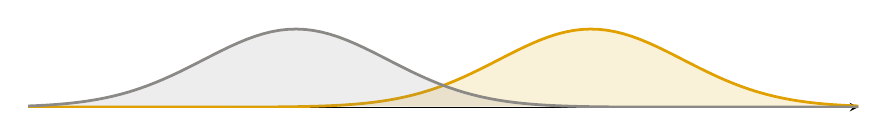
\begin{tikzpicture}
\begin{axis}[width=\linewidth, height=2.7cm, xmin=-4.5, xmax=4.5, ymin=0, ymax=0.45, axis x line=bottom, axis y line=none, ytick=\empty, xtick=\empty]
\addplot[domain=-4.5:4.5, samples=100, eHap, fill=eHap, fill opacity=0.15, line width=1pt] {exp(-(x-1.6)^2/2)/sqrt(2*pi)};
\addplot[domain=-4.5:4.5, samples=100, eNeu, fill=eNeu, fill opacity=0.15, line width=1pt] {exp(-(x+1.6)^2/2)/sqrt(2*pi)};
\end{axis}
\end{tikzpicture}\\
{\scriptsize $D = \sqrt{(\mu_k-\mu_l)^{\top}\Sigma^{-1}(\mu_k-\mu_l)}$}
\end{column}
\begin{column}{0.30\textwidth}
\centering
{\scriptsize\T{分類器の向き $v$ に射影}{\EN}}\\
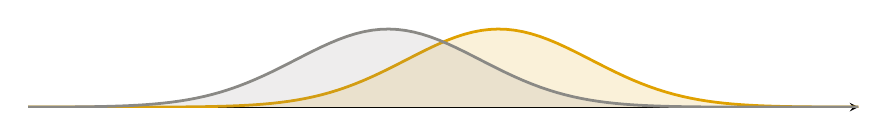
\begin{tikzpicture}
\begin{axis}[width=\linewidth, height=2.7cm, xmin=-4.5, xmax=4.5, ymin=0, ymax=0.45, axis x line=bottom, axis y line=none, ytick=\empty, xtick=\empty]
\addplot[domain=-4.5:4.5, samples=100, eHap, fill=eHap, fill opacity=0.15, line width=1pt] {exp(-(x-0.6)^2/2)/sqrt(2*pi)};
\addplot[domain=-4.5:4.5, samples=100, eNeu, fill=eNeu, fill opacity=0.15, line width=1pt] {exp(-(x+0.6)^2/2)/sqrt(2*pi)};
\end{axis}
\end{tikzpicture}\\
{\scriptsize $d = \dfrac{v^{\top}(\mu_k-\mu_l)}{\sqrt{v^{\top}\Sigma v}} \;\le\; D$}
\end{column}
\end{columns}
\vspace{0.2em}
\[
\textcolor{cDisc}{\textbf{\T{向きの損}{\EN}}}\quad A(D, 0) - A(d, 0)
\]
\msg{\T{向きのずれは，切片をどう当て直しても取り戻せない．$W$ を変える情報が要る}{\EN}}
\fnote{\T{$\mu_k$，$\Sigma$：感情 $k$ の特徴の平均と，感情に共通の共分散．模式図の値は $D \approx 3.2$，$d \approx 1.2$（左の楕円から計算）．実際の $D$ は縮小 LDA で推定する}{\EN}}
\end{frame}

% ---------------------------------------------------------------------
\begin{frame}{\T{損を 2 つに分け，情報源ごとにどちらを減らしたかを数える}{\EN}}
\centering
\[
\underbrace{A(D, 0) - A(d, o)}_{\text{\T{対の損（最良の線形判別との差）}{\EN}}}
\;=\;
\underbrace{\big[A(D, 0) - A(d, 0)\big]}_{\textcolor{cDisc}{\text{\T{向きの損}{\EN}}}}
\;+\;
\underbrace{\big[A(d, 0) - A(d, o)\big]}_{\textcolor{cCrit}{\text{\T{切片の損}{\EN}}}}
\]
\vspace{0.1em}
\scriptsize
\renewcommand{\arraystretch}{1.15}
\begin{tabular}{@{}p{0.2\linewidth}p{0.37\linewidth}p{0.37\linewidth}@{}}
\toprule
\T{設定}{\EN} & \textcolor{cDisc}{\T{向きの損の測り方}{\EN}} & \textcolor{cCrit}{\T{切片の分の測り方}{\EN}} \\
\midrule
\T{単一ソース設定，全ソース設定}{\EN} & \T{上の式の対の模型．6 対の平均}{\EN} & \T{「切片だけを K 本で直す方法」の UAR の上がり幅（模型の値は誤差と同じ大きさなので使わない）}{\EN} \\
\T{LOCO 設定}{\EN} & \T{候補の全ラベルで学んだ $W^{*}$ との UAR の差のうち，切片を当て直しても残る分}{\EN} & \T{同じ差のうち，切片の当て直しで減る分}{\EN} \\
\bottomrule
\end{tabular}
\msg{\T{同じ誤りの分け方で，4 つの情報源がそれぞれどちらの損を減らすかを数える}{\EN}}
\fnote{\T{対の模型の向きの損は顔を除いて当てはまりの基準を満たした．LOCO 設定で確かめに不合格の 5 組は「向き」と呼ばない（補足 2）}{\EN}}
\end{frame}

%% D．結果の前半：ターゲットのラベルとソースのコーパス（単一ソース設定．スライド 19〜25）
%% 数の出どころ：results/e76_analysis/（E76 の再解析．コミット e39e54a．話者を単位にした区間）．scripts/export_figdata.py が書き出す．
%% 同じ 7 群・反復 0〜9 での再推定で，確認ではない（docs/exploratory-analyses.md の E76 11 節）．英語は後で訳す（\EN）
\setband{\T{結果の前半：ターゲットのラベルとソースのコーパス}{\EN}}
\pgfplotsset{
  kindx/.style={xtick={1,...,8}, xticklabels={A, A(Hu), V, T, AV, VT, AT, AVT}, xticklabel style={font=\scriptsize}, xmin=0.4, xmax=8.6},
}

% ---------------------------------------------------------------------
\begin{frame}{\T{単一ソース設定：1 つのソースの全発話とターゲットの K 本を合併して学ぶ}{\EN}}
\begin{columns}[T]
\begin{column}{0.46\textwidth}
\centering
\begin{adjustbox}{max width=\linewidth}
\begin{tikzpicture}[x=1cm, y=1cm]
  \node[srcbox, minimum width=2.4cm, minimum height=1.0cm] (s) at (0,1.2) {\T{ソース 1 つの全発話}{\EN}};
  \node[tgtbox, minimum width=2.4cm] (k) at (0,0) {\T{ターゲットの K 本}{\EN}};
  \node[big, fill=cLearn!10, draw=cLearn, minimum width=2.2cm] (m) at (3.4,0.6) {\T{合併}{\EN}\\[-2pt]{\tiny\T{1 つの分類器}{\EN}}};
  \node[tgtbox, minimum width=2.4cm] (k2) at (0,-1.3) {\T{ターゲットの K 本}{\EN}};
  \node[big, fill=white, minimum width=2.2cm] (t) at (3.4,-1.3) {\T{ターゲットのみ}{\EN}};
  \draw[arr] (s.east) -- (m); \draw[arr] (k.east) -- (m); \draw[arr] (k2) -- (t);
  \node[font=\small, align=center] at (6.45,-0.35) {gain\\$=$ \T{合併}{\EN}\\$-$ \T{ターゲットのみ}{\EN}};
  \draw[mMuted, decorate, decoration={brace, amplitude=5pt}] (4.7,1.1) -- (4.7,-1.8);
\end{tikzpicture}
\end{adjustbox}
\end{column}
\begin{column}{0.52\textwidth}
\footnotesize
\T{%
\begin{itemize}
\item 7 群がそれぞれターゲット．ソースは 1 つずつ（IEMOCAP 即興と台本の組は除く）
\item 特徴は 8 種類：A（WavLM），A(Hu)（HuBERT），V，T，AV，VT，AT，AVT（つないだ融合）
\item 組の数：A・A(Hu) 40，V・AV 28，言葉を含む 4 種類 10
\item K ∈ \{1, 5, 10, 25, 50, 全件\}．K 本の抜き方とテストの分割を変えた反復 10 回
\item 区間：話者を単位にした 2 段の引き直し（95\%）．組ごとの判定は Holm で補正
\end{itemize}}{\EN}
\end{column}
\end{columns}
\fnote{\T{合併の分類器の罰則の強さは，ソースのみの分類器で選んだ値に固定した．この節の値は，主張を作ったのと同じ 7 群・反復での再推定で，確認ではない（E76）}{\EN}}
\end{frame}

% ---------------------------------------------------------------------
\begin{frame}{\T{ターゲットのラベルが少ないうちは，ソースを混ぜると上がる}{\EN}}
\begin{columns}[T]
\begin{column}{0.55\textwidth}
\centering
\begin{tikzpicture}
\begin{axis}[width=\linewidth, height=5.0cm, xtick={1,...,6}, xticklabels={1,5,10,25,50,\T{全件}{\EN}}, xlabel={K}, ylabel={\T{gain（合併 − ターゲットのみ）}{\EN}},
  ymin=-7, ymax=15, xmin=0.7, xmax=6.3, ymajorgrids, legend style={at={(0.98,0.98)}, anchor=north east, font=\tiny, legend columns=2}, legend cell align=left]
\addplot[kA, line width=1.2pt, mark=*, mark size=1.2pt] table[x=x, y=a, col sep=comma, comment chars={\#}]{figures/gain_curve.csv};
\addplot[kAH, line width=1.0pt, mark=*, mark size=1.2pt] table[x=x, y=ah, col sep=comma, comment chars={\#}]{figures/gain_curve.csv};
\addplot[kV, line width=1.2pt, mark=*, mark size=1.2pt] table[x=x, y=v, col sep=comma, comment chars={\#}]{figures/gain_curve.csv};
\addplot[kT, line width=1.2pt, mark=*, mark size=1.2pt] table[x=x, y=t, col sep=comma, comment chars={\#}]{figures/gain_curve.csv};
\addplot[kAV, line width=1.0pt, mark=*, mark size=1.2pt] table[x=x, y=av, col sep=comma, comment chars={\#}]{figures/gain_curve.csv};
\addplot[kVT, line width=1.0pt, mark=*, mark size=1.2pt] table[x=x, y=vt, col sep=comma, comment chars={\#}]{figures/gain_curve.csv};
\addplot[kAT, line width=1.0pt, mark=*, mark size=1.2pt] table[x=x, y=at, col sep=comma, comment chars={\#}]{figures/gain_curve.csv};
\addplot[kAVT, line width=1.0pt, mark=*, mark size=1.2pt] table[x=x, y=avt, col sep=comma, comment chars={\#}]{figures/gain_curve.csv};
\addplot[mMuted, dashed, domain=0.7:6.3] {0};
\legend{A, A(Hu), V, T, AV, VT, AT, AVT}
\end{axis}
\end{tikzpicture}
\end{column}
\begin{column}{0.43\textwidth}
\centering
{\scriptsize\T{K = 1 の gain と 95\% 区間}{\EN}}\\
\begin{tikzpicture}
\begin{axis}[width=\linewidth, height=4.6cm, kindx, ymin=0, ymax=16, ymajorgrids]
\addplot[only marks, mark=*, mark size=2pt, mAccentBlue, error bars/.cd, y dir=both, y explicit, error bar style={line width=1pt}]
  table[x=x, y=g, y error plus=ep, y error minus=em, col sep=comma, comment chars={\#}]{figures/gain_k1.csv};
\end{axis}
\end{tikzpicture}
\end{column}
\end{columns}
\msg{\T{K = 1 では 8 種類すべてで区間が 0 より上（\N{gonemink} \N{gonemin}〜\N{gonemaxk} \N{gonemax} ポイント）}{\EN}}
\fnote{\T{gain は種類の組の平均．組ごとに Holm で補正して「上」と言える組（K = 1）：T・AT・VT・AVT 10/10，AV \N{goneupav}/\N{gonenav}，A \N{goneupa}/\N{gonena}，A(Hu) \N{goneupah}/\N{gonenah}，V \N{goneupv}/\N{gonenv}．出どころ：e76a\_1\_kind.csv}{\EN}}
\end{frame}

% ---------------------------------------------------------------------
\begin{frame}{\T{ターゲットのラベルが全件あると，ソースを混ぜると下がる}{\EN}}
\centering
\begin{tikzpicture}
\begin{axis}[width=0.7\linewidth, height=4.6cm, kindx, ymin=-7, ymax=1, ymajorgrids, ylabel={\T{gain（K = 全件）}{\EN}}]
\addplot[only marks, mark=*, mark size=2.2pt, mBad, error bars/.cd, y dir=both, y explicit, error bar style={line width=1pt}]
  table[x=x, y=g, y error plus=ep, y error minus=em, col sep=comma, comment chars={\#}]{figures/gain_all.csv};
\addplot[mMuted, dashed, domain=0.4:8.6] {0};
\end{axis}
\end{tikzpicture}
\msg{\T{平均は 8 種類すべてで区間が 0 より下（A \N{galla}，区間 \N{gallcia}〜\N{gallcihia}）}{\EN}}
\fnote{\T{ただし組ごとに Holm で補正して「下」と言える組は半分未満：A \N{galldowna}/\N{gonena}，A(Hu) \N{galldownah}/\N{gonenah}，V \N{galldownv}/\N{gonenv}，AV \N{galldownav}/\N{gonenav}，T \N{galldownt}/10，AT \N{galldownat}/10，VT \N{galldownvt}/10，AVT \N{galldownavt}/10．「大きい K では下がる組がある」と書く}{\EN}}
\end{frame}

% ---------------------------------------------------------------------
\begin{frame}{\T{K 本が合併でしている仕事の大部分は，切片の直し（単独の声と顔）}{\EN}}
\centering
\begin{tikzpicture}
\begin{axis}[width=0.86\linewidth, height=4.5cm, kindx, ybar, bar width=7pt, ymin=-0.5, ymax=6.8, ymajorgrids, ylabel={\T{gain（ソースのみとの差，K = 5）}{\EN}},
  legend style={at={(0.5,1.02)}, anchor=south, font=\scriptsize, legend columns=2, /tikz/every even column/.append style={column sep=1em}}, legend cell align=left]
\addplot[mark=none, fill=cOther, draw=cOther, error bars/.cd, y dir=both, y explicit, error bar style={black, line width=0.6pt}] table[x=x, y=merge, y error plus=merge_ep, y error minus=merge_em, col sep=comma, comment chars={\#}]{figures/crit_merge_k5.csv};
\addplot[mark=none, fill=cCrit, draw=cCrit, error bars/.cd, y dir=both, y explicit, error bar style={black, line width=0.6pt}] table[x=x, y=crit, y error plus=crit_ep, y error minus=crit_em, col sep=comma, comment chars={\#}]{figures/crit_merge_k5.csv};
\legend{\T{合併（ソース＋K 本で学び直す）}{\EN}, \T{K 本で切片だけを直す}{\EN}}
\node[font=\scriptsize\bfseries, cCrit] at (axis cs:1,6.35) {\N{ratioa}};
\node[font=\scriptsize\bfseries, cCrit] at (axis cs:2,6.35) {\N{ratioah}};
\node[font=\scriptsize\bfseries, cCrit] at (axis cs:3,6.35) {\N{ratiov}};
\node[font=\scriptsize, mMuted] at (axis cs:5,6.35) {\N{ratioav}};
\end{axis}
\end{tikzpicture}
\msg{\T{切片だけの方法が，合併の gain の \N{ratioa}（A）・\N{ratiov}（V）倍を出す（K = 5）}{\EN}}
\fnote{\T{gain はソースのみの分類器からの UAR の差．上の数は「切片だけ ÷ 合併」（A(Hu) \N{ratioah}，AV \N{ratioav}）．言葉を含む種類は gain そのものが小さい．この結論は合併の学習器に限る．切片の罰則を 10 倍にすると，A の切片だけの方法の gain は \N{crita} → \N{critlta} に下がる．出どころ：e76a\_4\_kind.csv（G\_merge，G\_crit）}{\EN}}
\end{frame}

% ---------------------------------------------------------------------
\begin{frame}{\T{切片は，ラベル無しで特徴の平均を引くだけで直せる}{\EN}}
\centering
\begin{tikzpicture}
\begin{axis}[width=0.86\linewidth, height=4.5cm, kindx, ybar, bar width=6pt, ymin=-1.2, ymax=6.2, ymajorgrids, ylabel={\T{gain（ソースのみとの差，K = 5）}{\EN}},
  legend style={at={(0.5,1.02)}, anchor=south, font=\scriptsize, legend columns=3, /tikz/every even column/.append style={column sep=0.8em}}, legend cell align=left]
\addplot[mark=none, fill=kT, draw=kT, error bars/.cd, y dir=both, y explicit, error bar style={black, line width=0.6pt}] table[x=x, y=center, y error plus=center_ep, y error minus=center_em, col sep=comma, comment chars={\#}]{figures/crit_merge_k5.csv};
\addplot[mark=none, fill=cCrit, draw=cCrit, error bars/.cd, y dir=both, y explicit, error bar style={black, line width=0.6pt}] table[x=x, y=crit, y error plus=crit_ep, y error minus=crit_em, col sep=comma, comment chars={\#}]{figures/crit_merge_k5.csv};
\addplot[mark=none, fill=cCrit!35, draw=cCrit, error bars/.cd, y dir=both, y explicit, error bar style={black, line width=0.6pt}] table[x=x, y=critc, y error plus=critc_ep, y error minus=critc_em, col sep=comma, comment chars={\#}]{figures/crit_merge_k5.csv};
\legend{\T{平均を引く（ラベル無し）}{\EN}, \T{K 本で切片を直す}{\EN}, \T{平均を引いた後に K 本で切片を直す}{\EN}}
\end{axis}
\end{tikzpicture}
\msg{\T{平均を引く gain は切片直しとほぼ同じ（A \N{centera} 対 \N{crita}）．その後の切片直しは残らない}{\EN}}
\fnote{\T{どれもソースのみの分類器からの gain．平均を引いた後の切片直しは，8 種類とも区間の下端が 0 を超えない（AV は 0 より下）．平均はテストの発話も含めて取る．候補だけの平均では，平均を引く gain は A \N{centerpoola}，その後の切片直しは A だけ \N{critcpoola}（区間 \N{critcpoolloa}〜\N{critcpoolhia}）で 0 より上．出どころ：e76a\_4\_kind.csv}{\EN}}
\end{frame}

% ---------------------------------------------------------------------
\begin{frame}{\T{声と言葉では，向きのずれはラベルを足しても少しずつしか直らない}{\EN}}
\hosoku{supp:qderiv}{\T{式の導出}{\EN}}
\centering
\begin{adjustbox}{max width=\linewidth, max totalheight=0.53\textheight}
\begin{tikzpicture}[x=1cm, y=1cm]
  % 左：K 本の平均の差の向き（白色化した座標の模式）
  \node[font=\small\bfseries, anchor=west] at (-0.2,3.35) {\T{なぜ遅いか（模式図）}{\EN}};
  \coordinate (O) at (0,0.6);
  \draw[cDisc, -{Stealth[length=2.6mm]}, line width=1.6pt] (O) -- (4.2,0.6);
  \node[font=\scriptsize, text=cDisc] at (2.1,0.3) {\T{最良の向き（長さ $D$）}{\EN}};
  \draw[mBad, -{Stealth[length=2.2mm]}, line width=1.1pt] (4.2,0.6) -- (4.2,3.0);
  \node[font=\scriptsize, text=mBad, anchor=west, align=left] at (4.3,2.75) {\T{雑音}{\EN}\\\T{（K = 1）}{\EN}};
  \draw[mBad!40, -{Stealth[length=2.2mm]}, line width=2.2pt] (4.2,0.6) -- (4.2,1.36);
  \node[font=\scriptsize, text=mBad!70, anchor=west, align=left] at (4.3,1.15) {\T{雑音}{\EN}\\\T{（K = 10）}{\EN}};
  \draw[mBad, dashed, line width=0.9pt] (O) -- (4.2,3.0);
  \draw[mBad!50, dashed, line width=0.9pt] (O) -- (4.2,1.36);
  \draw[mMuted] (1.2,0.6) arc[start angle=0, end angle=29.7, radius=1.2];
  \node[font=\scriptsize] at (1.45,0.92) {$\theta$};
  \node[font=\scriptsize, align=left, anchor=north west, text width=5.8cm] at (-0.2,-0.05) {\T{K 本の平均の差の向き（破線）は，最良の向きに雑音が乗ったもの．雑音は多くの次元に散らばり，大きさは $1/\sqrt{K}$ でしか縮まない}{\EN}};
  \node[font=\small, anchor=north west] at (-0.2,-1.35) {$\dfrac{d_T(K)}{D} = \cos\theta = \dfrac{1}{\sqrt{1 + q/K}}$};
  % 右：K を増やしたときの離れ方の比
  \begin{axis}[at={(6.9cm,-2.5cm)}, anchor=south west, width=8.4cm, height=5.6cm, xmode=log, xmin=1, xmax=50, xtick={1,5,10,25,50}, xticklabels={1,5,10,25,50},
    xlabel={\T{ターゲットのラベル K（感情ごとの本数）}{\EN}}, ylabel={\T{離れ方の比 $d_T(K)/D$}{\EN}}, ymin=0, ymax=1.1, ytick={0,0.25,0.5,0.75,1}, ymajorgrids, clip=false,
    legend style={at={(0.5,1.03)}, anchor=south, font=\scriptsize, legend columns=2, /tikz/every even column/.append style={column sep=0.8em}}, legend cell align=left]
  \addplot[kV, line width=1.3pt, restrict expr to domain={\thisrow{inrange}}{1:1}] table[x=K, y=v, col sep=comma, comment chars={\#}]{figures/q_curve.csv};
  \addplot[kA, line width=1.3pt, restrict expr to domain={\thisrow{inrange}}{1:1}] table[x=K, y=a, col sep=comma, comment chars={\#}]{figures/q_curve.csv};
  \addplot[kT, line width=1.3pt, restrict expr to domain={\thisrow{inrange}}{1:1}] table[x=K, y=t, col sep=comma, comment chars={\#}]{figures/q_curve.csv};
  \addplot[mMuted, dashed, line width=0.9pt, domain=1:50, samples=2] {1};
  \legend{\T{顔}{\EN}（$q$ = \N{qv}）, \T{声}{\EN}（$q$ = \N{qa}）, \T{言葉}{\EN}（$q$ = \N{qt}）, \T{$d_T = D$（物差し）}{\EN}}
  \addplot[kV, line width=1pt, dashed, forget plot, restrict expr to domain={\thisrow{inrange}}{0:0}] table[x=K, y=v, col sep=comma, comment chars={\#}]{figures/q_curve.csv};
  \addplot[kA, line width=1pt, dashed, forget plot, restrict expr to domain={\thisrow{inrange}}{0:0}] table[x=K, y=a, col sep=comma, comment chars={\#}]{figures/q_curve.csv};
  \addplot[kT, line width=1pt, dashed, forget plot, restrict expr to domain={\thisrow{inrange}}{0:0}] table[x=K, y=t, col sep=comma, comment chars={\#}]{figures/q_curve.csv};
  \addplot[kV, only marks, mark=square*, mark size=2pt, forget plot] table[x=K, y=v, col sep=comma, comment chars={\#}]{figures/q_pts.csv};
  \addplot[kA, only marks, mark=*, mark size=2pt, forget plot] table[x=K, y=a, col sep=comma, comment chars={\#}]{figures/q_pts.csv};
  \addplot[kT, only marks, mark=triangle*, mark size=2.4pt, forget plot] table[x=K, y=t, col sep=comma, comment chars={\#}]{figures/q_pts.csv};
  \draw[mMuted, densely dotted] (axis cs:10,0) -- (axis cs:10,1.1);
  \end{axis}
\end{tikzpicture}
\end{adjustbox}
\msg{\T{古典の式と同じ形の，母数 1 つの経験式で K ≤ 10 の直り方を要約した．K = 10 でも離れ方は $D$ の \N{dtraten} 倍（声），\N{dtrtten} 倍（言葉）}{\EN}}
\fnote{\T{$d_T(K)$：K 本だけの分類器の向きで測った離れ方．$D$：半分の話者で学んだ縮小 LDA の向きでの離れ方で，比べるための物差し（全件の到達点より小さい．次の 5 ページで補う）．点は実測，実線は K = 1, 5, 10 に当てた式，破線は延長．声と顔では K を 1 つ抜いた予測で 2 母数の形の方が良いターゲットが多い（$D$ で声 \N{qlooa}/\N{qna}，顔 \N{qloov}/\N{qnv}．$D'$ で \N{qloodpa}/\N{qndpa}，\N{qloodpv}/\N{qndpv}）ので，1 母数の形は K ≤ 50 の曲線を表さないとみなし，$q$ は K ≤ 10 の要約に使う．左は模式図．出どころ：e76a\_3\_dT.csv，e76a\_3\_q\_targets.csv}{\EN}}
\end{frame}

% ---------------------------------------------------------------------
% 2026-11-11 追加：33 ページへの質問（研究者「これは理論？導出も見せて．何が言えるんですか？今回の結果は理論に則った？A，V，T の違いは？」）への答え 5 枚
\begin{frame}{\T{前のページの式は定理ではなく，古典の式と同じ形の経験式である}{\EN}}
\footnotesize
\T{%
\begin{itemize}
\item \textbf{何を表す式か}：K 本だけで学んだ分類器の向きで測った 2 つの感情の離れ方 $d_T(K)$ が，K を増やすと $D$ に近づく速さを，母数 $q$ 1 つで表す
\item \textbf{どこから来たか}：2 つの感情の山を正規分布とみなし，「K 本の平均の差の向き」と「最良の向き」の角度を計算した簡単なモデルから出した（導出は次のページ）．同じ形の項（向きの誤差が $\propto 1/K$）は，線形判別の誤判別率を標本の数で展開した古典の結果（Okamoto 1963，Raudys 1998）に現れる
\item \textbf{証明した定理ではない}：導出は 4 つの仮定を置いた近似である．今回のデータでは，仮定 (d)（$D$ が到達点）は満たさないことが分かった（3 ページ後）．古典の展開は標本の数が特徴の次元より十分多いときの式で，今回は次元 512〜1,024 に対し K ≤ 50 である
\item \textbf{記録の決まり}：この式は「K ≫ p の古典の展開と同じ形の経験式」と書き，$q$ を「有効次元」とは呼ばない（E76 の設計で計算の前に決めた）
\end{itemize}}{\EN}
\msg{\T{確かめたのは式の形の当てはまりで，式が成り立つ理由ではない}{\EN}}
\fnote{\T{Okamoto 1963 は再掲（Shutoh の技術報告）で読み，原著は確かめていない．古典の係数から向きの項が出ることは本研究の計算で，「閾値と向きに分ける」解釈は原著に無い（docs/related-work.md 1.13・1.14 節）}{\EN}}
\end{frame}

% ---------------------------------------------------------------------
\begin{frame}{\T{導出：K 本の平均の差の向きは，最良の向きに雑音が乗ったもの}{\EN}}
\begin{columns}[T]
\begin{column}{0.56\textwidth}
\footnotesize
\T{%
\begin{enumerate}
\item 特徴を感情に共通の共分散で白色化する．2 つの感情の平均の差は $D\,w$（$w$：最良の向きの単位ベクトル）
\item 感情ごとに K 本で平均を取ると，差の推定は $\hat m = D\,w + \varepsilon$．$\varepsilon$ の各成分の分散は $2/K$
\item K 本だけの分類器の向き $u$ を $\hat m$ の向きとみなす（仮定）
\item $u$ で測った離れ方は $d_T = u^{\top}(D\,w) = D\cos\theta$
\item $w$ の向きの雑音を無視し，雑音が効く次元を $p$ 個とすると $\cos^2\theta \approx \dfrac{D^2}{D^2 + 2p/K}$
\item よって $d_T(K) = \dfrac{D}{\sqrt{1 + q/K}}$，$q = \dfrac{2p}{D^2}$
\end{enumerate}}{\EN}
\end{column}
\begin{column}{0.42\textwidth}
\footnotesize
\textbf{\T{置いた仮定}{\EN}}\par
\T{(a) 2 つの山は共分散が同じ正規分布．(b) 雑音は等方．(c) 分類器の向き ＝ 平均の差の向き．(d) $D$ は K → ∞ の到達点}{\EN}\par\vspace{0.6em}
\textbf{\T{数値例（声の $q$ ＝ \N{qa}）}{\EN}}\par
\renewcommand{\arraystretch}{1.15}
\begin{tabular}{@{}lcccc@{}}
\toprule
K & 1 & 5 & 10 & 50 \\
$d_T/D$（\T{式}{\EN}） & \N{qfaone} & \N{qfafive} & 0.\N{qtena} & \N{qfafifty} \\
\bottomrule
\end{tabular}\par\vspace{0.4em}
\T{$p$ は測っていない．$q$ は K = 1, 5, 10 の実測に当てはめて決めた}{\EN}
\end{column}
\end{columns}
\msg{\T{雑音は $1/\sqrt{K}$ でしか縮まないので，向きは少しずつしか最良に近づかない}{\EN}}
\fnote{\T{表の値は式の値で，実測ではない（実測は次のページ）．記録：docs/exploratory-analyses.md の E28 の 9 節（3128 行〜）．補足 12 に同じ導出}{\EN}}
\end{frame}

% ---------------------------------------------------------------------
\begin{frame}{\T{言えること：K = 10 でも，離れ方は $D$ の声 \N{dtraten} 倍，言葉 \N{dtrtten} 倍にとどまる}{\EN}}
\centering
\small
\renewcommand{\arraystretch}{1.25}
\begin{tabular}{@{}lcccccc@{}}
\toprule
\T{実測の $d_T(K)/D$}{\EN} & K = 1 & 5 & 10 & 25 & 50 & \T{全件}{\EN} \\
\midrule
\textcolor{kA}{\T{声}{\EN}} & \N{dtraone} & \N{dtrafive} & \N{dtraten} & \N{dtratf} & \N{dtrafifty} & \N{dtraall} \\
\textcolor{kV}{\T{顔}{\EN}} & \N{dtrvone} & \N{dtrvfive} & \N{dtrvten} & \N{dtrvtf} & \N{dtrvfifty} & \N{dtrvall} \\
\textcolor{kT}{\T{言葉}{\EN}} & \N{dtrtone} & \N{dtrtfive} & \N{dtrtten} & \N{dtrttf} & \N{dtrtfifty} & \N{dtrtall} \\
\bottomrule
\end{tabular}
\par\vspace{0.5em}
\footnotesize
\T{%
\begin{itemize}
\item 言えること：声と言葉では，K 本だけで学ぶ分類器の向きは K = 10 でも全件の到達点より大きく劣る．向きを直すには，K 本以外の情報が要る（この資料の後半の問いの出発点）
\item 言えないこと：1 を超える値は，$D$ が全件の到達点より小さいことを示す．$D$ を基準にした割合は「最良の向きの何割か」ではなく「半分の話者で学んだ LDA の向きの何割か」である
\end{itemize}}{\EN}
\msg{\T{全件で 1 を超えるので，$D$ は最良の向きではなく比べる物差しとして読む}{\EN}}
\fnote{\T{全件の到達点 $D'$ を基準にすると，K = 10 で声 \N{dtrpaten}，顔 \N{dtrpvten}，言葉 \N{dtrptten} 倍．単一ソース設定のターゲットのみの分類器．6 対で平均し，ターゲット（声 \N{qna}，顔 \N{qnv}，言葉 \N{qnt}）の中央値を取った．出どころ：results/e76\_analysis/e76a\_3\_dT.csv（rule=main）}{\EN}}
\end{frame}

% ---------------------------------------------------------------------
\begin{frame}{\T{式の仮定どおりか：声・顔は 2 母数の形が良く，仮定も満たさない}{\EN}}
\centering
\scriptsize
\renewcommand{\arraystretch}{1.3}
\begin{tabular}{@{}p{0.36\linewidth}ccc p{0.2\linewidth}@{}}
\toprule
\T{確かめ（計算の前に基準を決めた）}{\EN} & \textcolor{kA}{\T{声}{\EN}} & \textcolor{kV}{\T{顔}{\EN}} & \textcolor{kT}{\T{言葉}{\EN}} & \T{判定}{\EN} \\
\midrule
\T{形：K = 1〜50 の残差が基準の中（ターゲットの数）}{\EN} & \multicolumn{3}{c}{\T{\N{qfitn} ターゲットすべて}{\EN}} & \textcolor{mGood}{\T{合う}{\EN}} \\
\T{K を 1 つ抜いて予測したとき，2 母数の形の方が良いターゲット（$D$／$D'$）}{\EN} & \N{qlooa}/\N{qna}，\N{qloodpa}/\N{qndpa} & \N{qloov}/\N{qnv}，\N{qloodpv}/\N{qndpv} & \N{qloot}/\N{qnt}，\N{qloodpt}/\N{qndpt} & \textcolor{mBad}{\T{声・顔は 1 母数では足りない}{\EN}} \\
\T{仮定 (d)：$D$ が到達点．全件で $d_T > D$ になった（ターゲット，対）}{\EN} & \N{gtdaall}/\N{gtdna} & \N{gtdvall}/\N{gtdnv} & \N{gtdtall}/\N{gtdnt} & \textcolor{mBad}{\T{満たさない}{\EN}} \\
\T{6 対で $q$ が共通（$q$ の最大 ÷ 最小．基準 3 以下）}{\EN} & \N{qpairratioa} & \N{qpairratiov} & \N{qpairratiot} & \textcolor{mBad}{\T{満たさない}{\EN}} \\
\bottomrule
\end{tabular}
\msg{\T{式は K ≤ 10 の要約として使えるが，仮定した仕組みで起きたとは言えない}{\EN}}
\fnote{\T{2 母数の形：$D$ も当てる形と $d = aK^b$．言葉は設計の条件（$D$ と $D'$ の両方で 3 分の 2 以上）に当たらないので $q$ を出す．$q$ は 6 対の平均の曲線の係数として読む．仮定 (a)〜(c) は直接は測っていない．$D$ の代わりに全件の到達点 $D'$ を基準にすると $q$ は声 \N{qdpa}，顔 \N{qdpv}，言葉 \N{qdpt}（次のページ）．記録：docs/exploratory-analyses.md の E76 の 11 節（9009〜9010 行）．出どころ：e76a\_3\_q\_targets.csv，e76a\_3\_dT\_gt\_D.csv}{\EN}}
\end{frame}

% ---------------------------------------------------------------------
\begin{frame}{\T{A・V・T の違い：中央値の $q$ は顔 < 声 < 言葉．顔の値は基準 $D$ に強く依る}{\EN}}
\begin{columns}[T]
\begin{column}{0.5\textwidth}
\centering
\scriptsize
\renewcommand{\arraystretch}{1.25}
\begin{tabular}{@{}lccc@{}}
\toprule
 & \textcolor{kA}{\T{声}{\EN}} & \textcolor{kV}{\T{顔}{\EN}} & \textcolor{kT}{\T{言葉}{\EN}} \\
\midrule
\T{$q$（$D$ で当てる）}{\EN} & \N{qa} & \N{qv} & \N{qt} \\
\T{$q$（$D'$ で当てる）}{\EN} & \N{qdpa} & \N{qdpv} & \N{qdpt} \\
\T{ターゲットごとの $q$}{\EN} & \N{qmina}〜\N{qmaxa} & \N{qminv}〜\N{qmaxv} & \N{qmint}〜\N{qmaxt} \\
\T{$D$ の中央値}{\EN} & \N{dmeda} & \N{dmedv} & \N{dmedt} \\
\T{$D'/D$ の中央値}{\EN} & \N{dpda} & \N{dpdv} & \N{dpdt} \\
\T{K = 10 で $d_T > D$ の対}{\EN} & \N{gtdaten}/\N{gtdna} & \N{gtdvten}/\N{gtdnv} & \N{gtdtten}/\N{gtdnt} \\
\bottomrule
\end{tabular}
\end{column}
\begin{column}{0.48\textwidth}
\footnotesize
\T{%
\begin{itemize}
\item 顔は K = 10 ですでに半分近くの対で $d_T > D$．$D$ が小さすぎ，$D$ で当てた $q$ = \N{qv} は小さく出る．$D'$ どうしでは顔 \N{qdpv}，声 \N{qdpa}，言葉 \N{qdpt} で，差は小さくなる
\item 同じターゲットで比べると，言葉が声より遅いのは $D$ でも $D'$ でも \N{tcommond} 中 \N{tslowerd}（MELD は逆：$D$ で言葉 \N{qmeldtd}，声 \N{qmeldad}）
\item ターゲットごとの $q$（$D$ で当てた値）の最大 ÷ 最小は声 \N{qratioa}，顔 \N{qratiov}，言葉 \N{qratiot} 倍
\item 言葉の向きが遅い理由は測っていない
\end{itemize}}{\EN}
\end{column}
\end{columns}
\msg{\T{中央値の並びは $D$ でも $D'$ でも同じだが例外がある．顔の速さは $D$ に依る}{\EN}}
\fnote{\T{読み（未検証）：顔は表情のラベルで微調整したモデルの特徴で，感情の向きが最初から目立ちうる．$D'$：同じ学習器を全件で学んだときの離れ方．出どころ：e76a\_3\_q\_summary.csv，q\_targets.csv，dT.csv}{\EN}}
\end{frame}

% ---------------------------------------------------------------------
\begin{frame}{\T{ここまでの答えと，残る問い}{\EN}}
\centering
\small
\renewcommand{\arraystretch}{1.3}
\begin{tabular}{@{}lll@{}}
\toprule
\T{情報源}{\EN} & \textcolor{cCrit}{\T{切片のずれ}{\EN}} & \textcolor{cDisc}{\T{向きのずれ}{\EN}} \\
\midrule
\T{① ターゲットの K 本}{\EN} & \T{速く直す（合併の gain の大部分）}{\EN} & \T{遅くしか直さない（$q$）}{\EN} \\
\T{② ソースのコーパス（合併）}{\EN} & \T{K が小さいとき gain が正．全件では負}{\EN} & — \\
\T{③ ラベル無し（平均を引く）}{\EN} & \T{ラベル無しで直す}{\EN} & \textcolor{cAsk}{\textbf{?}} \\
\T{④ ほかのモダリティ}{\EN} & \textcolor{cAsk}{\textbf{?}} & \textcolor{cAsk}{\textbf{?}} \\
\bottomrule
\end{tabular}
\vspace{0.8em}
\band{cAsk}{\T{問い}{\EN}}{\T{ラベルを増やさずに，向きのずれを直せるものはあるか}{\EN}}
\end{frame}

%% E．結果の後半：ほかのモダリティの予測を使う提案（スライド 26〜34）
%% 数の出どころ：全ソース設定 results/e79/judge/units.csv（P5-*），results/e79_p4/judge/units.csv（P4）．
%% LOCO 設定 results/dai1/stats/families_flagged.csv（評価の回 ba98974）．scripts/export_figdata.py が書き出す．英語は後で訳す（\EN）
\setband{\T{学び直しの式}{\EN}}

% ---------------------------------------------------------------------
\begin{frame}{\T{学び直しの式：4 つの情報源は，式のどの項に入るか}{\EN}}
\centering
\resizebox{0.94\linewidth}{!}{$\displaystyle
\min_{W,\,b}\;
\underbrace{\frac{1}{|\mathcal{L}|}\sum_{(x,y)\in\mathcal{L}} \ell\big(Wx+b,\;y\big)}_{\textcolor{eAng}{\text{\T{① K 本の損失}{\EN}}}}
\;+\;
\underbrace{\lambda\,\|W-W_0\|^2+\lambda_b\,\|b-b_0\|^2}_{\textcolor{mAccentBlue}{\text{\T{② 出発点 $(W_0, b_0)$ への L2 正則化}{\EN}}}}
\;+\;
\underbrace{\frac{\mu}{|\mathcal{U}|}\sum_{x\in\mathcal{U}} \ell\big(Wx+b,\;q(x)\big)}_{\textcolor{kV}{\text{\T{④ 疑似ラベル $q$ の損失}{\EN}}}}
$}
\vspace{0.3em}
\begin{columns}[T]
\begin{column}{0.48\textwidth}
\footnotesize
\T{%
\begin{itemize}
\item \textcolor{eAng}{\textbf{①}}：ターゲットの K 本 × 4 感情（$\mathcal{L}$）の交差エントロピー
\item \textcolor{mAccentBlue}{\textbf{②}}：出発点はソースで学んだ分類器（K = 0 の分類器）．$\lambda$，$\lambda_b$ はメタ学習で選ぶ
\end{itemize}}{\EN}
\end{column}
\begin{column}{0.5\textwidth}
\footnotesize
\T{%
\begin{itemize}
\item \textcolor{kT}{\textbf{③}}：特徴 $x$ から，ターゲットのラベル無しの発話（$\mathcal{U}$）の平均を引く（LOCO 設定では標準偏差でも割る）
\item \textcolor{kV}{\textbf{④}}：$q(x)$ は LOCO 設定では声・顔・言葉の分類器の確率の積（全ソース設定では出所と重みの付け方を候補から選ぶ．p.~\pageref{prop:def}）．$\mu$ はメタ学習で選ぶ
\end{itemize}}{\EN}
\end{column}
\end{columns}
\msg{\T{後半では，$\mu = 0$（K 本だけ）と $\mu > 0$（提案）を比べる}{\EN}}
\fnote{\T{どの設定のどの学び方でどの項を使うかは，次のページの表}{\EN}}
\end{frame}

% ---------------------------------------------------------------------
\begin{frame}{\T{どの設定で，どの学び方に，どの項を使うか}{\EN}}
\centering
{\footnotesize \textcolor{eAng}{\T{① K 本の損失}{\EN}}\quad \textcolor{mAccentBlue}{\T{② ソース}{\EN}}\quad \textcolor{kT}{\T{③ ラベル無しの発話の平均を引く}{\EN}}\quad \textcolor{kV}{\T{④ 疑似ラベルの損失}{\EN}}\par}
\vspace{0.15em}
\scriptsize
\renewcommand{\arraystretch}{1.05}
\setlength{\tabcolsep}{4pt}
\begin{tabular}{@{}p{0.16\linewidth}p{0.19\linewidth}p{0.035\linewidth}p{0.22\linewidth}p{0.035\linewidth}p{0.22\linewidth}@{}}
\toprule
\T{学び方}{\EN} & \T{設定（使う部）}{\EN} & \textcolor{eAng}{①} & \textcolor{mAccentBlue}{②} & \textcolor{kT}{③} & \textcolor{kV}{④} \\
\midrule
\T{ターゲットのみ}{\EN} & \T{単一ソース（前半）}{\EN} & ○ & — & — & — \\
\T{ソースのみ}{\EN} & \T{単一ソース（前半）}{\EN} & — & \T{ソースの全発話で学ぶ}{\EN} & — & — \\
\T{合併}{\EN} & \T{単一ソース（前半）}{\EN} & ○ & \T{① にソースの全発話を足す}{\EN} & — & — \\
\T{平均を引く}{\EN} & \T{単一ソース（前半）}{\EN} & — & \T{ソースのみの分類器}{\EN} & ○ & — \\
\midrule
\T{K 本だけ（基準）}{\EN} & \T{全ソース，LOCO（後半）}{\EN} & ○ & \T{出発点への L2 正則化}{\EN} & ○ & —（$\mu = 0$） \\
\textbf{\T{提案}{\EN}} & \T{全ソース，LOCO（後半）}{\EN} & ○ & \T{出発点への L2 正則化}{\EN} & ○ & \T{ほかのモダリティを含む予測}{\EN} \\
\T{8 手法（比べる相手）}{\EN} & \T{全ソース（後半）}{\EN} & ○ & \T{出発点への L2 正則化}{\EN} & ○ & \T{手法ごとの項（同じモダリティ）}{\EN} \\
\bottomrule
\end{tabular}
\msg{\T{前半は学ぶデータの組み合わせを，後半は ④ の有無と中身を比べる}{\EN}}
\fnote{\T{出発点：全ソース設定ではターゲット以外の全コーパスで学んだ分類器，LOCO 設定ではソースのコーパスごとの分類器の平均．8 手法の T3A とラベル伝播は予測を作り直す操作}{\EN}}
\end{frame}

\setband{\T{結果の後半：ほかのモダリティの予測を使う提案}{\EN}}
\pgfplotsset{
  corpx/.style={xtick={1,2,3,4}, xticklabels={AFEW, IEMOCAP, MELD, MOSEI}, xticklabel style={font=\scriptsize}, xmin=0.5, xmax=4.5},
  jbar/.style={xbar stacked, bar width=13pt, xmin=0, xmax=100, axis x line*=bottom, axis y line*=left, y axis line style={draw=none}, ytick style={draw=none},
    xtick={0,25,50,75,100}, xticklabel style={font=\scriptsize},
    nodes near coords={\pgfmathprintnumber[fixed, precision=0]{\pgfplotspointmeta}}, every node near coord/.append style={font=\tiny},
    point meta=explicit},
}

% ---------------------------------------------------------------------
% 2026-11-11 追加：提案とは何かを 1 枚で（研究者「今何が提案手法かよくわからん」）
\begin{frame}{\T{提案：同じ発話の複数のモダリティの予測から疑似ラベルを作り，学び直す}{\EN}}
\label{prop:def}
\centering
\scriptsize
\renewcommand{\arraystretch}{1.2}
\begin{tabular}{@{}p{0.2\linewidth}p{0.75\linewidth}@{}}
\toprule
\T{使うもの}{\EN} & \T{ターゲットの K 本のラベル，ターゲットのラベル無しの発話（複数のモダリティがそろうもの），ソースで学んだ分類器（出発点）}{\EN} \\
\T{LOCO 設定の版（本番）}{\EN} & \T{疑似ラベルは声・顔・言葉の 3 つの分類器の確率の積で，感情ごとの総量をそろえる（次のページ）．K 本と疑似ラベルで声・顔・言葉・融合の分類器を学び直す．設定はメタ学習で選んで固定し，ほとんど既定値が選ばれた}{\EN} \\
\T{全ソース設定の版（探索）}{\EN} & \T{疑似ラベルの出所と重みの付け方を，条件ごとに仮のターゲットで候補から選ぶ．\N{oxn} の選択のうち，出所は各モダリティの分類器の積が \N{oxprod}，融合の分類器の予測が \N{oxpfk}，一致で重みをつけた版が \N{oxagree}．重みは総量をそろえる \N{oxbal}，確信度で切る \N{oxhard}，確率そのまま \N{oxraw}．AV の組では声と顔の 2 つの積}{\EN} \\
\T{比べる相手}{\EN} & \T{K 本だけ（疑似ラベルの項が無い版．学び直しの式の $\mu = 0$），同じモダリティのラベル無しの発話を使う 8 手法（全ソース設定），標準の適応の手法（LOCO 設定）}{\EN} \\
\T{提案ではないもの}{\EN} & \T{「なぜ上がるか」の下調べでは，疑似ラベルの出所を替えて比べる．中間層の下調べの疑似ラベルは顔と言葉の 2 つの積で，提案の疑似ラベルとは違う}{\EN} \\
\bottomrule
\end{tabular}
\msg{\T{疑似ラベルは，ほかのコーパスのデータを足すのではなく，同じ発話の複数のモダリティの予測（学び直す分類器自身のモダリティを含む）から作る}{\EN}}
\end{frame}

% ---------------------------------------------------------------------
\begin{frame}{\T{提案の作り方（LOCO 設定の版）：3 つの予測の積を疑似ラベルにする}{\EN}}
\hosoku{supp:pseudo}{\T{疑似ラベルの数値例}{\EN}}
\centering
\begin{adjustbox}{max width=\linewidth, max totalheight=0.64\textheight}
\begin{tikzpicture}[x=1cm, y=1cm]
  % ① 融合の分類器を K 本だけで学ぶ
  \node[font=\scriptsize\bfseries, align=center, text width=3.0cm, anchor=south] at (1.2,2.75) {\T{① 融合の分類器を K 本だけで学び，候補の発話に予測を付ける}{\EN}};
  \foreach \c [count=\r from 0] in {eNeu,eHap,eSad,eAng} {\foreach \i in {0,1,2} {\node[utt, fill=\c, draw=white, minimum size=2mm] at (0.55+0.27*\i,2.3-0.27*\r) {};}}
  \node[font=\tiny, anchor=west] at (1.3,1.9) {\T{K 本}{\EN}};
  \node[big, fill=white, draw=kAVT, line width=1pt, text width=2.2cm, minimum height=0.9cm] (f) at (1.2,0.75) {\T{融合の分類器}{\EN}};
  \draw[arr] (1.2,1.25) -- (f.north);
  % ② 声・顔・言葉の分類器を学び直す
  \node[font=\scriptsize\bfseries, align=center, text width=3.4cm, anchor=south] at (5.0,2.75) {\T{② 声・顔・言葉の分類器を，K 本 ＋ ① の予測で学び直す}{\EN}};
  \node[clf, draw=kA, line width=1pt, minimum width=2.4cm, font=\small] (ca) at (5.0,2.05) {\T{声の分類器}{\EN}};
  \node[clf, draw=kV, line width=1pt, minimum width=2.4cm, font=\small] (cv) at (5.0,1.25) {\T{顔の分類器}{\EN}};
  \node[clf, draw=kT, line width=1pt, minimum width=2.4cm, font=\small] (ct) at (5.0,0.45) {\T{言葉の分類器}{\EN}};
  \draw[arr] (f.east) -- (ca.west); \draw[arr] (f.east) -- (cv.west); \draw[arr] (f.east) -- (ct.west);
  % ③ 3 つの確率を掛ける
  \node[font=\scriptsize\bfseries, align=center, text width=2.6cm, anchor=south] at (8.3,2.75) {\T{③ 3 つの確率を掛け，感情ごとの総量をそろえる}{\EN}};
  \node[circle, draw=mDarkTeal, fill=cMod, line width=0.9pt, minimum size=0.8cm, font=\small\bfseries] (x) at (7.75,1.25) {$\times$};
  \draw[arr] (ca.east) -- (x); \draw[arr] (cv.east) -- (x); \draw[arr] (ct.east) -- (x);
  \node[draw=kAV, fill=cMod, rounded corners=3pt, minimum width=1.7cm, minimum height=1.7cm] (q) at (9.5,1.25) {};
  \node[font=\scriptsize\bfseries] at (9.5,1.85) {\T{疑似ラベル $q$}{\EN}};
  \foreach \c/\h [count=\i from 0] in {eNeu/0.25, eHap/0.85, eSad/0.12, eAng/0.18} {\fill[\c] (8.93+0.3*\i,0.55) rectangle ++(0.22,\h);}
  \draw[mMuted] (8.85,0.55) -- (10.15,0.55);
  \draw[arr] (x) -- (q);
  % ④ 4 つの分類器を学び直す
  \node[draw=cLearn, fill=cLearn!8, rounded corners=4pt, minimum width=12.6cm, minimum height=1.55cm] (band) at (5.6,-1.35) {};
  \node[font=\scriptsize\bfseries, anchor=north west, text width=12.2cm] at (-0.6,-0.6) {\T{④ 4 つの分類器を，出発点から K 本 ＋ $q$ で学び直す（出発点への L2 正則化つき）}{\EN}};
  \foreach \n/\col/\xx in {\T{声}{\EN}/kA/0.9, \T{顔}{\EN}/kV/3.6, \T{言葉}{\EN}/kT/6.3, \T{融合}{\EN}/kAVT/9.0} {\node[clf, draw=\col, line width=1pt, minimum width=2.2cm, font=\small] at (\xx,-1.7) {\n};}
  \draw[arr, line width=1.1pt] (q.south) -- (9.5,-0.55);
\end{tikzpicture}
\end{adjustbox}
\msg{\T{声の分類器は，顔と言葉の分類器の予測を含む $q$ から，ラベル無しの発話で学ぶ}{\EN}}
\fnote{\T{④の損失：K 本の交差エントロピー ＋ 候補の発話での $q$ との交差エントロピー ＋ 出発点への L2 正則化．$q$ の重み，K 本の倍率，L2 正則化の強さ，③の指数はメタ学習（次のページ）で選んで固定した．③の指数は（コーパス，K）\N{mlmainof} 個すべてで (1, 1, 1)（掛けるだけ）が選ばれた．模式図で，棒は実験の値ではない}{\EN}}
\end{frame}

% ---------------------------------------------------------------------
\begin{frame}{\T{メタ学習：2 つの設定で，ハイパーパラメータをソースだけで選んだ}{\EN}}
\centering
\scriptsize
\renewcommand{\arraystretch}{1.35}
\begin{tabular}{@{}p{0.15\linewidth}p{0.24\linewidth}p{0.33\linewidth}p{0.2\linewidth}@{}}
\toprule
\T{設定}{\EN} & \T{仮のターゲット}{\EN} & \T{メタ学習で選んだもの}{\EN} & \T{使い道}{\EN} \\
\midrule
\T{全ソース設定}{\EN} & \T{ソースの群を 1 つずつターゲットに見立てる}{\EN} & \T{出発点の 5 つの値：ソースの比重，縮め方，切片の罰則，重みの罰則，罰則の計量}{\EN} & \T{比べる手法の学習器（K 本だけの基準そのものを強くする）}{\EN} \\
\T{LOCO 設定}{\EN} & \T{ソースの 3 コーパスを 1 つずつターゲットに見立て，残り 2 つをソースにする}{\EN} & \T{L2 正則化の強さ，疑似ラベルの指数，各手法のハイパーパラメータ}{\EN} & \T{固定して，評価の回で 1 回だけ使う}{\EN} \\
\bottomrule
\end{tabular}
\msg{\T{どちらも，評価のターゲットのラベルを使わずに設定を決めた}{\EN}}
\fnote{\T{全ソース設定のメタ学習は E39（2026-10-17），LOCO 設定は DAI-1 の選ぶ段（2026-11-04）．ほかに試したメタ学習は補足 11}{\EN}}
\end{frame}

% ---------------------------------------------------------------------
\begin{frame}{\T{メタ学習の手順（LOCO 設定の例）}{\EN}}
\centering
\begin{adjustbox}{max width=\linewidth}
\begin{tikzpicture}[x=1cm, y=1cm, every node/.append style={font=\small}]
  % ステップ 1
  \node[font=\small\bfseries, mDarkTeal, anchor=west] at (-1.2,2.75) {\T{ステップ 1：仮のターゲットの回（ラベルが全部あるソースだけを使う）}{\EN}};
  \foreach \c/\a/\b/\y in {AFEW/IEMOCAP/MELD/2.0, IEMOCAP/AFEW/MELD/1.25, MELD/AFEW/IEMOCAP/0.5} {
    \node[srcbox, text width=2.9cm, align=center, font=\scriptsize] at (0.3,\y) {\a，\b};
    \draw[arr] (1.9,\y) -- (2.3,\y);
    \node[tgtbox, text width=3.4cm, align=center, font=\scriptsize] at (4.2,\y) {\T{仮のターゲット}{\EN}：\c};
  }
  \node[font=\tiny, mMuted] at (0.3,0.0) {\T{ソース 2 つ}{\EN}};
  \node[font=\tiny, mMuted, align=center] at (4.2,-0.05) {\T{K 本・候補・テスト（ラベルあり）}{\EN}};
  \node[big, fill=white, text width=4.1cm, align=left, font=\scriptsize] (sel) at (8.6,1.25) {%
    \T{格子の各設定を 30 回（3 × 5 分割 × 2 種）の UAR の平均で比べ，最良を選ぶ．差が 2 標準誤差以内なら既定値に近い点}{\EN}};
  \draw[arr] (6.0,1.25) -- (sel.west);
  \node[big, fill=cLearn!10, draw=cLearn, text width=1.9cm, align=center, font=\scriptsize] (fz) at (12.2,1.25) {\T{固定して}{\EN}\\\T{コミット}{\EN}};
  \draw[arr] (sel) -- (fz);
  % ステップ 2
  \draw[mMuted, dashed] (-1.2,-0.45) -- (13.4,-0.45);
  \node[font=\small\bfseries, mDarkTeal, anchor=west] at (-1.2,-0.85) {\T{ステップ 2：評価の回（1 回だけ）}{\EN}};
  \node[srcbox, text width=2.9cm, align=center, font=\scriptsize] at (0.3,-1.6) {AFEW，IEMOCAP，\\MELD};
  \draw[arr] (1.9,-1.6) -- (2.3,-1.6);
  \node[tgtbox, text width=3.4cm, align=center, font=\scriptsize] at (4.2,-1.6) {\T{評価のターゲット}{\EN}：MOSEI};
  \node[testbox, text width=4.6cm, align=center, font=\scriptsize] at (8.6,-1.6) {\T{固定した設定で学び直し，テストで 1 回だけ評価}{\EN}};
  \draw[arr] (6.0,-1.6) -- (6.15,-1.6);
  \draw[arr] (fz.south) |- (11.0,-1.6);
\end{tikzpicture}
\end{adjustbox}
\msg{\T{選ぶもの：L2 正則化の強さ，疑似ラベルの指数，ハイパーパラメータ}{\EN}}
\fnote{\T{評価のターゲットのデータはステップ 1 で一切使わない（台本は評価の回の出力が 1 つでもあると止まる）．全ソース設定でも同じ手順で選んだ}{\EN}}
\end{frame}

% ---------------------------------------------------------------------
\begin{frame}{\T{メタ学習の結果①：全ソース設定では，出発点の 5 つの値をまとめて選ぶと上がった}{\EN}}
\centering
\begin{tikzpicture}
\begin{axis}[width=0.8\linewidth, height=4.5cm, ybar, bar width=7pt, xtick={1,2,3,4}, xticklabels={K = 1, K = 5, K = 10, K = 25}, ymin=0, ymax=2.6, ymajorgrids,
  ylabel={\T{UAR の差}{\EN}}, legend style={at={(0.98,0.98)}, anchor=north east, font=\scriptsize, legend columns=4}, enlarge x limits=0.18]
\addplot[mark=none, fill=kA, draw=kA] table[x=x, y=a, col sep=comma, comment chars={\#}]{figures/e39_meta.csv};
\addplot[mark=none, fill=kAH, draw=kAH] table[x=x, y=ah, col sep=comma, comment chars={\#}]{figures/e39_meta.csv};
\addplot[mark=none, fill=kV, draw=kV] table[x=x, y=v, col sep=comma, comment chars={\#}]{figures/e39_meta.csv};
\addplot[mark=none, fill=kAV, draw=kAV] table[x=x, y=av, col sep=comma, comment chars={\#}]{figures/e39_meta.csv};
\legend{A, A(Hu), V, AV}
\end{axis}
\end{tikzpicture}
\msg{\T{等しい比重の出発点を，4 種類・すべての K で上回った（K = 5 で \N{emdmin}〜\N{emdmax}）}{\EN}}
\fnote{\T{UAR の差（ポイント）．種類ごとにターゲット 6〜7 個の平均，区間なし．テストで選んだ最良との差は \N{emoramin}〜\N{emoramax}．全ソースの発話を混ぜた出発点からは K = 5 で \N{empa}〜\N{empav}．検査の仕組みを入れる前の結果（E39）．出どころ：results/explore\_relation/e39\_tests.csv}{\EN}}
\end{frame}

% ---------------------------------------------------------------------
\begin{frame}{\T{メタ学習の結果②：LOCO 設定では，選ばれた設定はほとんど既定値と同じだった}{\EN}}
\centering
\small
\renewcommand{\arraystretch}{1.35}
\begin{tabular}{@{}lr@{}}
\toprule
\T{選んだもの}{\EN} & \T{結果}{\EN} \\
\midrule
\T{疑似ラベルの 3 モダリティの指数（主の版）}{\EN} & \T{（コーパス，K）\N{mlmainof} 個すべてで (1, 1, 1)}{\EN} \\
\T{手法の設定（選んだ版 − 選択なし）}{\EN} & \T{\N{mldefaultof} 条件中 \N{mldefault} で同じ分類器}{\EN} \\
\bottomrule
\end{tabular}
\msg{\T{結論は設定の選び方にほとんど依らない：既定値のままでも同じ分類器になる}{\EN}}
\fnote{\T{既定値：指数 (1, 1, 1)，K 本と疑似ラベルの重みの比 1，選択の格子の既定の点．選んだ版と選択なしの差を検定に残した 40 条件は，すべて同じ分類器で差は 0．出どころ：results/dai1/stats/desc/counts.csv，results/dai1/select/frozen.json}{\EN}}
\end{frame}

% ---------------------------------------------------------------------
\begin{frame}{\T{全ソース設定：同じ誤りの分け方で，8 手法と提案の向きの損を比べる}{\EN}}
\begin{columns}[T]
\begin{column}{0.52\textwidth}
\scriptsize
\T{%
\begin{itemize}
\item \textbf{出発点}：ターゲット以外の全コーパスで学んだ分類器．K 本で学び直す（出発点への L2 正則化つき）
\item \textbf{差}：K 本だけの分類器の向きの損 − 手法の向きの損（6 対の平均．誤りの分け方の部）
\item \textbf{8 手法}：エントロピー最小化，自己学習，IM，T3A，ラベル伝播，CORAL，DANN，MME．判定（本番）は単独のモダリティの組の A・V・T，K = 0・5（\N{wpfn} 条件）．次のページの図は，提案と同じ組・同じ出発点で測った値
\item \textbf{提案}（全ソース設定の版）：AVT と AV のモダリティの組の単独と融合の分類器，K = 0・5・25（\N{wpftn} 条件）
\item \textbf{条件}：（モダリティの組，分類器，K，コーパス）．どの手法も設定はメタ学習（仮のターゲット）で選ぶ
\end{itemize}}{\EN}
\end{column}
\begin{column}{0.46\textwidth}
\scriptsize
\renewcommand{\arraystretch}{1.3}
\begin{tabular}{@{}lp{0.62\linewidth}@{}}
\toprule
\T{判定}{\EN} & \T{規則（差の 95\% 区間と点の値）}{\EN} \\
\midrule
\textcolor{jPos}{\textbf{\T{減らした}{\EN}}} & \T{区間が 0 より上，かつ点が $\delta$ 以上}{\EN} \\
\textcolor{jNeg}{\textbf{\T{増やした}{\EN}}} & \T{区間が 0 より下，かつ点が $-\delta$ 以下}{\EN} \\
\T{同じ水準}{\EN} & \T{区間が $[-\delta, +\delta]$ の中}{\EN} \\
\T{判定できない}{\EN} & \T{上のどれでもない}{\EN} \\
\bottomrule
\end{tabular}

\vspace{0.4em}
\T{$\delta$：K 本だけの分類器の反復の揺れの 2 倍（約 1 ポイント）．判定の規則は計算の前に固定した}{\EN}
\end{column}
\end{columns}
\fnote{\T{区間は話者を単位にした 2 段の引き直し（1,000 回）．8 手法の比べは本番の判定，提案の比べは設計に使ったターゲットでの探索．どちらも主張を作ったのと同じコーパスでの値}{\EN}}
\end{frame}

% ---------------------------------------------------------------------
% 2026-11-11 差し替え：判定の割合の 2 枚を，向きの損の減りの値をモダリティごとに並べた 1 枚にした（判定の数は注に移した）
\begin{frame}{\T{全ソース設定：向きの損の減りの中央値は，8 手法で負，提案で正だった}{\EN}}
\centering
\begin{tikzpicture}
\begin{axis}[width=0.9\linewidth, height=4.3cm, xtick={1,2,3,4,5},
  xticklabels={\T{声}{\EN}\\（A）, \T{顔}{\EN}\\（V）, \T{言葉}{\EN}\\（T）, \T{声と顔の融合}{\EN}\\（AV）, \T{3 つの融合}{\EN}\\（AVT）}, xticklabel style={font=\scriptsize, align=center},
  xmin=0.45, xmax=5.55, ymin=-14, ymax=7, ymajorgrids, ylabel={\T{向きの損の減り（ポイント）}{\EN}}, ylabel style={font=\scriptsize},
  legend style={at={(0.5,1.02)}, anchor=south, font=\scriptsize, legend columns=4, /tikz/every even column/.append style={column sep=0.8em}}, legend cell align=left]
\addplot[only marks, mark=*, mark size=1.1pt, cOther, opacity=0.55] table[x=x, y=y, col sep=comma, comment chars={\#}]{figures/dirval_m8.csv};
\addplot[only marks, mark=*, mark size=1.5pt, kA] table[x=x, y=y, col sep=comma, comment chars={\#}]{figures/dirval_prop.csv};
\addplot[only marks, mark=-, mark size=7pt, line width=2pt, black, unbounded coords=discard] table[x=xm8, y=med_m8, col sep=comma, comment chars={\#}]{figures/dirval_med.csv};
\addplot[only marks, mark=-, mark size=7pt, line width=2pt, kA!60!black, forget plot] table[x=xprop, y=med_prop, col sep=comma, comment chars={\#}]{figures/dirval_med.csv};
\addplot[mMuted, dashed, domain=0.45:5.55, forget plot] {0};
\legend{\T{8 手法（各条件）}{\EN}, \T{提案（各条件）}{\EN}, \T{中央値}{\EN}}
\end{axis}
\end{tikzpicture}
\msg{\T{中央値（声・顔・言葉）：8 手法 \N{dvmedmA}・\N{dvmedmV}・\N{dvmedmT}，提案 \N{dvmedpropA}・\N{dvmedpropV}・\N{dvmedpropT}}{\EN}}
\fnote{\T{正は向きの損が減ったこと（K 本だけの分類器 − 手法．6 対の平均．点の値）．8 手法は提案と同じ組・同じ出発点・同じテストで測った値で，提案と同じ（組，分類器，K = 0・5，コーパス）にそろえた（8 手法 \N{dvnmall}，提案 \N{dvnpropall}）．融合の分類器は DANN・MME を除く 6 手法．融合の中央値は AV \N{dvmedmAV}／\N{dvmedpropAV}，AVT \N{dvmedmAVT}／\N{dvmedpropAVT}．同じ条件の \N{dvpairn} 対のうち \N{dvpairwin} で提案の値が大きい（声は \N{dvpairnA} 対すべて）．提案は全ソース設定の版で，候補 \N{dvcandpmin}〜\N{dvcandpmax} から選ぶ（8 手法は \N{dvcandmmin}〜\N{dvcandmmax}）．提案の K = 25 は中央値 \N{dvmedproptwentyfive}（\N{dvnproptwentyfive} 条件すべてで正）．区間を使った本番の判定は前のページの族（提案 \N{wpftn} 中 \N{wpftpos} で減，8 手法 \N{wpfn} 中 \N{wpfpos}）．提案の比べは探索．出どころ：図は results/e79/judge/units.csv（P5-3，P4\_uni\_world，P4′），8 手法の判定は results/e79\_p4/judge/units.csv（P4）}{\EN}}
\end{frame}

% ---------------------------------------------------------------------
\begin{frame}{\T{UAR でも，提案は K 本だけの分類器と 8 手法の最良を上回った}{\EN}}
\centering
\begin{tikzpicture}
\begin{axis}[jbar, width=0.92\linewidth, height=3.9cm, ytick={1,2}, ymin=0.4, ymax=2.6, yticklabels={\T{対 K 本だけ}{\EN}, \T{対 8 手法の最良}{\EN}}, yticklabel style={font=\small}, xlabel={\T{条件の割合（\%）}{\EN}},
  legend style={at={(0.5,1.04)}, anchor=south, font=\scriptsize, legend columns=4, /tikz/every even column/.append style={column sep=0.6em}}, y dir=reverse]
\addplot[fill=jPos, draw=jPos] table[x=pos, y=y, meta=pos, col sep=comma, comment chars={\#}, restrict expr to domain={\coordindex}{0:1}]{figures/world_uar.csv};
\addplot[fill=jSame, draw=jSame] table[x=same, y=y, meta=same, col sep=comma, comment chars={\#}, restrict expr to domain={\coordindex}{0:1}]{figures/world_uar.csv};
\addplot[fill=jUndet, draw=jSame] table[x=undet, y=y, meta=undet, col sep=comma, comment chars={\#}, restrict expr to domain={\coordindex}{0:1}]{figures/world_uar.csv};
\addplot[fill=jNeg, draw=jNeg] table[x=neg, y=y, meta=neg, col sep=comma, comment chars={\#}, restrict expr to domain={\coordindex}{0:1}]{figures/world_uar.csv};
\legend{\T{上回った}{\EN}, \T{同じ水準}{\EN}, \T{判定できない}{\EN}, \T{下回った}{\EN}}
\end{axis}
\end{tikzpicture}
\msg{\T{下回った条件は，K 本だけに対して \N{wpftuneg}，8 手法の最良に対して \N{wpftwoneg}}{\EN}}
\fnote{\T{条件の数：対 K 本だけ 上回った \N{wpftupos}・下回った \N{wpftuneg}．対 8 手法の最良（仮のターゲットで選んだ手法）上回った \N{wpftwopos}・下回った \N{wpftwoneg}．全 \N{wpftn} 条件．出どころ：results/e79/judge/units.csv（P5-3u，P5-2）}{\EN}}
\end{frame}

% ---------------------------------------------------------------------
% 2026-11-10 追加：後半の結果を前半の 2 つのずれで読む（物差しの模式図）
\begin{frame}{\T{提案の UAR の上がり幅を，前半と同じ 2 つのずれの減りに分ける}{\EN}}
\begin{columns}[T]
\begin{column}{0.5\textwidth}
\centering
\begin{tikzpicture}[x=1cm, y=0.8cm]
  \fill[cOther!35] (0,0) rectangle (1.1,1.3);
  \fill[cCrit!35] (0,1.3) rectangle (1.1,2.0);
  \fill[kA!45] (2.3,0) rectangle (3.4,2.7);
  \fill[cCrit!35] (2.3,2.7) rectangle (3.4,3.0);
  \node[font=\scriptsize] at (0.55,0.65) {UAR};
  \node[font=\scriptsize] at (2.85,1.35) {UAR};
  \draw[cSame, dashed, line width=1pt] (-1.9,3.9) -- (4.6,3.9);
  \node[font=\tiny, cSame, anchor=south east] at (4.6,3.92) {\T{全ラベルで学んだ分類器}{\EN}};
  \draw[cDisc, line width=1pt, decorate, decoration={brace, amplitude=4pt}] (-0.1,2.0) -- (-0.1,3.9) node[midway, left=5pt, font=\scriptsize, align=right] {\T{向きの}{\EN}\\\T{ずれ}{\EN}};
  \draw[cDisc, line width=1pt, decorate, decoration={brace, amplitude=4pt}] (3.5,3.9) -- (3.5,3.0) node[midway, right=5pt, font=\scriptsize, align=left] {\T{向きの}{\EN}\\\T{ずれ}{\EN}};
  \draw[cCrit, line width=1pt, decorate, decoration={brace, amplitude=3pt}] (-0.1,1.3) -- (-0.1,2.0) node[midway, left=4pt, font=\scriptsize] {\T{切片のずれ}{\EN}};
  \draw[cCrit, line width=1pt, decorate, decoration={brace, amplitude=2pt}] (3.5,3.0) -- (3.5,2.7) node[midway, right=4pt, font=\scriptsize] {\T{切片のずれ}{\EN}};
  \node[font=\small] at (0.55,-0.35) {\T{K 本だけ}{\EN}};
  \node[font=\small] at (2.85,-0.35) {\T{提案}{\EN}};
\end{tikzpicture}
\notreal
\end{column}
\begin{column}{0.48\textwidth}
\footnotesize
\T{%
\begin{itemize}
\item \textcolor{cCrit}{\textbf{切片のずれ}}：重みはそのままで，切片だけをテストの発話のラベルで解き直すと取り戻せる UAR
\item \textcolor{cDisc}{\textbf{向きのずれ}}：解き直した後も，全ラベルで学んだ分類器との間に残る UAR の差
\item 提案の UAR の上がり幅（提案 − K 本だけ）は，\textcolor{cDisc}{向きのずれの減り}と\textcolor{cCrit}{切片のずれの減り}の和になる
\end{itemize}}{\EN}
\end{column}
\end{columns}
\msg{\T{前半の 2 つのずれを，後半では UAR のポイントで測って足し合わせる}{\EN}}
\fnote{\T{向きのずれの減り ＝ 切片を解き直した後の UAR の差（提案 − K 本だけ）．切片は感情の釣り合いの重みをつけた交差エントロピーで解く．足し算の形は 2 つの設定で同じだが，全ソース設定はテスト全体で解いて同じテストで測り，LOCO 設定はテストを 2 組に分けて交差に解く．「向き」と呼ぶための物差しの確かめは LOCO 設定にだけある．前半の対の模型の値とは尺度が違う．解き直しにテストのラベルを使うので，それぞれの切片のずれは大きめに出うる．差に入る偏りの向きは測っていない}{\EN}}
\end{frame}

% ---------------------------------------------------------------------
\begin{frame}{\T{全ソース設定：提案の UAR の上がり幅の \N{wdshareall}\% は，向きのずれの減りだった}{\EN}}
\centering
\begin{tikzpicture}
\begin{axis}[width=0.86\linewidth, height=4.5cm, ybar, bar width=7pt, xtick={1,2,3,4,5},
  xticklabels={\T{声}{\EN}\\（A）, \T{顔}{\EN}\\（V）, \T{言葉}{\EN}\\（T）, \T{声と顔の融合}{\EN}\\（AV）, \T{3 つの融合}{\EN}\\（AVT）}, xticklabel style={font=\scriptsize, align=center},
  xmin=0.5, xmax=5.5, ymin=-0.3, ymax=4.6, ymajorgrids, ylabel={\T{提案 − K 本だけ（UAR）}{\EN}},
  legend style={at={(0.5,1.02)}, anchor=south, font=\scriptsize, legend columns=3, /tikz/every even column/.append style={column sep=1em}}, legend cell align=left]
\addplot[mark=none, fill=cOther!60, draw=cOther] table[x=ci, y=total, col sep=comma, comment chars={\#}]{figures/split_world.csv};
\addplot[mark=none, fill=cDisc, draw=cDisc] table[x=ci, y=dir, col sep=comma, comment chars={\#}]{figures/split_world.csv};
\addplot[mark=none, fill=cCrit, draw=cCrit] table[x=ci, y=pos, col sep=comma, comment chars={\#}]{figures/split_world.csv};
\legend{\T{UAR の上がり幅}{\EN}, \T{向きのずれの減り}{\EN}, \T{切片のずれの減り}{\EN}}
\node[font=\scriptsize\bfseries, cDisc] at (axis cs:1,4.2) {\N{wdshareA}\%};
\node[font=\scriptsize\bfseries, cDisc] at (axis cs:2,4.2) {\N{wdshareV}\%};
\node[font=\scriptsize\bfseries, cDisc] at (axis cs:3,4.2) {\N{wdshareT}\%};
\node[font=\scriptsize\bfseries, cDisc] at (axis cs:4,4.2) {\N{wdshareAV}\%};
\node[font=\scriptsize\bfseries, cDisc] at (axis cs:5,4.2) {\N{wdshareAVT}\%};
\end{axis}
\end{tikzpicture}
\msg{\T{\N{wdn} 条件の平均：上がり幅 \N{wdtotall} ＝ 向き \N{wddirall} ＋ 切片 \N{wdposall}}{\EN}}
\fnote{\T{上の数は上がり幅のうち向きのずれの減りの割合．条件ごとの点の値の平均で，区間は無い（この量は区間を作らず判定に使わないと計算の前に決めた）．提案の疑似ラベルは学び直す分類器自身のモダリティも含むので，この減りをほかのモダリティだけに帰すことはできない（条件の数：A \N{wdnA}，V \N{wdnV}，T \N{wdnT}，AV \N{wdnAV}，AVT \N{wdnAVT}．K = 0・5・25）．向きのずれの減りが正の条件は \N{wdn} 中 \N{wddirposn}．提案の比べは設計に使ったターゲットでの探索．出どころ：results/e79/judge/units.csv（P5-3u，P5-3\_desc\_bfix，P5-3\_desc\_ofix）}{\EN}}
\end{frame}

% ---------------------------------------------------------------------
\begin{frame}{\T{LOCO 設定：メタ学習で設定を固定し，評価は 1 回だけ}{\EN}}
\begin{columns}[T]
\begin{column}{0.46\textwidth}
\centering
\begin{adjustbox}{max width=\linewidth}
\begin{tikzpicture}[x=1cm, y=1cm]
  \foreach \n/\x in {AFEW/0, IEMOCAP/1.9, MELD/3.8} {\node[srcbox, minimum width=1.75cm, minimum height=0.9cm] at (\x,1.4) {\n\\[-2pt]{\tiny\T{分類器だけを渡す}{\EN}}};}
  \node[tgtbox, minimum width=3.0cm, minimum height=0.9cm] (t) at (1.9,-0.3) {\T{ターゲット}{\EN}：MOSEI};
  \draw[arr] (1.9,0.9) -- (t);
  \node[font=\scriptsize, align=center, mDarkTeal] at (1.9,-1.35) {\T{4 コーパスを順にターゲットにする}{\EN}\\\T{設定はメタ学習で選んで固定する}{\EN}};
\end{tikzpicture}
\end{adjustbox}
\end{column}
\begin{column}{0.52\textwidth}
\footnotesize
\T{%
\begin{itemize}
\item ソースはデータではなく，コーパスごと・モダリティごとの線形分類器として渡す．出発点はその平均
\item 特徴はコーパスごとに標準化する
\item K ∈ \{0, 1, 5, 10, 25\}（検定の族は 0・5・25）．5 分割 × 10 種 ＝ 50 回の反復
\item 区間：テストのクラスタの jackknife ＋ 種の項（MOSEI はクラスタの引き直し）．Holm はコーパスごとの族
\item 検出力が足りると評価の前に判定した条件だけを検定する（\N{locells} 条件中 \N{locellstest}）．残りは区間つきの記述
\end{itemize}}{\EN}
\end{column}
\end{columns}
\fnote{\T{計算の前に，検査役と査読想定の 2 役（機械学習，感情認識）の OK を得た．手法の形は評価と同じ 4 コーパスで作ったので，p 値は確認の検定ではない}{\EN}}
\end{frame}

% ---------------------------------------------------------------------
\begin{frame}{\T{本番でも，声の分類器は 4 コーパスすべてで上がった}{\EN}}
\centering
\begin{tikzpicture}
\begin{axis}[width=0.7\linewidth, height=4.4cm, corpx, ymin=-1, ymax=8, ymajorgrids, ylabel={\T{提案 − K 本だけ（UAR）}{\EN}},
  legend style={at={(0.5,1.03)}, anchor=south, font=\scriptsize, legend columns=3, /tikz/every even column/.append style={column sep=1em}}]
\addplot[sK0] table[x=x0, y=y0, y error plus=ep0, y error minus=em0, col sep=comma, comment chars={\#}]{figures/fone_A.csv};
\addplot[sK5] table[x=x5, y=y5, y error plus=ep5, y error minus=em5, col sep=comma, comment chars={\#}]{figures/fone_A.csv};
\addplot[sK25] table[x=x25, y=y25, y error plus=ep25, y error minus=em25, col sep=comma, comment chars={\#}]{figures/fone_A.csv};
\addplot[mMuted, dashed, domain=0.5:4.5] {0};
\legend{K = 0, K = 5, K = 25}
\end{axis}
\end{tikzpicture}
\msg{\T{12 条件すべてで正，\N{foneloa} 条件で区間の下端が 0 より上（\N{fonemina}〜\N{fonemaxa} ポイント）}{\EN}}
\fnote{\T{検定に残ったのは MOSEI の 3 条件（Holm 後 p < 0.001）と MELD の K = 0・5（\N{fonemeldpzero}，\N{fonemeldpfive}）．ほかは評価の前に記述に回した条件．IEMOCAP は即興の対話だけで，テストと候補が筋書きの話題を共有する．出どころ：results/dai1/stats/families\_flagged.csv（族 1）}{\EN}}
\end{frame}

% ---------------------------------------------------------------------
% 2026-11-10 追加：本番の上がり幅を前半の 2 つのずれに分ける（声，K = 5）
\begin{frame}{\T{本番でも，声の分類器の UAR の上がり幅の大部分は向きのずれの減りだった}{\EN}}
\hosoku{supp:splitloco}{\T{4 分類器・K = 5, 25 の全表}{\EN}}
\centering
\begin{tikzpicture}
\begin{axis}[width=0.8\linewidth, height=4.5cm, ybar, bar width=8pt, corpx, ymin=-2, ymax=8, ymajorgrids, ylabel={\T{提案 − K 本だけ（UAR）}{\EN}},
  legend style={at={(0.5,1.02)}, anchor=south, font=\scriptsize, legend columns=3, /tikz/every even column/.append style={column sep=1em}}, legend cell align=left]
\addplot[mark=none, fill=cOther!60, draw=cOther, error bars/.cd, y dir=both, y explicit, error bar style={black, line width=0.6pt}] table[x=ci, y=total, y error plus=tep, y error minus=tem, col sep=comma, comment chars={\#}]{figures/split_loco_a.csv};
\addplot[mark=none, fill=cDisc, draw=cDisc, error bars/.cd, y dir=both, y explicit, error bar style={black, line width=0.6pt}] table[x=ci, y=dir, y error plus=dep, y error minus=dem, col sep=comma, comment chars={\#}]{figures/split_loco_a.csv};
\addplot[mark=none, fill=cCrit, draw=cCrit] table[x=ci, y=pos, col sep=comma, comment chars={\#}]{figures/split_loco_a.csv};
\addplot[mMuted, dashed, domain=0.5:4.5, forget plot] {0};
\legend{\T{UAR の上がり幅}{\EN}, \T{向きのずれの減り}{\EN}, \T{切片のずれの減り}{\EN}}
\end{axis}
\end{tikzpicture}
\msg{\T{向きのずれの減りは \N{lsdirminfive}〜\N{lsdirmaxfive}，切片のずれの減りは \N{lsposmin}〜\N{lsposmax}（K = 5）}{\EN}}
\fnote{\T{LOCO 設定の評価の回．ひげは 95\% 区間（切片のずれの減りは区間を保存していない）．上がり幅（前のページの値）に占める向きのずれの減り：AFEW \N{lsshareAFEW}\%（区間は 0 を含む），IEMOCAP \N{lsshareIEMOCAP}\%（提案で切片のずれが増えた），MELD \N{lsshareMELD}\%，MOSEI \N{lsshareMOSEI}\%．表示の桁では和が 0.1 合わないことがある．向きのずれ（K 本だけ → 提案）：AFEW \N{lsdirnoneAFEW} → \N{lsdirpropAFEW}，IEMOCAP \N{lsdirnoneIEMOCAP} → \N{lsdirpropIEMOCAP}，MELD \N{lsdirnoneMELD} → \N{lsdirpropMELD}，MOSEI \N{lsdirnoneMOSEI} → \N{lsdirpropMOSEI}．K = 5・25 の \N{lsan} 条件中 \N{lsapos} で向きのずれの減りの区間が 0 より上（\N{lsadirmin}〜\N{lsadirmax}）．声は 4 コーパスとも物差しの確かめに合格した．提案の疑似ラベルは声自身の予測も含む．IEMOCAP はテストと候補が筋書きの話題を共有する．出どころ：results/dai3/eval/decomp.csv，expl1.csv，families\_flagged.csv}{\EN}}
\end{frame}

% ---------------------------------------------------------------------
\begin{frame}{\T{言葉・顔・融合の分類器も，上がるコーパスがあった}{\EN}}
\centering
\begin{tikzpicture}
\begin{groupplot}[group style={group size=3 by 1, horizontal sep=1.0cm}, width=0.37\linewidth, height=4.4cm, corpx, xticklabel style={font=\tiny, rotate=30, anchor=east},
  ymin=-5, ymax=11, ymajorgrids]
\nextgroupplot[title={\T{言葉}{\EN}（T）}, title style={font=\small}, ylabel={\T{提案 − K 本だけ}{\EN}}]
\addplot[sK0] table[x=x0, y=y0, y error plus=ep0, y error minus=em0, col sep=comma, comment chars={\#}]{figures/fone_T.csv};
\addplot[sK5] table[x=x5, y=y5, y error plus=ep5, y error minus=em5, col sep=comma, comment chars={\#}]{figures/fone_T.csv};
\addplot[sK25] table[x=x25, y=y25, y error plus=ep25, y error minus=em25, col sep=comma, comment chars={\#}]{figures/fone_T.csv};
\addplot[mMuted, dashed, domain=0.5:4.5] {0};
\nextgroupplot[title={\T{顔}{\EN}（V）}, title style={font=\small}]
\addplot[sK0] table[x=x0, y=y0, y error plus=ep0, y error minus=em0, col sep=comma, comment chars={\#}]{figures/fone_V.csv};
\addplot[sK5] table[x=x5, y=y5, y error plus=ep5, y error minus=em5, col sep=comma, comment chars={\#}]{figures/fone_V.csv};
\addplot[sK25] table[x=x25, y=y25, y error plus=ep25, y error minus=em25, col sep=comma, comment chars={\#}]{figures/fone_V.csv};
\addplot[mMuted, dashed, domain=0.5:4.5] {0};
\nextgroupplot[title={\T{融合}{\EN}（AVT）}, title style={font=\small}]
\addplot[sK0] table[x=x0, y=y0, y error plus=ep0, y error minus=em0, col sep=comma, comment chars={\#}]{figures/fone_AVT.csv};
\addplot[sK5] table[x=x5, y=y5, y error plus=ep5, y error minus=em5, col sep=comma, comment chars={\#}]{figures/fone_AVT.csv};
\addplot[sK25] table[x=x25, y=y25, y error plus=ep25, y error minus=em25, col sep=comma, comment chars={\#}]{figures/fone_AVT.csv};
\addplot[mMuted, dashed, domain=0.5:4.5] {0};
\end{groupplot}
\end{tikzpicture}
\msg{\T{言葉は IEMOCAP，顔は MOSEI（K = 25），融合は MELD で上がった}{\EN}}
\fnote{\T{「上がった」＝区間の下端が 0 より上．融合は MOSEI の K = 25 でも上がった．灰色の丸 K = 0，青の四角 K = 5，紺の三角 K = 25．言葉の IEMOCAP の gain は，筋書きの話題の共有と分けられない．顔の IEMOCAP は 3 つの K で負（区間は 0 を含む）．出どころ：results/dai1/stats/families\_flagged.csv（族 1）}{\EN}}
\end{frame}

% ---------------------------------------------------------------------
% ほかの手法との比べの格子を描く命令（figures/cmp_loco.tex が呼ぶ）
\def\cw{1.8}\def\rh{0.37}\def\xz{6.3}
\newcommand{\cmpy}[1]{\pgfmathsetmacro\yy{0.55 + #1*\rh + 0.3*(#1>5) + 0.3*(#1>10) + 0.3*(#1>12)}}
\newcommand{\cmpcell}[5]{\cmpy{#2}\pgfmathsetmacro\xx{\xz + #1*\cw}\pgfmathtruncatemacro\pc{round(80*#3/#5)}%
  \fill[jPos!\pc!white] (\xx,\yy) rectangle ++(\cw-0.06,\rh-0.05);%
  \ifnum\pc>50 \def\tc{white}\else\def\tc{black}\fi
\node[font=\scriptsize, text=\tc] at (\xx+0.5*\cw-0.03,\yy+0.5*\rh-0.025) {#3/#5\ifnum#4>0 \,\textcolor{jNeg}{\textbf{↓#4}}\fi};}
\newcommand{\cmpna}[2]{\cmpy{#2}\pgfmathsetmacro\xx{\xz + #1*\cw}\fill[jInact] (\xx,\yy) rectangle ++(\cw-0.06,\rh-0.05);\node[font=\scriptsize, mMuted] at (\xx+0.5*\cw-0.03,\yy+0.5*\rh-0.025) {—};}
\newcommand{\cmplab}[2]{\cmpy{#1}\node[font=\scriptsize, anchor=east] at (\xz-0.1,\yy+0.5*\rh-0.025) {#2};}
\newcommand{\cmpgroup}[3]{\cmpy{#1}\node[font=\scriptsize\bfseries, text=mDarkTeal, anchor=west] at (0.2,\yy-0.15) {#3};}
\begin{frame}{\T{ほかの手法との比べ（LOCO 設定）：声の分類器は，どの手法にも下回らなかった}{\EN}}
\centering
\begin{adjustbox}{max width=\linewidth, max totalheight=0.6\textheight}
\begin{tikzpicture}[x=1cm, y=-1cm]
  \foreach \n [count=\c from 0] in {\T{声}{\EN}（A）, \T{顔}{\EN}（V）, \T{言葉}{\EN}（T）, \T{融合}{\EN}（AVT）} {\node[font=\small\bfseries] at (\xz+\c*\cw+0.5*\cw-0.03,0.0) {\n};}
  % results/dai2/stats/prop_minus_method.csv，K = 0, 5, 25．\cmpcell{列}{行}{提案が上（区間の下端 > 0）}{手法が上（上端 < 0）}{条件の数}
\cmplab{0}{エントロピー最小化}
\cmpcell{0}{0}{12}{0}{12}
\cmpcell{1}{0}{9}{0}{12}
\cmpcell{2}{0}{11}{0}{12}
\cmpcell{3}{0}{9}{1}{12}
\cmplab{1}{IM}
\cmpcell{0}{1}{12}{0}{12}
\cmpcell{1}{1}{2}{2}{12}
\cmpcell{2}{1}{6}{0}{12}
\cmpcell{3}{1}{8}{1}{12}
\cmplab{2}{自己学習}
\cmpcell{0}{2}{10}{0}{12}
\cmpcell{1}{2}{3}{0}{12}
\cmpcell{2}{2}{4}{0}{12}
\cmpcell{3}{2}{4}{0}{12}
\cmplab{3}{ラベル伝播（K = 5, 25）}
\cmpcell{0}{3}{8}{0}{8}
\cmpcell{1}{3}{5}{0}{8}
\cmpcell{2}{3}{8}{0}{8}
\cmpcell{3}{3}{8}{0}{8}
\cmplab{4}{T3A}
\cmpcell{0}{4}{12}{0}{12}
\cmpcell{1}{4}{1}{1}{12}
\cmpcell{2}{4}{7}{0}{12}
\cmpcell{3}{4}{8}{1}{12}
\cmplab{5}{自分の予測を提案の形で（対照）}
\cmpcell{0}{5}{10}{0}{12}
\cmpcell{1}{5}{1}{0}{12}
\cmpcell{2}{5}{3}{0}{12}
\cmpcell{3}{5}{4}{0}{12}
\cmplab{6}{S＋T（ソースと K 本を混ぜる）}
\cmpcell{0}{6}{11}{0}{12}
\cmpcell{1}{6}{4}{0}{12}
\cmpcell{2}{6}{3}{3}{12}
\cmpcell{3}{6}{3}{0}{12}
\cmplab{7}{CORAL}
\cmpcell{0}{7}{11}{0}{12}
\cmpcell{1}{7}{2}{0}{12}
\cmpcell{2}{7}{3}{1}{12}
\cmpcell{3}{7}{5}{1}{12}
\cmplab{8}{DANN}
\cmpcell{0}{8}{10}{0}{12}
\cmpcell{1}{8}{3}{0}{12}
\cmpcell{2}{8}{5}{0}{12}
\cmpcell{3}{8}{4}{0}{12}
\cmplab{9}{MME}
\cmpcell{0}{9}{11}{0}{12}
\cmpcell{1}{9}{6}{0}{12}
\cmpcell{2}{9}{8}{0}{12}
\cmpcell{3}{9}{8}{0}{12}
\cmplab{10}{DANN・MME の DA の項を 0 に（対照）}
\cmpcell{0}{10}{11}{0}{12}
\cmpcell{1}{10}{3}{0}{12}
\cmpcell{2}{10}{3}{0}{12}
\cmpcell{3}{10}{4}{0}{12}
\cmplab{11}{xMUDA 型}
\cmpcell{0}{11}{8}{0}{12}
\cmpcell{1}{11}{3}{0}{12}
\cmpcell{2}{11}{5}{0}{12}
\cmpna{3}{11}
\cmplab{12}{割合の補正（Saerens．付録）}
\cmpcell{0}{12}{12}{0}{12}
\cmpcell{1}{12}{8}{0}{12}
\cmpcell{2}{12}{12}{0}{12}
\cmpcell{3}{12}{11}{0}{12}
\cmpgroup{0}{5}{同じモダリティのラベル無しの発話を使う}
\cmpgroup{6}{10}{ソースのデータも使う}
\cmpgroup{11}{11}{ほかのモダリティの予測を使う}
\cmpgroup{12}{12}{付録}

\end{tikzpicture}
\end{adjustbox}
\msg{\T{顔の分類器では，半分を超える条件で上回った手法は \N{cmpnmethods} 中 \N{cmpvhalf}}{\EN}}
\fnote{\T{LOCO 設定．数：提案 − 手法の 95\% 区間の下端が 0 より上の条件（提案が上）／条件の数（4 コーパス × K = 0, 5, 25）．赤の ↓：上端が 0 より下（手法が上）．融合の列は照合済みの文の値，ほかはこの資料で同じファイルから数えた値．出どころ：results/dai2/stats/prop\_minus\_method.csv}{\EN}}
\end{frame}


% ---------------------------------------------------------------------
\begin{frame}{\T{ここまでの答えと，次の問い}{\EN}}
\centering
\begin{tikzpicture}[x=1cm, y=1cm]
  \node[big, fill=jPos!12, draw=jPos, text width=11.5cm, align=left] (a) at (0,1.25) {%
    \textbf{\T{答え}{\EN}}\quad\T{提案は，ラベル無しのデータで向きのずれを \N{wpftn} 条件中 \N{wpftpos} で減らした．UAR の上がり幅の大部分は向きのずれの減りだった（全ソース設定の \N{wdn} 条件の平均の点の値で \N{wdshareall}\%．設計に使ったターゲットでの探索．LOCO 設定の声の分類器の K = 5 で \N{lssharemin}\% 以上）．メタ学習で設定を固定した本番でも，声の分類器が 4 コーパスすべてで上がった（\N{fonemina}〜\N{fonemaxa}）}{\EN}};
  \node[big, fill=cAsk!8, draw=cAsk, text width=11.5cm, align=left] (q) at (0,-1.45) {%
    \textbf{\T{問い}{\EN}}\quad\T{gain はどこから来て，どこまで移るか．顔と融合の分類器で上がらない条件が多いのはなぜか}{\EN}};
  \draw[arr, line width=1.2pt] (a) -- (q);
\end{tikzpicture}
\end{frame}

%% F．なぜ上がるか（下調べ 11・12．仮のターゲットの回．スライド 38〜42）
%% 数の出どころ：results/dai11_probe/（req_vs_gain.csv，rank_corr.csv，cells.csv），results/dai12_probe/（diffs.csv，criteria.csv，q2_cells.csv），
%% results/dai3/eval/expl4_corpus_restored.csv（余地．評価の回）．scripts/export_figdata.py が書き出す．英語は後で訳す（\EN）
\setband{\T{なぜ上がるか}{\EN}}
\pgfplotsset{
  whyscat/.style={only marks, mark size=1.5pt, opacity=0.8},
}

% ---------------------------------------------------------------------
\begin{frame}{\T{なぜ上がるか①：疑似ラベルが学び直す分類器より当たるほど，gain が大きい}{\EN}}
\centering
\begin{tikzpicture}
\begin{axis}[width=0.72\linewidth, height=5.0cm, xlabel={\T{疑似ラベルの当たる幅 $\Delta$（候補の上の UAR の差）}{\EN}}, ylabel={\T{gain（学び直した版 − K 本だけ）}{\EN}},
  xmin=-12, xmax=34, ymin=-4, ymax=9, ymajorgrids, xmajorgrids, legend style={at={(0.02,0.98)}, anchor=north west, font=\scriptsize}]
\addplot[whyscat, kA, mark=*] table[x=delta_uar, y=gain, col sep=comma, comment chars={\#}]{figures/why_A.csv};
\addplot[whyscat, kV, mark=square*] table[x=delta_uar, y=gain, col sep=comma, comment chars={\#}]{figures/why_V.csv};
\addplot[whyscat, kT, mark=triangle*] table[x=delta_uar, y=gain, col sep=comma, comment chars={\#}]{figures/why_T.csv};
\addplot[whyscat, kAVT, mark=diamond*] table[x=delta_uar, y=gain, col sep=comma, comment chars={\#}]{figures/why_AVT.csv};
\addplot[mMuted, dashed, domain=-12:34] {0};
\legend{\T{声}{\EN}（A）, \T{顔}{\EN}（V）, \T{言葉}{\EN}（T）, \T{融合}{\EN}（AVT）}
\end{axis}
\end{tikzpicture}
\msg{\T{gain の順位は当たる幅 $\Delta$ と並ぶ（全体 \N{rhodall}，声 \N{rhoda}）}{\EN}}
\fnote{\T{280 条件（4 コーパス × 4 分類器 × K 5 × 出所 4．出所は同じモダリティの別のエンコーダと，ほかのモダリティを含む 3 種）．順位相関は（コーパス，分類器，K）の中で中心化したスピアマン．偶然の水準（クラスタの並べ替えの 95\% 点）は全体 \N{nulldall}，声 \N{nullda}．顔は \N{rhodv} で並ばない．下調べ（仮のターゲットの回）}{\EN}}
\end{frame}

% ---------------------------------------------------------------------
\begin{frame}{\T{なぜ上がるか②：疑似ラベルのうち，自分の特徴で真似できる分だけが gain になる}{\EN}}
\centering
\begin{tikzpicture}
\begin{axis}[width=0.72\linewidth, height=5.0cm, xlabel={\T{真似できる分（疑似ラベルを特徴から線形に当てたときの UAR の差）}{\EN}}, ylabel={\T{gain（学び直した版 − K 本だけ）}{\EN}},
  xmin=-7, xmax=11, ymin=-4, ymax=9, ymajorgrids, xmajorgrids, legend style={at={(0.98,0.02)}, anchor=south east, font=\tiny}]
\addplot[whyscat, kA, mark=*] table[x=proj_gain, y=gain, col sep=comma, comment chars={\#}]{figures/why_A.csv};
\addplot[whyscat, kV, mark=square*] table[x=proj_gain, y=gain, col sep=comma, comment chars={\#}]{figures/why_V.csv};
\addplot[whyscat, kT, mark=triangle*] table[x=proj_gain, y=gain, col sep=comma, comment chars={\#}]{figures/why_T.csv};
\addplot[whyscat, kAVT, mark=diamond*] table[x=proj_gain, y=gain, col sep=comma, comment chars={\#}]{figures/why_AVT.csv};
\addplot[only marks, mark=o, mark size=3.2pt, mBad, line width=0.8pt] table[x=proj_gain, y=gain, col sep=comma, comment chars={\#}]{figures/why_flag.csv};
\addplot[mMuted, dashed, domain=-7:11] {0};
\legend{A, V, T, AVT, \T{赤丸}{\EN}}
\end{axis}
\end{tikzpicture}
\msg{\T{真似できる分とも並ぶ（全体 \N{rhopall}，声 \N{rhopa}）．赤丸の \N{wflagn} 条件は割合 \N{wflagfracmax} 以下}{\EN}}
\fnote{\T{赤丸：$\Delta \ge 5$ なのに gain $< 0.5$ の条件．真似できる分：学び直す分類器の特徴から疑似ラベルの対数確率をリッジ回帰で交差予測した判定の UAR − K 本だけの UAR．真似できる割合 ＝ 真似できる分 ÷ $\Delta$．$\Delta \ge 5$ の \N{wdeltage} 条件のうち \N{wdeltageok} で gain $\ge 0.5$．言葉 \N{rhopt}，顔 \N{rhopv}．出どころ：results/dai11\_probe/req\_vs\_gain.csv，rank\_corr.csv}{\EN}}
\end{frame}

% ---------------------------------------------------------------------
\begin{frame}{\T{例：IEMOCAP の顔は，疑似ラベルが \N{wfvdmin}〜\N{wfvdmax} ポイント当たっても上がらない}{\EN}}
\begin{columns}[T]
\begin{column}{0.5\textwidth}
\centering
{\scriptsize\T{候補の上の UAR（出所：3 つの積．顔自身を含む）}{\EN}}\\
\begin{tikzpicture}
\begin{axis}[width=\linewidth, height=4.3cm, ybar, bar width=9pt, xtick={1,2,3}, xticklabels={K = 0, K = 5, K = 25}, ymin=40, ymax=85, ymajorgrids,
  legend style={at={(0.5,1.02)}, anchor=south, font=\tiny, legend columns=2}, enlarge x limits=0.3]
\addplot[mark=none, fill=kV, draw=kV] table[x=x, y=pool_s, col sep=comma, comment chars={\#}]{figures/why_face_iemocap.csv};
\addplot[mark=none, fill=cMod, draw=kAV] table[x=x, y=pool_t, col sep=comma, comment chars={\#}]{figures/why_face_iemocap.csv};
\legend{\T{顔の分類器（K 本だけ）}{\EN}, \T{疑似ラベル}{\EN}}
\end{axis}
\end{tikzpicture}
\end{column}
\begin{column}{0.48\textwidth}
\centering
{\scriptsize\T{テストの UAR}{\EN}}\\
\begin{tikzpicture}
\begin{axis}[width=\linewidth, height=4.3cm, ybar, bar width=9pt, xtick={1,2,3}, xticklabels={K = 0, K = 5, K = 25}, ymin=40, ymax=85, ymajorgrids,
  legend style={at={(0.5,1.02)}, anchor=south, font=\tiny, legend columns=2}, enlarge x limits=0.3]
\addplot[mark=none, fill=kV, draw=kV] table[x=x, y=test_none, col sep=comma, comment chars={\#}]{figures/why_face_iemocap.csv};
\addplot[mark=none, fill=kV!40, draw=kV] table[x=x, y=test_other, col sep=comma, comment chars={\#}]{figures/why_face_iemocap.csv};
\addplot[mBad, dashed, line width=1.2pt, sharp plot, forget plot] coordinates {(0.5,53.799) (3.5,53.799)};
\legend{\T{K 本だけ}{\EN}, \T{提案}{\EN}}
\node[font=\tiny, mBad, anchor=south east] at (axis cs:3.45,54.3) {\T{全ラベルの上限}{\EN} \N{wfvoracle}};
\end{axis}
\end{tikzpicture}
\end{column}
\end{columns}
\msg{\T{顔の特徴では，疑似ラベルの当たり方をほとんど真似できない（真似できる割合 \N{wfvfmin}〜\N{wfvfmax}）}{\EN}}
\fnote{\T{全ラベルで学んでも顔は \N{wfvoracle} で，K 本だけ（\N{wfvnonemin}〜\N{wfvnonemax}）との差は 2 ポイント未満．隠れ層つきの読み取りでも 14 条件中 12 で「特徴に情報が無い」側（残り 2 は判定できない）．IEMOCAP の顔は，2 人が映る画面から検出した小さい顔とマーカーという入力の事情がある（原因かは測っていない）}{\EN}}
\end{frame}

% ---------------------------------------------------------------------
\begin{frame}{\T{なぜ上がるか③：分類器を大きくしても，読み取れる分は増えない}{\EN}}
\begin{columns}[T]
\begin{column}{0.6\textwidth}
\centering
{\scriptsize\T{疑似ラベルの読み取り：隠れ層つき − 線形（\N{nlcells} 条件）}{\EN}}\\
\begin{tikzpicture}
\begin{axis}[width=\linewidth, height=4.4cm, xtick={3,9,15}, xticklabels={\T{声}{\EN}, \T{顔}{\EN}, \T{言葉}{\EN}}, xmin=0, xmax=18, ymin=-1.5, ymax=2, ymajorgrids,
  ylabel={\T{UAR の差}{\EN}}, extra x ticks={6,12}, extra x tick labels={}, extra x tick style={grid=major, major grid style={mMuted!50}}]
\addplot[only marks, mark=*, mark size=1.2pt, cDisc, opacity=0.6] table[x=x, y=est, col sep=comma, comment chars={\#}]{figures/why_nl.csv};
\addplot[mMuted, dashed, domain=0:18] {0};
\addplot[mBad, dotted, line width=1pt, domain=0:18] {1};
\node[font=\tiny, mBad, anchor=south east] at (axis cs:17.8,1.02) {\T{「上回る」の下限 1.0}{\EN}};
\end{axis}
\end{tikzpicture}
\end{column}
\begin{column}{0.38\textwidth}
\centering
{\scriptsize\T{全ラベルで学んだとき（60 条件）}{\EN}}\\
\begin{tikzpicture}
\begin{axis}[width=\linewidth, height=4.4cm, xtick={3,9,15}, xticklabels={\T{声}{\EN}, \T{顔}{\EN}, \T{言葉}{\EN}}, xmin=0, xmax=18, ymin=-1.5, ymax=2, ymajorgrids, yticklabels={}]
\addplot[only marks, mark=*, mark size=1.2pt, cCrit, opacity=0.7] table[x=x, y=est, col sep=comma, comment chars={\#}]{figures/why_lab.csv};
\addplot[mMuted, dashed, domain=0:18] {0};
\end{axis}
\end{tikzpicture}
\end{column}
\end{columns}
\msg{\T{上回ると言える組は \N{nlgroups} 組中 0．全ラベルで学んでも差は \N{labmin}〜\N{labmax}}{\EN}}
\fnote{\T{隠れ層つき：線形の項に隠れ層 1 つ（256）を足したネット．線形の版を候補に含めて選ぶ．左：出所 5 つ × K 4 の点推定（\N{nlmin}〜\N{nlmax}），各分類器の中は出所の順．同じ罰則で隠れ層を縮めたので，「上回らない」は実際より出やすい．下調べ（仮のターゲットの回）．出どころ：results/dai12\_probe/diffs.csv，criteria.csv}{\EN}}
\end{frame}

% ---------------------------------------------------------------------
% 2026-11-10 追加：下調べ 13（中間層）
\begin{frame}{\T{なぜ上がるか④：最終層で真似できない分の一部は，中間層を足すと取り戻せた（声）}{\EN}}
\hosoku{supp:layers}{\T{中間層の下調べの添え書き}{\EN}}
\centering
\begin{tikzpicture}
\begin{axis}[width=0.8\linewidth, height=4.0cm, ybar, bar width=9pt, corpx, ymin=-2, ymax=24, ymajorgrids, ylabel={\T{候補の発話の UAR の差}{\EN}},
  legend style={at={(0.5,1.02)}, anchor=south, font=\scriptsize, legend columns=3, /tikz/every even column/.append style={column sep=1em}}, legend cell align=left]
\addplot[mark=none, fill=cOther!45, draw=cOther] table[x=ci, y=gap, col sep=comma, comment chars={\#}]{figures/why_layers.csv};
\addplot[mark=none, fill=kA, draw=kA, error bars/.cd, y dir=both, y explicit, error bar style={black, line width=0.6pt}] table[x=ci, y=lw, y error plus=lwp, y error minus=lwm, col sep=comma, comment chars={\#}]{figures/why_layers.csv};
\addplot[mark=none, fill=kA!35, draw=kA, error bars/.cd, y dir=both, y explicit, error bar style={black, line width=0.6pt}] table[x=ci, y=unif, y error plus=unp, y error minus=unm, col sep=comma, comment chars={\#}]{figures/why_layers.csv};
\legend{\T{最終層で真似できない分}{\EN}, \T{25 層の重みつき和で取り戻した分}{\EN}, \T{25 層の一様平均で取り戻した分}{\EN}}
\node[font=\scriptsize\bfseries, kA] at (axis cs:1,22) {\N{mlshareAFEW}\%};
\node[font=\scriptsize, mMuted] at (axis cs:2,22) {\T{言えない}{\EN}};
\node[font=\scriptsize\bfseries, kA] at (axis cs:3,22) {\N{mlshareMELD}\%};
\node[font=\scriptsize\bfseries, kA] at (axis cs:4,22) {\N{mlshareMOSEI}\%};
\end{axis}
\end{tikzpicture}
\msg{\T{AFEW・MELD・MOSEI では真似できない分の \N{mlsharemin}〜\N{mlsharemax}\% を取り戻せた（K = 5）}{\EN}}
\fnote{\T{下調べ（仮のターゲットの回），K = 5，テストではなく候補の発話の上の値．疑似ラベルは顔と言葉の K 本だけの分類器の確率の積で，提案の疑似ラベル（声も含む 3 つの積）とは違う．真似できない分：疑似ラベルの UAR − 最終層から線形に真似した UAR．取り戻した分：WavLM の 25 層の重みつき和（層の重みもラベル無しで学ぶ）から真似した UAR − 最終層から真似した UAR．上の数は点推定の比で，AFEW は対照の分を割り引くと \N{mlsharediscmaxAFEW}〜\N{mlsharediscAFEW}\%（補足 15）．ひげは 95\% 区間．対照，層の重みを学ぶ寄与，IEMOCAP，取り戻した情報の中身の添え書きは補足 15．出どころ：results/dai13\_probe/summary\_seeds2/diffs.csv}{\EN}}
\end{frame}

% ---------------------------------------------------------------------
\begin{frame}{\T{提案は，特徴にある感情の情報を，ラベル無しの発話を使って学ぶ}{\EN}}
\begin{columns}[T]
\begin{column}{0.48\textwidth}
\small
\T{%
\begin{itemize}
\item gain は，疑似ラベルの当たる幅のうち，\textbf{自分の特徴で真似できる分}で決まる
\item 真似できない分は，最終層の特徴の上では分類器を大きくしても取り出せない．中間層を足すと，その \N{mlsharemin}〜\N{mlsharemax}\% を取り戻せた（AFEW・MELD・MOSEI，K = 5）
\item だから提案は\textbf{ラベルの代わり}として働く．特徴に情報がある声で上がり，顔の IEMOCAP では上がらない
\end{itemize}}{\EN}
\end{column}
\begin{column}{0.5\textwidth}
\centering
{\scriptsize\T{声：全ラベルの改善のうち提案が埋めた割合（K = 5）}{\EN}}\\
\begin{tikzpicture}
\begin{axis}[width=\linewidth, height=4.2cm, ybar, bar width=14pt, xtick={1,2,3,4}, xticklabels={AFEW, IEMOCAP, MELD, MOSEI}, xticklabel style={font=\scriptsize},
  ymin=0, ymax=100, ymajorgrids, ylabel={\%}, nodes near coords={\pgfmathprintnumber[fixed, precision=0]{\pgfplotspointmeta}}, every node near coord/.append style={font=\scriptsize}, enlarge x limits=0.18]
\addplot[mark=none, fill=kA, draw=kA] table[x=ci, y=share, col sep=comma, comment chars={\#}]{figures/why_room.csv};
\end{axis}
\end{tikzpicture}
\end{column}
\end{columns}
\msg{\T{ラベル無しの発話で，全ラベルの改善の \N{shareAIEMOCAP}〜\N{shareAAFEW}\% を埋めた（声，K = 5）}{\EN}}
\fnote{\T{全ラベルの改善：候補の全ラベルで学んだ重みに，テストの発話のラベルで切片だけを解き直した分類器 − K 本だけ（評価の回の点の値．区間なし）．左の 3 点は下調べ 11〜13 の結果．中間層から取り戻した分には，感情のほかに言葉の内容や録音環境の情報も入りうる}{\EN}}
\end{frame}

%% G．まとめ（スライド 42〜45）．数はこれまでの部と同じ \N{key} を使う．英語は後で訳す（\EN）
\setband{\T{まとめ}{\EN}}

% ---------------------------------------------------------------------
\begin{frame}{\T{結果のまとめ：4 つの情報源がそれぞれ直したもの}{\EN}}
\centering
\scriptsize
\renewcommand{\arraystretch}{1.12}
\begin{tabular}{@{}p{0.18\linewidth}p{0.29\linewidth}p{0.33\linewidth}p{0.13\linewidth}@{}}
\toprule
\T{情報源}{\EN} & \textcolor{cCrit}{\T{切片のずれ}{\EN}} & \textcolor{cDisc}{\T{向きのずれ}{\EN}} & \T{設定}{\EN} \\
\midrule
\T{① ターゲットの K 本}{\EN} & \textcolor{mGood}{\T{速く直す}{\EN}}\T{（合併の gain の \N{ratioa} 倍が切片だけで出る．声）}{\EN} & \T{遅くしか直らない（声で $q$ = \N{qa}）}{\EN} & \T{単一}{\EN} \\
\T{② ソースのコーパス}{\EN} & \T{K が小さいとき gain が正．全件では平均で負}{\EN} & — & \T{単一}{\EN} \\
\T{③ ラベル無しの発話}{\EN} & \textcolor{mGood}{\T{平均を引くだけで直す}{\EN}}\T{（声 \N{centera}．K 本の切片直し \N{crita} と同じ大きさ）}{\EN} & \T{同じモダリティの 8 手法では減らない（\N{wpfn} 条件中 \N{wpfpos}）}{\EN} & \T{単一，全ソース}{\EN} \\
\T{④ ほかのモダリティ（提案）}{\EN} & \T{上がり幅のうち切片のずれの減りは全ソースで \N{wdposall}（\N{wdposshare}\%），LOCO の声で \N{lsposmin}〜\N{lsposmax}（区間なし）}{\EN} & \textcolor{mGood}{\T{減らす}{\EN}}\T{（模型の判定で \N{wpftn} 条件中 \N{wpftpos} で減らし，増やしたのは \N{wpftneg}．UAR の版で上がり幅の \N{wdshareall}\%）．本番の声で K = 5 の減りは \N{lsdirminfive}〜\N{lsdirmaxfive}（AFEW は区間が 0 を含む）}{\EN} & \T{全ソース，LOCO}{\EN} \\
\bottomrule
\end{tabular}
\msg{\T{切片のずれはラベル無しで，向きのずれは提案で減らせた}{\EN}}
\fnote{\T{④の UAR の版：上がり幅を切片の解き直しで分けた点の値（全ソースは \N{wdn} 条件の平均，LOCO は声の K = 5）．提案の疑似ラベルは学び直す分類器自身のモダリティも含むので，減りをほかのモダリティだけに帰せない．単一・全ソース・LOCO は設定の名前}{\EN}}
\end{frame}

% ---------------------------------------------------------------------
\begin{frame}{\T{この研究の貢献：何がどこまで直るかを，同じ誤りの分け方で測った}{\EN}}
\footnotesize
\T{%
\begin{enumerate}\setlength{\itemsep}{0pt}
\item \textbf{4 つの情報源の分業を，実データで測った．}切片のずれは特徴の平均を引くと減り，向きのずれは提案で学び直すと減った．理論の予言（Blum \& Mansour 2017）と同じ向きの結果を，条件つき独立が保証されない感情認識のコーパスで得た．ただし提案の疑似ラベルは学び直す分類器自身の予測も含み，この予言を計算の前に規則にした LOCO 設定の判定（説明 1）は「判定できない」だった（補足 14）
\item \textbf{提案が向きのずれを減らすことを，標準の 8 手法と並べて示した．}同じモダリティのラベル無しを使う手法は向きのずれをほとんど減らさず，提案は減らした
\item \textbf{メタ学習で設定を固定した 1 回だけの評価で，声の分類器が 4 コーパスすべてで上がった．}少数ラベル・コーパス間・凍結した特徴の組み合わせ
\item \textbf{gain が移る範囲を数で示した．}当たる幅と真似できる分で gain の順位がつき，線形と隠れ層つきの読み比べで差が無い（Xue ほか 2023 が人工データでだけ動かした量を実データで測った）．最終層で真似できない分の \N{mlsharemin}〜\N{mlsharemax}\% は中間層を足すと取り戻せた（下調べ，K = 5）
\end{enumerate}}{\EN}
\msg{\T{新しいのは手法ではなく，何がどこまで直るかの測定}{\EN}}
\fnote{\T{先行研究との差は，調べ直しのノートで「見つからなかった」と判定したものに限る（research\_notes/解析論文のストーリー\_2026-11-08/judge\_型6.md ほか）}{\EN}}
\end{frame}

% ---------------------------------------------------------------------
\begin{frame}{\T{新しいコーパスで手間をかける順番}{\EN}}
\centering
\begin{tikzpicture}[x=1cm, y=1cm]
  \node[big, fill=kT!12, draw=kT, text width=3.5cm, minimum height=2.4cm, align=center] (s1) at (0,0) {\textbf{\T{① 特徴をコーパスごとに標準化する}{\EN}}\\[3pt]{\scriptsize\T{ラベル不要．切片のずれが直る}{\EN}}};
  \node[big, fill=cMod, draw=kAV, text width=3.7cm, minimum height=2.4cm, align=center] (s2) at (4.6,0) {\textbf{\T{② ほかのモダリティもそろうラベル無しの録画で提案を使う}{\EN}}\\[3pt]{\scriptsize\T{向きのずれが減る．疑似ラベルがよく当たり，その当たり方を特徴で真似できるときに上がる}{\EN}}};
  \node[big, fill=cTgt, draw=mLightBrown, text width=3.5cm, minimum height=2.4cm, align=center] (s3) at (9.2,0) {\textbf{\T{③ 残りの手間をラベル付けに回す}{\EN}}\\[3pt]{\scriptsize\T{K 本は向きを少しずつ直す}{\EN}}};
  \draw[arr, line width=1.2pt] (s1) -- (s2); \draw[arr, line width=1.2pt] (s2) -- (s3);
\end{tikzpicture}
\msg{\T{ラベル付けの前に，ラベル無しでできることが 2 つある}{\EN}}
\fnote{\T{これは結果から読んだ考察である．この順番そのものをほかの順番と比べた実験はしていない}{\EN}}
\end{frame}

% ---------------------------------------------------------------------
\begin{frame}{\T{まだ言えないこと}{\EN}}
\small
\T{%
\begin{itemize}
\item 手法の形と評価に同じ 4〜7 コーパスを使った．見ていないコーパスでの確認は無い
\item エンコーダは 1 組だけ．LOCO 設定は第 2 のエンコーダで繰り返していない
\item IEMOCAP と MELD では，テストの発話の多くが候補と同じ対話に属する
\item 検定に残った条件は \N{locells} 中 \N{locellstest}．多くは区間つきの記述
\item 節ごとに設定が違う（単一ソース，全ソース，LOCO）
\item 中間層の結果は候補の発話の上の値で，中間層の特徴で学び直したときのテストの gain は結果の文にしていない
\end{itemize}}{\EN}
\fnote{\T{記録：research\_notes/解析論文のストーリー\_2026-11-08/inventory\_C・inventory\_D の「答えていない指摘」の節}{\EN}}
\end{frame}

%% H．補足資料（本編の後．\appendix でページ番号の分母から外す）．英語は後で訳す（\EN）
\appendix
\bandheadline
\setband{\T{補足}{\EN}}

% ---------------------------------------------------------------------
\begin{frame}{\T{補足 1：3 つの設定の比較}{\EN}}
\centering
\scriptsize
\renewcommand{\arraystretch}{1.3}
\begin{tabular}{@{}p{0.15\linewidth}p{0.26\linewidth}p{0.26\linewidth}p{0.26\linewidth}@{}}
\toprule
& \T{単一ソース設定}{\EN} & \T{全ソース設定}{\EN} & \T{LOCO 設定}{\EN} \\
\midrule
\T{使った部}{\EN} & \T{結果の前半}{\EN} & \T{8 手法と提案の向きの比べ}{\EN} & \T{本番の評価，なぜ上がるか}{\EN} \\
\T{ターゲット}{\EN} & \T{7 群}{\EN} & \T{AVT の組 3 コーパス，AV の組 5 コーパス}{\EN} & \T{4 コーパス}{\EN} \\
\T{ソース}{\EN} & \T{1 つのコーパスの全発話}{\EN} & \T{ターゲット以外の全コーパスで学んだ分類器}{\EN} & \T{3 コーパスのコーパスごとの分類器}{\EN} \\
\T{学習器}{\EN} & \T{合併（ソース＋K 本）とターゲットのみ}{\EN} & \T{出発点から K 本で学び直す（出発点への L2 正則化つき）}{\EN} & \T{同左．提案はこれに疑似ラベルの項を足す}{\EN} \\
K & 1, 5, 10, 25, 50, \T{全件}{\EN} & \T{0, 5, 25（8 手法は 0, 5）}{\EN} & 0, 1, 5, 10, 25 \\
\T{区間}{\EN} & \T{話者を単位にした 2 段の引き直し}{\EN} & \T{同左（1,000 回）}{\EN} & \T{テストのクラスタの jackknife ＋ 種の項}{\EN} \\
\T{設定の選び方}{\EN} & \T{合併の罰則はソースのみで選んだ値に固定}{\EN} & \T{メタ学習（仮のターゲット）}{\EN} & \T{メタ学習（仮のターゲット）}{\EN} \\
\T{位置づけ}{\EN} & \T{主張を作った同じ群での再推定}{\EN} & \T{8 手法は本番の判定，提案は探索}{\EN} & \T{評価の回は 1 回だけ}{\EN} \\
\bottomrule
\end{tabular}
\end{frame}

% ---------------------------------------------------------------------
\begin{frame}{\T{補足 2：誤りの分け方の確かめと，使わなかった値}{\EN}}
\small
\T{%
\begin{itemize}
\item \textbf{単一ソース設定・全ソース設定}：対ごとの正規分布の模型で向きの損を測る．模型の当てはまりは，顔を除いて基準を満たした．8 手法の回では，すべての行で満たした
\item \textbf{切片の分}：模型で測った値は模型の誤差と同じ大きさなので使わない．代わりに「切片だけを K 本で直す方法」の UAR の上がり幅で測る
\item \textbf{最良の向きの離れ方 $D$}：縮小 LDA（話者の半分で学ぶ）で推定する．過小に出ると，向きの損が負になる対がある
\item \textbf{模型に依る条件}：模型の誤差が差より大きい条件には印を付け，除いた版でも判定を数え直した
\item \textbf{LOCO 設定}：UAR 版（全ラベルで学んだ $W^{*}$ を参照）．参照の確かめに不合格の組（AFEW の顔・言葉・融合，IEMOCAP の顔・融合）では「向き」と呼ばない
\end{itemize}}{\EN}
\fnote{\T{記録：docs/exploratory-analyses.md の E75，E79 の 9156 行付近，DAI/docs/結果の文の下書き\_2026-11-05.md の C5}{\EN}}
\end{frame}

% ---------------------------------------------------------------------
\begin{frame}{\T{補足 3：疑似ラベルの作り方の数値例（LOCO 設定の版，1 発話）}{\EN}}
\label{supp:pseudo}
\centering
\small
\renewcommand{\arraystretch}{1.25}
\begin{tabular}{@{}lcccc@{}}
\toprule
& \textcolor{eNeu}{\T{平静}{\EN}} & \textcolor{eHap}{\T{喜び}{\EN}} & \textcolor{eSad}{\T{悲しみ}{\EN}} & \textcolor{eAng}{\T{怒り}{\EN}} \\
\midrule
\T{声の分類器の確率}{\EN} & 0.40 & 0.30 & 0.20 & 0.10 \\
\T{顔の分類器の確率}{\EN} & 0.50 & 0.30 & 0.10 & 0.10 \\
\T{言葉の分類器の確率}{\EN} & 0.30 & 0.50 & 0.10 & 0.10 \\
\midrule
\T{3 つの積}{\EN} & 0.060 & 0.045 & 0.002 & 0.001 \\
\T{和を 1 にした疑似ラベル $q$}{\EN} & \textbf{0.56} & \textbf{0.42} & 0.02 & 0.01 \\
\bottomrule
\end{tabular}
\msg{\T{3 つが同時に低い感情は消え，同時に高い感情が残る}{\EN}}
\fnote{\T{模式の数値例（実験の値ではない）．実際は，候補の全発話で感情ごとの $q$ の合計をそろえてから，K 本と一緒に学ぶ．声・顔・言葉の分類器は，K 本と「K 本だけの融合の分類器の予測」で学び直したもの}{\EN}}
\end{frame}

% ---------------------------------------------------------------------
\begin{frame}{\T{補足 4：単一ソース設定の gain の全表（合併 − ターゲットのみ）}{\EN}}
\centering
\small
\renewcommand{\arraystretch}{1.2}
\begin{tabular}{@{}lrrrrrrr@{}}
\toprule
\T{種類}{\EN} & \T{組}{\EN} & K = 1 & 5 & 10 & 25 & 50 & \T{全件}{\EN} \\
\midrule
\tabrows{figures/tab_gain.tex}
\bottomrule
\end{tabular}
\fnote{\T{種類の組の平均（ポイント）．$\uparrow$：区間が 0 より上，$\downarrow$：0 より下（話者を単位にした区間）．出どころ：results/e76\_analysis/e76a\_1\_kind.csv}{\EN}}
\end{frame}

% ---------------------------------------------------------------------
\begin{frame}{\T{補足 5：LOCO 設定の本番の全条件（提案 − K 本だけ）}{\EN}}
\centering
\scriptsize
\setlength{\tabcolsep}{3pt}
\renewcommand{\arraystretch}{1.3}
\begin{tabular}{@{}l*{12}{r}@{}}
\toprule
& \multicolumn{3}{c}{AFEW} & \multicolumn{3}{c}{IEMOCAP} & \multicolumn{3}{c}{MELD} & \multicolumn{3}{c}{MOSEI} \\
\cmidrule(lr){2-4}\cmidrule(lr){5-7}\cmidrule(lr){8-10}\cmidrule(lr){11-13}
K & 0 & 5 & 25 & 0 & 5 & 25 & 0 & 5 & 25 & 0 & 5 & 25 \\
\midrule
\tabrows{figures/tab_fam1.tex}
\bottomrule
\end{tabular}
\fnote{\T{UAR のポイント．$\uparrow$：区間が 0 より上，$\downarrow$：0 より下，$*$：評価の前に検出力が足りると判定した（検定に残った）条件．ほかは区間つきの記述．出どころ：results/dai1/stats/families\_flagged.csv（族 1）}{\EN}}
\end{frame}

% ---------------------------------------------------------------------
\begin{frame}{\T{補足 6：標準の手法との比べ（融合の分類器，12 条件）}{\EN}}
\centering
\scriptsize
\renewcommand{\arraystretch}{1.0}
\begin{tabular}{@{}lrrr@{}}
\toprule
\T{手法}{\EN} & \T{条件}{\EN} & \T{提案が上}{\EN} & \T{手法が上}{\EN} \\
\midrule
\tabrows{figures/tab_dai2.tex}
\bottomrule
\end{tabular}
\fnote{\T{提案 − 手法の区間の下端 > 0（提案が上）と上端 < 0（手法が上）の条件の数（4 コーパス × K = 0, 5, 25）．手法は提案と使う情報が違うので，優劣ではなく情報の違いとして読む．p 値は付けない．出どころ：results/dai2/stats/prop\_minus\_method.csv}{\EN}}
\end{frame}

% ---------------------------------------------------------------------
\begin{frame}{\T{補足 7：統計の決まり}{\EN}}
\small
\T{%
\begin{itemize}
\item \textbf{LOCO 設定}：区間はテストのクラスタ（話者の代わり）の jackknife と種の項の和に t 分布（AFEW・IEMOCAP・MELD）．MOSEI はクラスタの引き直し 2,000 回．学習側とソースの分類器の揺れは含まない
\item \textbf{検定}：評価の前に検出力が足りると判定した条件だけ．Holm の補正はコーパスごとの族．p 値は確認の検定ではない（手法の形を同じコーパスで作った）
\item \textbf{記述の条件}：区間を添え，「差が無い」「効果が無い」とは書かない
\item \textbf{単一ソース設定}：話者を単位にした 2 段の引き直し（または jackknife）．組ごとの判定は種類ごとに Holm で補正
\item \textbf{全ソース設定}：条件ごとの区間（1,000 回）と $\delta$（K 本だけの反復の揺れの 2 倍）で判定．偶然の見込みは条件の数 × 0.025
\item \textbf{下調べ}：仮のターゲットの回の値．順位相関の偶然の水準はクラスタの並べ替えの 95\% 点
\end{itemize}}{\EN}
\end{frame}

% ---------------------------------------------------------------------
\begin{frame}{\T{補足 8：近い先行研究と，この研究との違い}{\EN}}
\centering
\scriptsize
\renewcommand{\arraystretch}{1.0}
\begin{tabular}{@{}p{0.25\linewidth}p{0.33\linewidth}p{0.36\linewidth}@{}}
\toprule
\T{研究}{\EN} & \T{示したこと}{\EN} & \T{この研究との違い}{\EN} \\
\midrule
Albanie et al. 2018 & \T{顔のモデルの予測で声のネットを学ぶ}{\EN} & \T{ターゲットのラベル 0 本．コーパス間で K を変えていない}{\EN} \\
Zhang et al. 2021 & \T{IEMOCAP で顔と声の予測を混ぜた疑似ラベル}{\EN} & \T{K を変えていない．誤りを切片と向きに分けていない}{\EN} \\
Gong et al. 2023 (LanSER) & \T{言葉から作った弱いラベルで声を事前学習}{\EN} & \T{ネット全体を学ぶ．ラベル無しはターゲット外}{\EN} \\
Zhuang et al. 2025 (ACL-MER) & \T{ラベルが多いと疑似ラベルの gain が消える}{\EN} & \T{同じコーパスの中．なぜかを測っていない}{\EN} \\
Yun et al. 2024 (TelME) & \T{弱いモダリティからの蒸留は下げる}{\EN} & \T{ラベルは全部ある．コーパス間ではない}{\EN} \\
Xue et al. 2023 (MFH) & \T{移るのは共通の手がかりだけ}{\EN} & \T{共通の割合は人工データでだけ動かした}{\EN} \\
Lee et al. 2021 & \T{線形の読み出しでは，gain はラベルの節約だけ}{\EN} & \T{理論．ずれも実データも無い}{\EN} \\
Blum \& Mansour 2017 & \T{中心化と別の見方とラベル 1 本で学べる}{\EN} & \T{理論．切片の無い模型}{\EN} \\
Dong et al. 2026 & \T{音声感情のテスト時適応は一様には勝たない}{\EN} & \T{単一モダリティ．誤りを分けていない}{\EN} \\
Zhou et al. 2024 (BC) & \T{ラベル無しの平均で偏りを引く}{\EN} & \T{LLM と CLIP．感情認識ではない}{\EN} \\
\bottomrule
\end{tabular}
\fnote{\T{内容は research\_notes の調べ直し（11-03〜11-09）に従う．Blum \& Mansour 2017 は抄録と 1 節だけを読んでいる}{\EN}}
\end{frame}

% ---------------------------------------------------------------------
\begin{frame}{\T{補足 9：コーパスの事情}{\EN}}
\small
\T{%
\begin{itemize}
\item \textbf{IEMOCAP 即興}：テストと候補が筋書きの話題を共有する（言葉の gain と分けられない）．話者 10 人でクラスタは 5 セッション．区間が広い．顔は 2 人が映る画面から検出した小さい顔で，マーカーが付く
\item \textbf{MOSEI}：話者の代わりにチャンネルか動画で分ける．同じ人の別の動画が候補に残りうる．平静は「どの感情の強さも 0.5 未満」で決まる
\item \textbf{MELD}：テストの多くを主役 1 人が占める分割がある．テストと候補が同じ対話に属する発話が多い
\item \textbf{AFEW}：言葉は Whisper large-v3 の書き起こし．1 つのクラスタが大半を占める分割がある
\item \textbf{共通}：英語の 4〜7 コーパス，4 感情だけ
\end{itemize}}{\EN}
\fnote{\T{記録：research\_notes/解析論文のストーリー\_2026-11-08/inventory\_D\_DAI.md の 4 節，data/README.md}{\EN}}
\end{frame}

% ---------------------------------------------------------------------
\begin{frame}{\T{補足 10：スライドの語と記録の対応}{\EN}}
\centering
\scriptsize
\renewcommand{\arraystretch}{1.22}
\begin{tabular}{@{}p{0.3\linewidth}p{0.25\linewidth}p{0.38\linewidth}@{}}
\toprule
\T{スライドの語}{\EN} & \T{記録の名前}{\EN} & \T{結果の場所}{\EN} \\
\midrule
\T{単一ソース設定の gain}{\EN} & E17，E76 & results/fixc\_map/，results/e76\_analysis/ \\
\T{切片だけを直す方法，平均を引く}{\EN} & E25，E29，E75，E76 & results/e75/，e76a\_4\_*.csv \\
\T{向きが直る速さ $q$}{\EN} & E28，E76 & e76a\_3\_q\_summary.csv \\
\T{8 手法と提案の向きの比べ}{\EN} & E77〜E79（P4，P5） & results/e79\_p4/，results/e79/ \\
\T{メタ学習（仮のターゲット）}{\EN} & \T{DAI-1 の選ぶ段}{\EN} & results/dai1/select/frozen.json \\
\T{本番（LOCO 設定）}{\EN} & \T{DAI-1〜3 の評価の回}{\EN} & results/dai1/，dai2/，dai3/ \\
\T{なぜ上がるか}{\EN} & DAI-11，DAI-12 & results/dai11\_probe/，dai12\_probe/ \\
\T{上がり幅を 2 つのずれの減りに分ける}{\EN} & \T{E79（P5-3 の記述），DAI-3 の説明 1}{\EN} & results/e79/judge/，results/dai3/eval/ \\
\T{中間層}{\EN} & \T{DAI-13（下調べ）}{\EN} & results/dai13\_probe/summary\_seeds2/ \\
\T{提案／K 本だけ}{\EN} & \T{joint（台本）・prop（結果）・oursx（全ソース）／none}{\EN} & — \\
\bottomrule
\end{tabular}
\end{frame}

% ---------------------------------------------------------------------
\begin{frame}{\T{補足 11：試したメタ学習の一覧（どれもソースを仮のターゲットにして選ぶ）}{\EN}}
\centering
\scriptsize
\renewcommand{\arraystretch}{1.3}
\begin{tabular}{@{}p{0.1\linewidth}p{0.42\linewidth}p{0.4\linewidth}@{}}
\toprule
\T{記録}{\EN} & \T{メタ学習で選んだもの}{\EN} & \T{結果}{\EN} \\
\midrule
E35 & \T{ソースごとの分類器を足す重み（K 本で適応した後の UAR を損失にする）}{\EN} & \T{gain は小さい．等しい重みで足した出発点を下回った}{\EN} \\
E36 & \T{ラベル無しで選ぶラベル付けの順番の族から 1 つ}{\EN} & \T{上回らなかった}{\EN} \\
E37 & \T{機械教示の学習器の歩幅}{\EN} & \T{上回った（候補のラベルを知っている設定）}{\EN} \\
E38 & \T{罰則の計量の白色化の度合いを K の関数として}{\EN} & \T{gain は小さい（声の K = 5 だけ）}{\EN} \\
E39 & \T{出発点の 5 つの値をまとめて}{\EN} & \T{上回った（本編の結果①）．全ソース設定の学習器に使った}{\EN} \\
DAI-1 & \T{L2 正則化の強さ，疑似ラベルの指数，ハイパーパラメータ}{\EN} & \T{ほとんど既定値が選ばれた（本編の結果②）}{\EN} \\
\bottomrule
\end{tabular}
\fnote{\T{E35〜E39 は検査の仕組みを入れる前の結果．記録：docs/results.md の E35〜E39 の行，DAI/docs/実験1\_設計.md の 8 節}{\EN}}
\end{frame}

% ---------------------------------------------------------------------
\begin{frame}{\T{補足 12：ターゲットのみの向きの式 $d_T(K) = D/\sqrt{1 + q/K}$ の導出}{\EN}}
\label{supp:qderiv}
\begin{columns}[T]
\begin{column}{0.5\textwidth}
\footnotesize
\T{%
\begin{enumerate}
\item \textbf{座標}：感情に共通の共分散 $\Sigma$ で特徴を白色化する（$x \mapsto \Sigma^{-1/2}x$）．2 つの感情の平均の差は $D\,w$（$w$：単位ベクトル，$D$：最良の向きでの離れ方．式の中の量で，実測では縮小 LDA の値を物差しに使う）
\item \textbf{K 本の平均の差}：感情ごとに K 本で平均を取ると，平均の誤差は各次元に分散 $1/K$．差は $\hat m = D\,w + \varepsilon$ で，$\varepsilon$ の各成分の分散は $2/K$
\item \textbf{分類器の向き}：ターゲットのみの分類器の向き $u$ を $\hat m$ の向きとみなす（白色化した座標での LDA の向き．近似）
\end{enumerate}}{\EN}
\end{column}
\begin{column}{0.48\textwidth}
\footnotesize
\T{%
\begin{enumerate}\setcounter{enumi}{3}
\item \textbf{離れ方}：$u$ に射影した離れ方は $d_T = u^{\top}(D\,w) = D\cos\theta$（$\theta$：$u$ と $w$ の角）
\item \textbf{角}：$w$ の向きの雑音を無視し，雑音の効く次元の数を $p$ とすると
\[ \cos^2\theta \approx \frac{D^2}{D^2 + 2p/K} \]
\item \textbf{結果}：
\[ d_T(K) = \frac{D}{\sqrt{1 + q/K}}, \qquad q = \frac{2p}{D^2} \]
\end{enumerate}}{\EN}
\end{column}
\end{columns}
\fnote{\T{記録：docs/exploratory-analyses.md の E28 の 9 節（基準モデル．3128〜3141 行）}{\EN}}
\end{frame}

% ---------------------------------------------------------------------
\begin{frame}{\T{補足 13：$q$ の読み方と当てはめ方}{\EN}}
\begin{columns}[T]
\begin{column}{0.48\textwidth}
\small
\textbf{\T{読み方}{\EN}}
\footnotesize
\T{%
\begin{itemize}
\item 導出の中では $q = 2p/D^2$ になるが，$p$ は測っていない．$q$ を雑音の次元の数として読まず，K ≤ 10 の直り方を 1 つの数で要約した係数として読む（記録の決まり）
\item 式の上では K = $q$ で $d_T = D/\sqrt{2} \approx 0.71\,D$，K → ∞ で $D$ に近づく．実測では全件で $d_T$ が $D$ を超える（本編）
\item $q$ は 6 対の平均の曲線の係数で，6 対で共通の値ではない
\end{itemize}}{\EN}
\end{column}
\begin{column}{0.5\textwidth}
\small
\textbf{\T{当てはめ方}{\EN}}
\footnotesize
\T{%
\begin{itemize}
\item 6 対それぞれの $d_T(K)$ を K = 1, 5, 10 で測り，$D$ は縮小 LDA で推定して固定する
\item $q$ は 0.1〜1,000 の対数の格子で最小 2 乗に当てる（ターゲットごと．本編の $q$ はその中央値）
\item K を 1 つ抜いた予測では，声と顔で 2 母数の形のほうが良いターゲットが多い．声と顔では使い道を K ≤ 10 に限る
\end{itemize}}{\EN}
\end{column}
\end{columns}
\fnote{\T{記録：docs/exploratory-analyses.md の E28 の 9 節，E76 の 3 節（e76a\_3\_q\_summary.csv）．同じ 9 節に，ソースの向きと K 本を最良に組み合わせた向きの式 $d^{*}(K) = D/\sqrt{1 + t/(1 + r t)}$（$t = q/K$，$r = e^2/(1 - e^2)$，$e$：ソースの向きの効率）もある}{\EN}}
\end{frame}

% ---------------------------------------------------------------------
% 2026-11-10 追加：LOCO 設定の 2 つのずれの減りの全表
\begin{frame}{\T{補足 14：LOCO 設定で，提案が減らした 2 つのずれ（提案 − K 本だけ）}{\EN}}
\label{supp:splitloco}
\centering
\scriptsize
\renewcommand{\arraystretch}{1.02}
\setlength{\tabcolsep}{3.6pt}
\begin{tabular}{@{}ll*{4}{rr}@{}}
\toprule
 & & \multicolumn{2}{c}{AFEW} & \multicolumn{2}{c}{IEMOCAP} & \multicolumn{2}{c}{MELD} & \multicolumn{2}{c}{MOSEI} \\
\cmidrule(lr){3-4}\cmidrule(lr){5-6}\cmidrule(lr){7-8}\cmidrule(lr){9-10}
\T{分類器}{\EN} & K & \textcolor{cDisc}{\T{向き}{\EN}} & \textcolor{cCrit}{\T{切片}{\EN}} & \textcolor{cDisc}{\T{向き}{\EN}} & \textcolor{cCrit}{\T{切片}{\EN}} & \textcolor{cDisc}{\T{向き}{\EN}} & \textcolor{cCrit}{\T{切片}{\EN}} & \textcolor{cDisc}{\T{向き}{\EN}} & \textcolor{cCrit}{\T{切片}{\EN}} \\
\midrule
\tabrows{figures/tab_split_loco.tex}
\bottomrule
\end{tabular}
\msg{\T{向きのずれの減りの区間が 0 より上：声 \N{lsapos}/\N{lsan}，顔・言葉・融合 \N{lsotherpos}/\N{lsothern}}{\EN}}
\fnote{\T{UAR のポイント．向き：向きのずれの減り（↑ 区間が 0 より上，↓ 0 より下）．切片：切片のずれの減り（区間なし）．†：物差しの確かめに不合格の \N{lsfail} 組（「向き」と呼ばない）．\N{lsothern} 条件は顔・言葉・融合で確かめに合格した条件．計算の前に規則を決めた説明 1（K 本は主に切片を直し，別のモダリティの予測は方向を直す）は 4 コーパスとも判定できない（K 本で切片だけを直す版が，重みも学び直す基準を \N{eonen} 条件中 \N{eonebelow} で下回った．中央値 \N{eonemed}．切片だけの版は 2 点から，基準は 14 点から選ぶので，説明 1 を支持しにくい向きの偏りがある）．提案の疑似ラベルは学び直す分類器自身の予測も含む．IEMOCAP の声と言葉は，筋書きの話題の共有と分けられない．出どころ：results/dai3/eval/decomp.csv，expl1.csv，verdicts.json}{\EN}}
\end{frame}

% ---------------------------------------------------------------------
% 2026-11-10 追加：中間層の下調べ（DAI-13）の添え書き（照合済みの文 実験13_下調べ_結果の文の下書き_2026-11-10.md 第 6 版から）
\begin{frame}{\T{補足 15：中間層の下調べの添え書き}{\EN}}
\label{supp:layers}
\footnotesize
\T{%
\begin{itemize}
\item \textbf{比の作り方}：本編の比は K = 5 の点推定の比．K = 1, 5, 10, 25 の平均どうしの比では AFEW \N{mlshareavgAFEW}\%，MELD \N{mlshareavgMELD}\%，MOSEI \N{mlshareavgMOSEI}\%
\item \textbf{対照}：自分自身の予測を目標にした版でも，AFEW では重みつき和が最終層より \N{mlselfminAFEW}〜\N{mlselfmaxAFEW} 上がる（K = 0〜25 の点推定．区間はすべて 0 をまたぐ．最終層への置き換えを選ぶ前の量で，置き換えの後は 0）．この分を割り引くと，AFEW の比は K = 5 で \N{mlsharediscAFEW}\%（最大の \N{mlselfmaxAFEW} を引くと \N{mlsharediscmaxAFEW}\%）．MOSEI では一様平均の得の半分程度が，疑似ラベルに依らない分でありうる（探索の読み．原因は測っていない）
\item \textbf{層の重みを学ぶ寄与}（重みつき和 − 一様平均，K = 5）：AFEW \N{mlluAFEW}（区間 \N{mlluloAFEW}〜\N{mlluhiAFEW}），MELD \N{mlluMELD}，MOSEI \N{mlluMOSEI}，IEMOCAP \N{mlluIEMOCAP}
\item \textbf{IEMOCAP}：即興の対話で，テストと候補が筋書きの話題を共有する．塊が 5 で区間が広い（真似できない分の区間 \N{mlgaploIEMOCAP}〜\N{mlgaphiIEMOCAP}）．層の重みの学習が足りていない
\item \textbf{取り戻した情報の中身}：感情そのもののほかに，言葉の内容や，感情と結びついた録音環境の情報も入りうる
\item \textbf{テストでの値}：中間層の特徴で提案を学び直したときのテストの gain は，結果の文にしていない
\end{itemize}}{\EN}
\fnote{\T{出どころ：results/dai13\_probe/summary\_seeds2/diffs.csv（コミット 494eaf8），照合済みの文 DAI/docs/実験13\_下調べ\_結果の文の下書き\_2026-11-10.md}{\EN}}
\end{frame}



\end{document}
